\documentclass[letter]{ar-1col_WFIRST-HLS}

% New Package
\usepackage{pdfpages}
\usepackage{amssymb}
\usepackage{natbib}
\usepackage{array}
%\usepackage{colortbl}
%\usepackage{longtable}
\usepackage{pdfpages}

\definecolor{pink_loc}{cmyk}{0, 0.7808, 0.4429, 0.1412}
\definecolor{coralpink}{rgb}{0.97, 0.51, 0.47}
\definecolor{carminepink}{rgb}{0.92, 0.3, 0.26}
\definecolor{burntsienna}{rgb}{0.91, 0.45, 0.32}
\definecolor{bittersweet}{rgb}{1.0, 0.44, 0.37}
%\definecolor{alizarin}{rgb}{0.82, 0.1, 0.26}
\definecolor{alizarin}{cmyk}{0,1.0,1.0,0.30}

% Good link for colors http://latexcolor.com

\usepackage[colorlinks=true,
        urlcolor=alizarin,
        citecolor=alizarin,
        linkcolor=alizarin,
        linkcolor=alizarin,
        filecolor=alizarin,
        setpagesize=false]{hyperref}     % \ref{...} and \pageref{...}
        %pdftitle={Papers by AUTHOR},%
        %pdfauthor={Your Name},
        %pdfsubject={Just a test},
        %pdfkeywords={test testing testable},
        %pagebackref,
        %pdfpagemode=None,
        %bookmarksopen=true]{hyperref}       % \ref{...} and \pageref{...}
% \href{...}{...} external (URL)
%        filecolor=blue,     % \href{...} local file

% New Commands
\newcommand  \beq    {\begin{equation}}
\newcommand  \cm     {{\rm \,cm}}
\newcommand  \eeq    {\end{equation}}
\newcommand  \gtsim  {\lower.5ex\hbox{$\; \buildrel > \over \sim \;$}}
\newcommand  \ltsim  {\lower.5ex\hbox{$\; \buildrel < \over \sim \;$}}
\newcommand{\lap}{$\stackrel{<}{_\sim}$}
\newcommand{\gap}{$\stackrel{>}{_\sim}$}
\newcommand{\fnl}{$f_{{\rm NL}}^{} $ }
\newcommand{\gnl}{$g_{{\rm NL}}^{} $ }
\newcommand{\taunl}{$\tau_{{\rm NL}}^{} $ }
\newcommand{\lya}{Ly$\alpha$ }
\newcommand{\etal}{\emph{et al.}}
\def\ds{\displaystyle}
\def\Sun{\odot}
\def\sun{\hbox{$\odot$}}
\def\hmsun{{\it h}$^{-1}$\,{\rm M$_\Sun$} }
\def\hmpcinv{{\it h}\,{\rm Mpc}$^{-1}$ }
\def\mhmpcinv{\,h\,{\rm Mpc}^{-1}}
\def\hmpc{{\it h}$^{-1}$\,{\rm Mpc} }
\def\mhmpc{\,h^{-1}\,{\rm Mpc}}
\def\eg{{\it e.g.~}}
\def\etal{{\it et al.~}}
\def\ie{{\it i.e.~}}
\def\ben{\begin{enumerate}}
\def\een{\end{enumerate}}
\def\bi{\begin{itemize}}
\def\ei{\end{itemize}}
\def\be{\begin{equation}}
\def\ee{\end{equation}}
\def\bea{\begin{eqnarray}}
\def\eea{\end{eqnarray}}
\def\vecx{{\bf x}}
\def\veck{{\bf k}}
\def\photoz{photo-$z$}
\def\deg{\,{\rm deg}}
\def\erg{\,{\rm erg}}
\def\cm{\,{\rm cm}}
\def\sec{\,{\rm s}}
\def\CoLi{\texttt{CosmoLike }}

\newcommand{\Oli}[1]{\textcolor{red}{[{\bf Oli}: #1]}}
\newcommand{\subs}[1]{\textbf{\textit{#1}}} %subsection start
\newcommand{\ue}[1]{\underline{\emph{#1}}}
\newcommand{\Auth}[1]{\textcolor{red}{[{\bf Authors}: #1]}}

\setcounter{secnumdepth}{4}

%%%%%%%%%%%%%%%%%%%%%%%%%%%%%%%%%%%%%%%%%%%%%%%%%%%%%%%%%%%%%%%%%
\begin{document}
%% ====
%% ===Adjust fontsize here
%\fontsize{11.}{12.85}\selectfont
%% ====
%% ====

\thispagestyle{empty}
%\vspace*{-2.6cm} % This is without hyperref
%\hspace*{-0.55cm}
%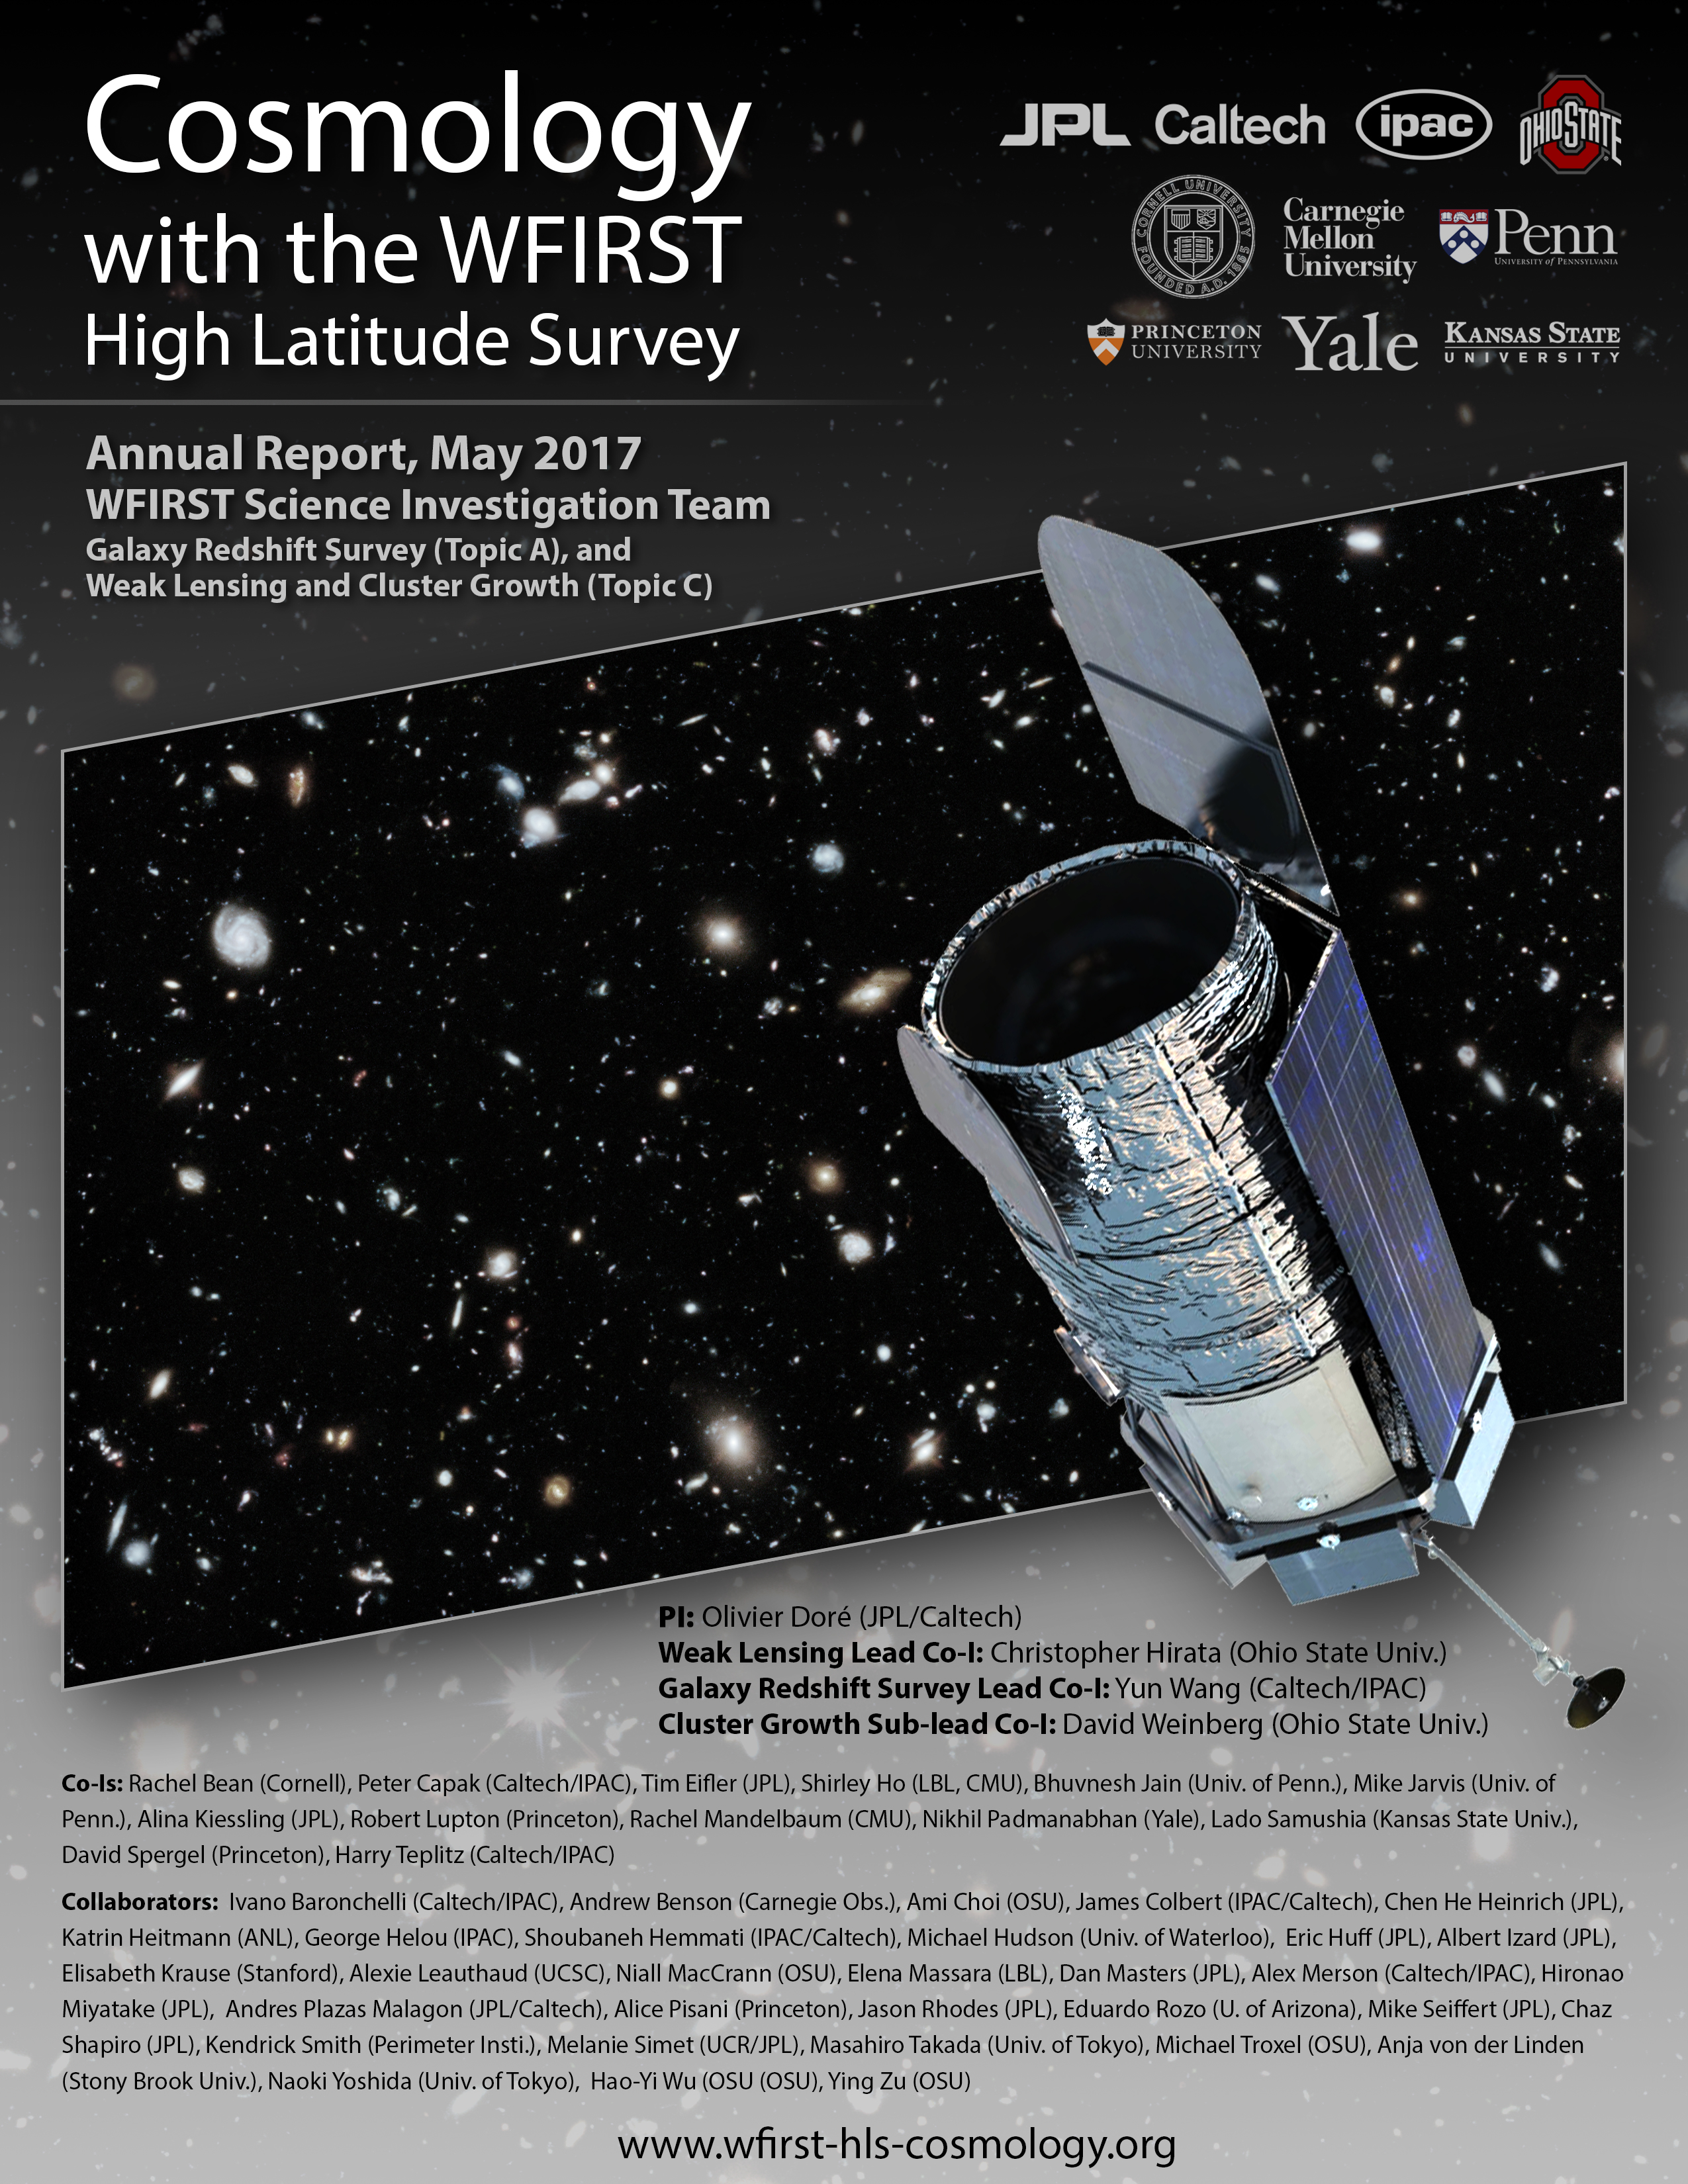
\includegraphics[width=1.35\textwidth,height=1.24\textheight]{Plots/WFIRSTProposalCover_AnnualReport2017.jpg}
% == With hyperref
%\vspace*{-2.cm}
%\hspace*{-1.cm}
%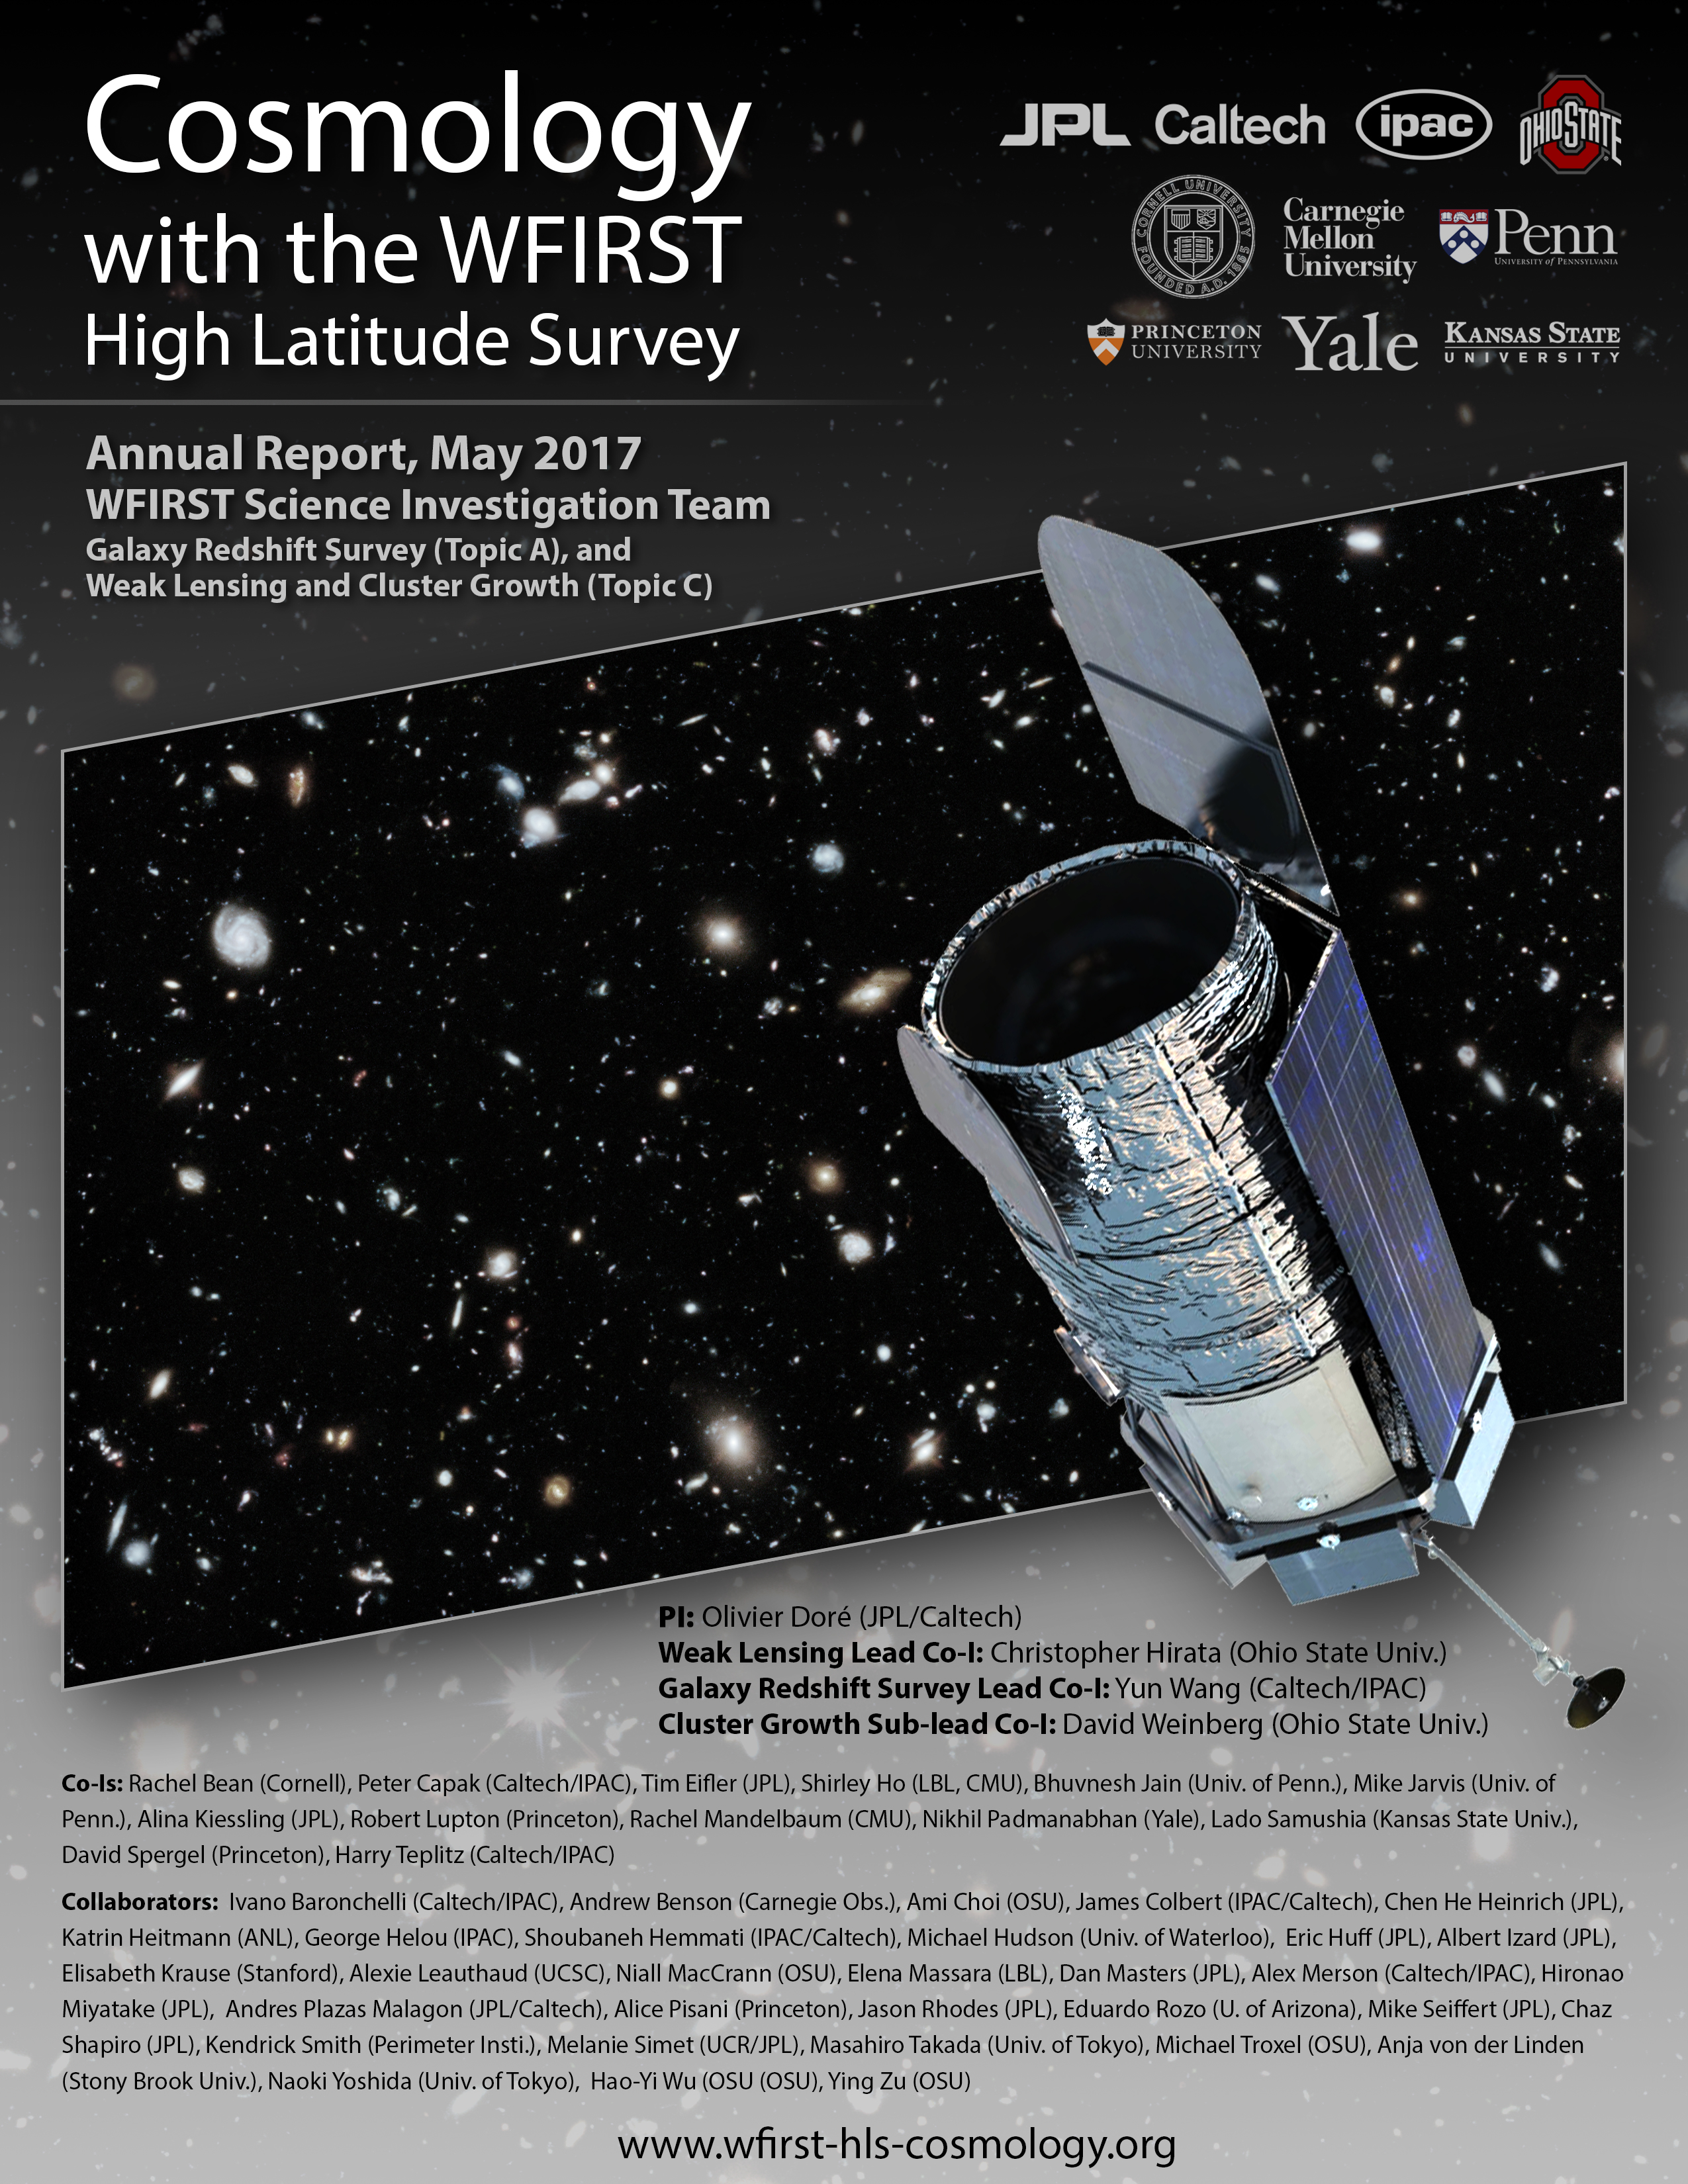
\includegraphics[width=1.35\textwidth,height=1.15\textheight]{Plots/WFIRSTProposalCover_AnnualReport2017.jpg}
%\thispagestyle{empty}
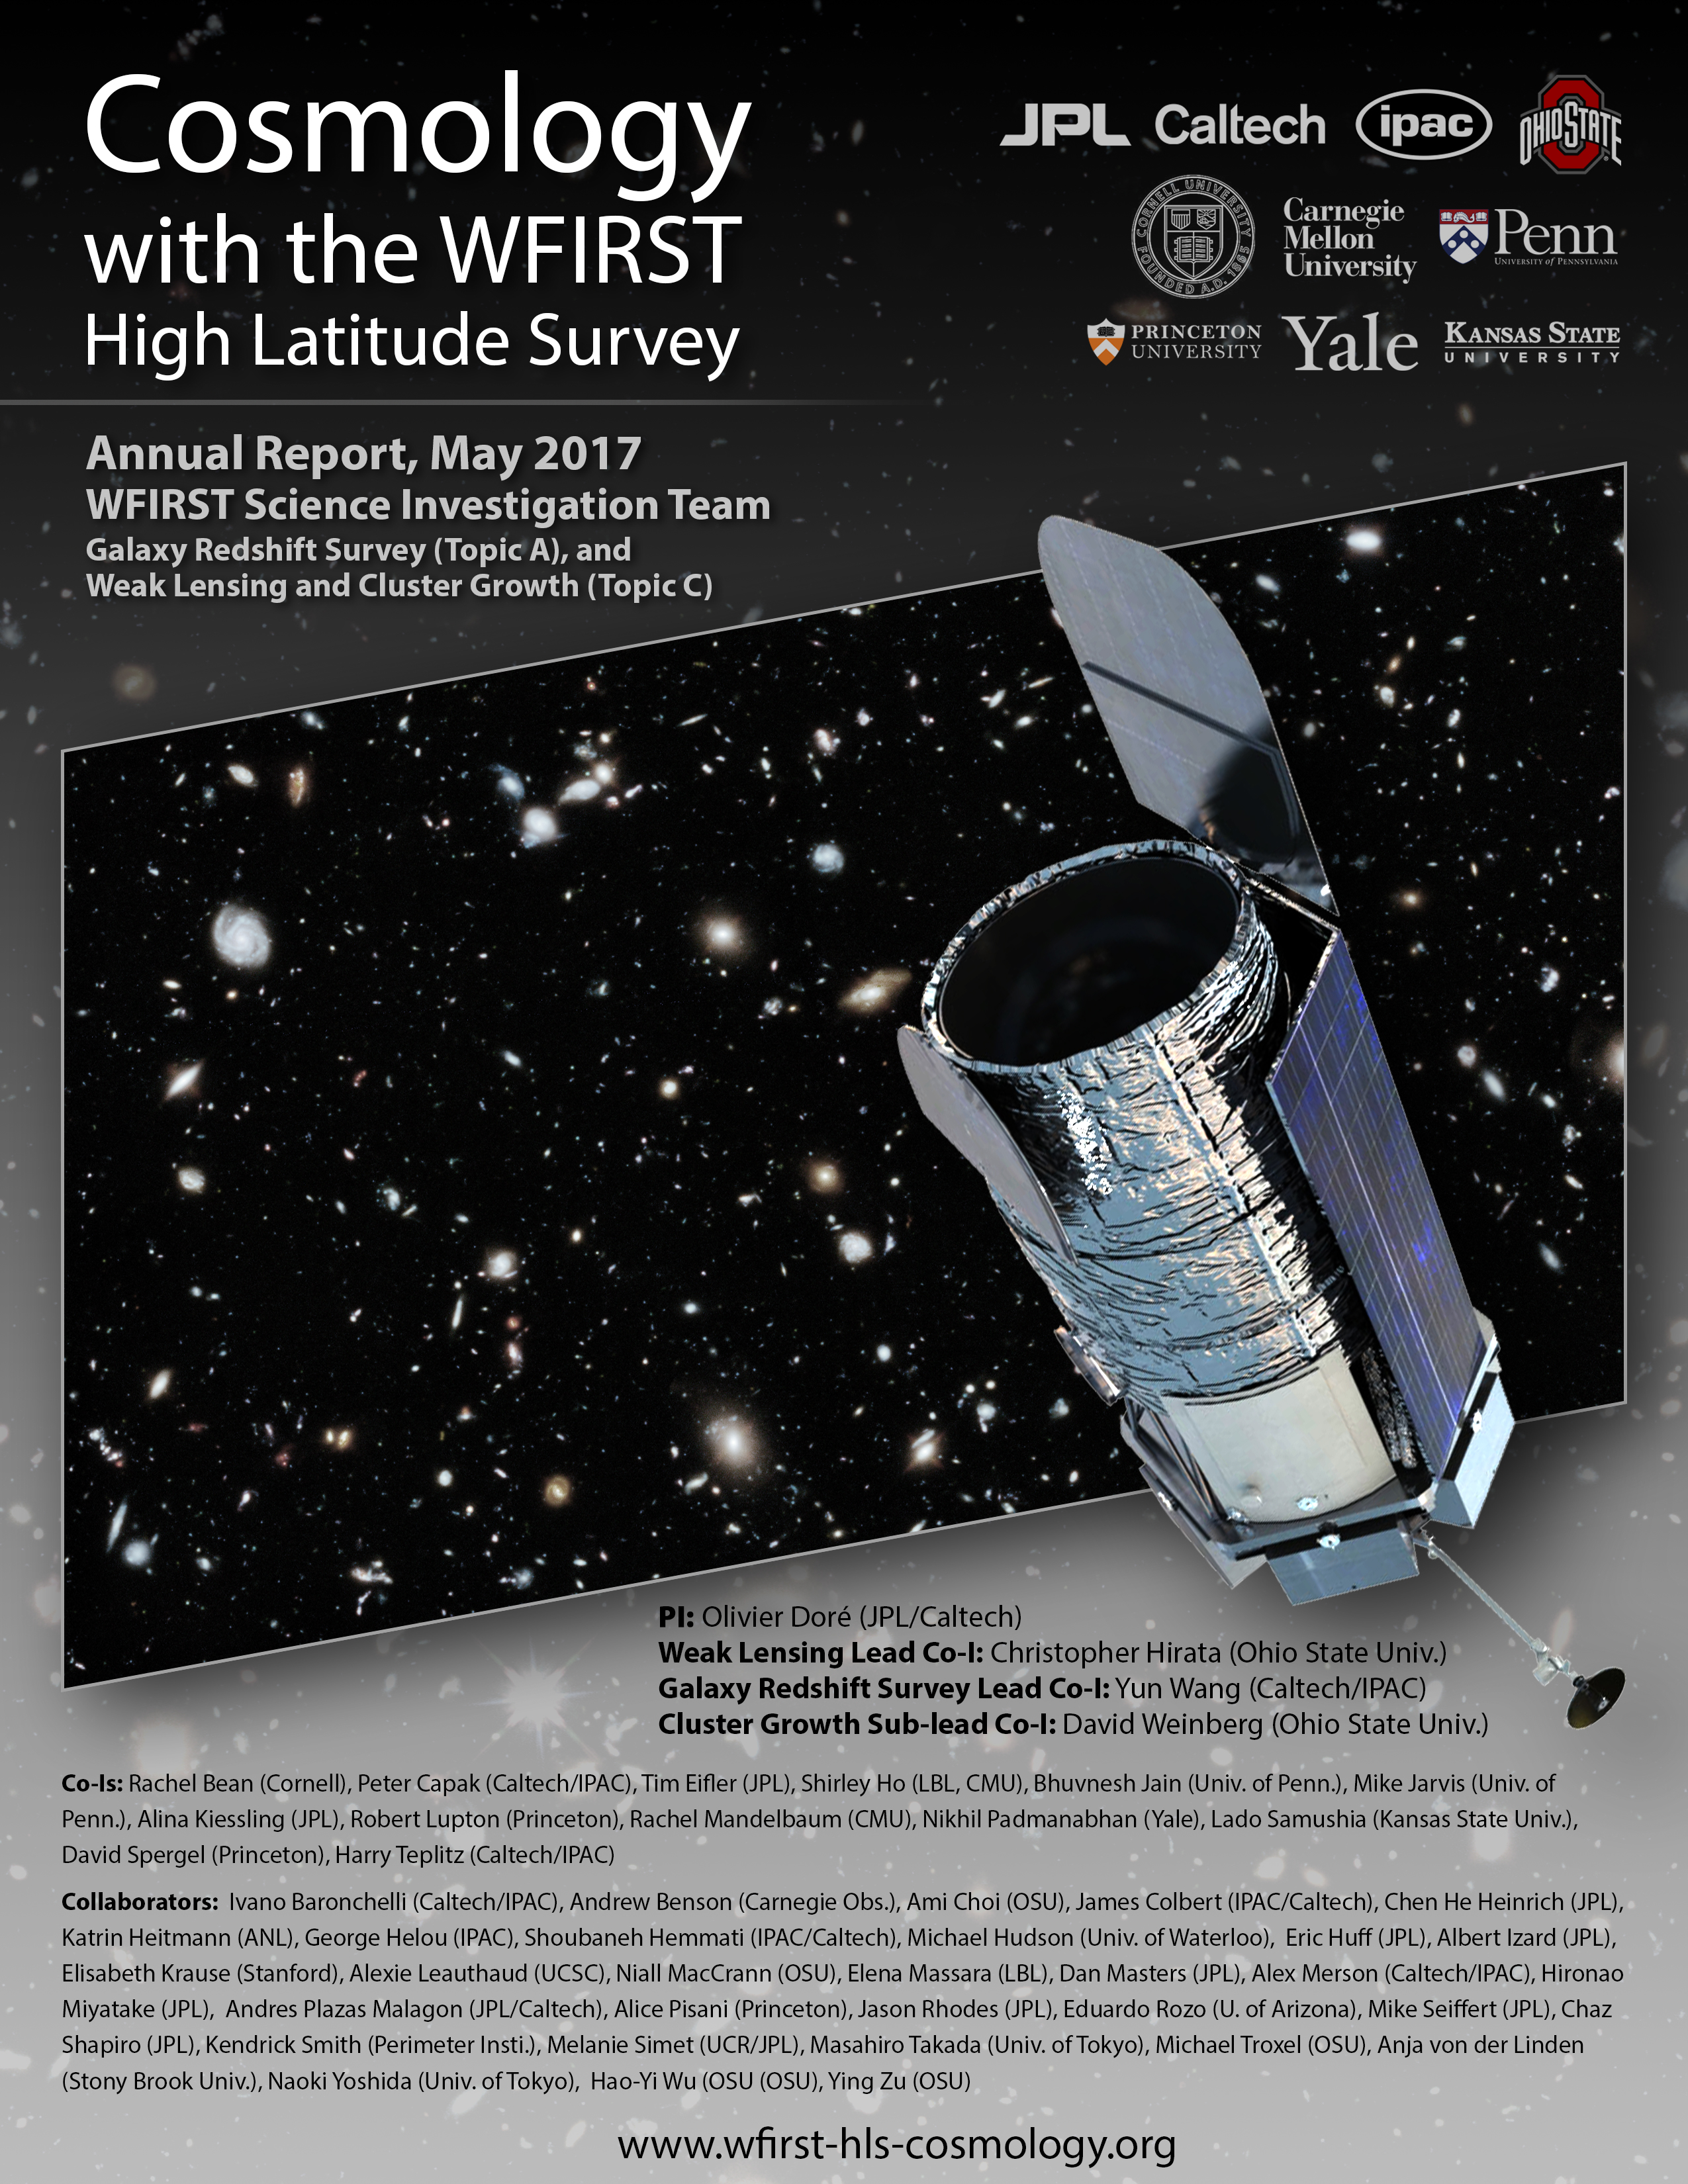
\includepdf[offset = 70 -80,height=11.3in]{Plots/WFIRSTProposalCover_AnnualReport2017.jpg}

\cleardoublepage


% Page header
\markboth{Cosmology with the WFIRST HLS Survey Science Investigation Team}{Annual Report 2017}

% Title
\title{Cosmology with the WFIRST High Latitude Survey \emph{Science Investigation Team}\\ Annual Report 2017}

\pagenumbering{roman}
\def\reff@jnl#1{{\rm#1\/}}

\newcommand{\jcap}{{\rm JCAP}}
\def\aj{\reff@jnl{AJ}}                  % Astronomical Journal
\def\araa{\reff@jnl{ARA\&A}}            % Annual Review of Astron and Astrophys
\def\apj{\reff@jnl{ApJ}}                        % Astrophysical Journal
\def\apjl{\reff@jnl{ApJ}}               % Astrophysical Journal, Letters
\def\apjs{\reff@jnl{ApJS}}              % Astrophysical Journal, Supplement
\def\apss{\reff@jnl{Ap\&SS}}            % Astrophysics and Space Science
\def\aap{\reff@jnl{A\&A}}               % Astronomy and Astrophysics
\def\aapr{\reff@jnl{A\&A~Rev.}}         % Astronomy and Astrophysics Reviews
\def\aaps{\reff@jnl{A\&AS}}             % Astronomy and Astrophysics, Supplement
\def\baas{\reff@jnl{BAAS}}              % Bulletin of the AAS
\def\jrasc{\reff@jnl{JRASC}}            % Journal of the RAS of Canada
\def\memras{\reff@jnl{MmRAS}}           % Memoirs of the RAS
\def\mnras{\reff@jnl{MNRAS}}            % Monthly Notices of the RAS
\def\physrep{\reff@jnl{Phys.~Rep.}}
\def\pra{\reff@jnl{Phys.~Rev.~A}}         % Physical Review A: General Physics
\def\prb{\reff@jnl{Phys.~Rev.~B}}         % Physical Review B: Solid State
\def\prc{\reff@jnl{Phys.~Rev.~C}}         % Physical Review C
\def\prd{\reff@jnl{Phys.~Rev.~D}}         % Physical Review D
\def\prl{\reff@jnl{Phys.~Rev.~Lett}}      % Physical Review Letters
\def\pasp{\reff@jnl{PASP}}              % Publications of the ASP
\def\pasj{\reff@jnl{PASJ}}              % Publications of the ASJ
\def\skytel{\reff@jnl{S\&T}}            % Sky and Telescope
\def\solphys{\reff@jnl{Solar~Phys.}}    % Solar Physics
\def\sovast{\reff@jnl{Soviet~Ast.}}     % Soviet Astronomy
\def\ssr{\reff@jnl{Space~Sci.~Rev.}}     % Space Science Reviews
\def\nat{\reff@jnl{Nature}}             % Nature

 %Define collection of Journal abbreviations.

%\begin{abstract}
%Abstract text
%\end{abstract}

\maketitle

\tableofcontents
\thispagestyle{empty}

\newpage
\pagenumbering{arabic}

%=================================================
\section{Executive Summary \Oli{Olivier, 2 pages}}
%=================================================
\label{sec:executive_summary}
%
% ** SECTION 1 **
%

\begin{summary}

Cosmic acceleration is the most surprising cosmological discovery in
many decades.  Even the least exotic explanation of this phenomenon
requires an energetically dominant component of the universe with
properties never previously seen in nature, pervading otherwise
empty space, with an energy density that is many orders of magnitude
lower than naive expectations. Testing and distinguishing among possible  explanations requires cosmological
measurements of extremely high precision that probe the full history of
cosmic expansion and structure growth.
This program is one of the defining objectives of the Wide-Field
Infrared Survey Telescope (WFIRST), as set forth in the {\it New Worlds, New Horizons}
report (NWNH) \cite{NWNH2010}.  The WFIRST mission, as described in the Science
Definition Team (SDT) reports \citep[hereafter SDT13 and SDT15 respectively]{Spergel2013, Spergel2015}, has the ability to improve these
measurements by $1-2$ orders of magnitude compared to the current
state of the art, while simultaneously extending their redshift grasp,
greatly improving control of systematic effects, and taking a unified
approach to multiple probes that provide complementary physical information
and cross-checks of cosmological results.

We described in this document the activities of the Science Investigation Team (SIT) \emph{Cosmology with the High Latitude Survey}.
This team was selected by NASA in December 2015 in order to address
the stringent challenges of the WFIRST dark energy (DE) program through the
Project's formulation phase.  This SIT has elected to address Galaxy Redshift Survey (GRS), Weak Lensing (WL) and Cluster Growth (CL) of the WFIRST Science Investigation Team (SIT) NASA Research Announcement (NRA) with a unified team, because the two investigations are tightly linked at both
the technical level and the theoretical modeling level. Our team thus fully embrace
the fact that the imaging and spectroscopic elements of the High Latitude Survey
(HLS) will be realized as an integrated observing program, and they jointly
impose requirements on instrument and telescope performance, operations, and
data transfer. We also naturally acknowledge that the methods for simulating and interpreting weak lensing and
galaxy clustering observations largely overlap. Many members of our team
have expertise in both areas.
%The WFIRST supernova cosmology program (investigation B) is more
%distinct in its methods and requirements, so it is feasible to
%integrate the supernova and HLS investigations at the level of the
%Formulation Science Working Group (FSWG).

In our proposal, we structured our planning around the series of deliverables
described in \S \ref{sec:deliverables}. We will present in this detailed report our progress on
these deliverables and illustrate that we either reached or exceeded our proposed
expected milestones.

Because development of requirements is at the core of our proposed
investigation, we present some broad aspects of our strategy in \S
\ref{sec:reqt_philosophy} before giving a summary of the High Latitude Imaging
Survey (HLIS) and of the HLS Spectroscopic Survey (HLSS) as we formulated them
to support the WFIRST Project Office in \S \ref{sec:wl_gal-clusters} and \S
\ref{sec:gc}. We present our revised cosmological forecasts and associated trade studies in
\S \ref{sec:forecast}. We also address questions of survey operations and
optimization in \S \ref{sec:operation}, our plans for broad community engagement
in \S \ref{sec:engagement} and discuss in \S \ref{sec:other_contributions} the
other ways in which our SIT supported the WFIRST mission.
%We conclude with a quick outline of the expected milestones for the coming year in \S
%\ref{sec:workplan}.
\end{summary}

%\addcontentsline{toc}{section}{References}
%We highlighted in bold the team members in the following bibliography.


%The team PI, Olivier Dor\'e, is a cosmologist with broad expertise in
%cosmic microwave background and large scale structure (LSS) studies. He brings
%extensive experience with complex data analysis (e.g., the Wilkinson
%Microwave Anisotropy Probe (WMAP), Planck) and mission design (e.g.,
%Joint Dark Energy Mission (JDEM) Destiny and the
%SMall EXplorer (SMEX) concept SPHEREx currently
%under Phase A study, for which he is the Project Scientist). Yun Wang
%and Chris Hirata will serve as Lead Co-Investigators for topics A and C,
%respectively and David Weinberg will serve as Lead for sub-topic
%``Cluster growth'' within topic C.  Many members of our team have been involved with the
%design and requirements of a dark energy space mission for a decade or
%more, including the Co-Chair (Spergel) and four additional members
%(Hirata, Hudson, Wang, Weinberg) of the 2013-2015 WFIRST-AFTA SDTs.  Our team
%includes authors of the two most comprehensive reviews of observational
%methods for probing dark energy \cite{Wang2010, Weinberg2013} and the
%Chair and Vice-Chair (Spergel, Weinberg) of the Astro2010 Science
%Frontier Panel on Cosmology and Fundamental Physics, whose report played
%a central role in the NWNH recommendation of WFIRST as the highest
%priority large space-based program.  Our team of Co-Is includes world
%leading experts on image processing and weak lensing (Eifler, Jain,
%Jarvis, Kiessling, Lupton, Hirata, Mandelbaum), on design and
%analysis of galaxy redshift surveys (Ho, Padmanabhan, Samushia, Wang, Weinberg),
%on space-based slitless spectroscopy analogous to that planned for WFIRST
%(Teplitz), on photometric calibration (Padmanabhan), on photometric
%redshifts (Capak) from large imaging surveys, and on cosmological forecasting
%%and parameter estimation from combinations of cosmic microwave
%background (CMB), WL, and LSS data (Bean, Dor\'e, Eifler,
%Hirata, Ho, Jain, Mandelbaum, Samushia, Spergel, Wang, Weinberg).

%Through this team of Co-Is, we have close connections to most of the
%major current or planned cosmological experiments that will provide
% This team of Co-Is brings close connections to most of the
%major current or planned cosmological experiments that will provide
%the context for the WFIRST dark energy program. This includes the WMAP and Planck CMB missions,
%the Sloan Digital Sky Survey (SDSS), the Baryon Oscillation Spectroscopic Survey (BOSS), the Dark Energy Survey (DES),
%the Subaru Hyper Suprime-Cam (HSC) and Prime Focus Spectrograph (PFS)
%projects, the Dark Energy Spectroscopic Instrument (DESI), the
%Euclid mission and the Large Synoptic Survey Telescope (LSST) Dark
%Energy Science Collaboration (DESC). Our team of U.S. and
%international collaborators brings extensive expertise in detector
%characterization, cosmological simulations, detailed simulations of
%observational data sets, and the theoretical modeling and cosmological
%interpretation of weak lensing and galaxy clustering data.
%Notably, members of our team are responsible for nearly all of the tables
%and figures in \S\S\ 2.2.3-2.2.5 of the SDT15 report, describing the
%HLS dark energy program.  We therefore have an unparalleled understanding
%of the current design of WFIRST-AFTA and of the
%challenges ahead in achieving its science goals.



%=====================================================
\section{Proposed Deliverables \Oli{Olivier, 4 pages}}
%=====================================================
\label{sec:deliverables}
%In \S\S \ref{sec:reqt_philosophy},\ref{sec:wl_gal-clusters},\ref{sec:gc}, we
%describe our work plan and explain how we will iteratively flow down science objectives to the
%measurements to be conducted, develop observational strategies,
%simulate synthetic astronomical `truth' data and the observational
%data output (including calibration), develop a methodology for
%validating dark energy constraints, and define scientific performance
%requirements and a complete plan for the science investigation.
%Our work plan maps the six SIT tasks into the deliverables below. For each deliverable, we identify in parentheses the required tasks (numbered \textit{T 1-6} as in \S 3.1 of the WFIRST SIT call). We will also associate explicitly the sections of our proposal to the deliverables.

\begin{summary}
In our proposal, we structured our planning around a series of deliverables
numbered D1-12. We will use throughout this report the same nomenclature and
report on our progress on each of these deliverables when compared to the
proposed calendar visible in Figure~\ref{tab:milestones_mgt}. We will
illustrate that we compare favorably on all deliverables. We give in this section a quick summary but will give more details in the relevant sections. We will also
explicitly reference  the deliverables (D1-12) in the relevant section titles of our report. In the text below, the definition of each deliverables is quoted directly from our proposal and we summarize the progress briefly in italic.
\end{summary}

% We will present in this detailed report our progress on these deliverables and
% illustrate that we either reached or exceeded our proposed expected milestones.

%Our work plan maps the six SIT tasks,  identified in parentheses  (numbered \textit{T 1-6} as in \S 3.1 of the WFIRST SIT call), to the deliverables below.
%For each deliverable, we identify in parentheses the required tasks.

%a given deliverable it encompasses.
%  For each
% deliverable,

%  In
% order to map our work plan into the six SIT tasks and our list of
% deliverables, we explicitly associate the subsequent sections with
% these deliverables.


%\subs{Program Milestones.} In Fig.~\ref{tab:milestones_mgt} we outline milestones for
%our effort in conjunction with the project timeline.\setlength\intextsep{-2pt}
\begin{figure}
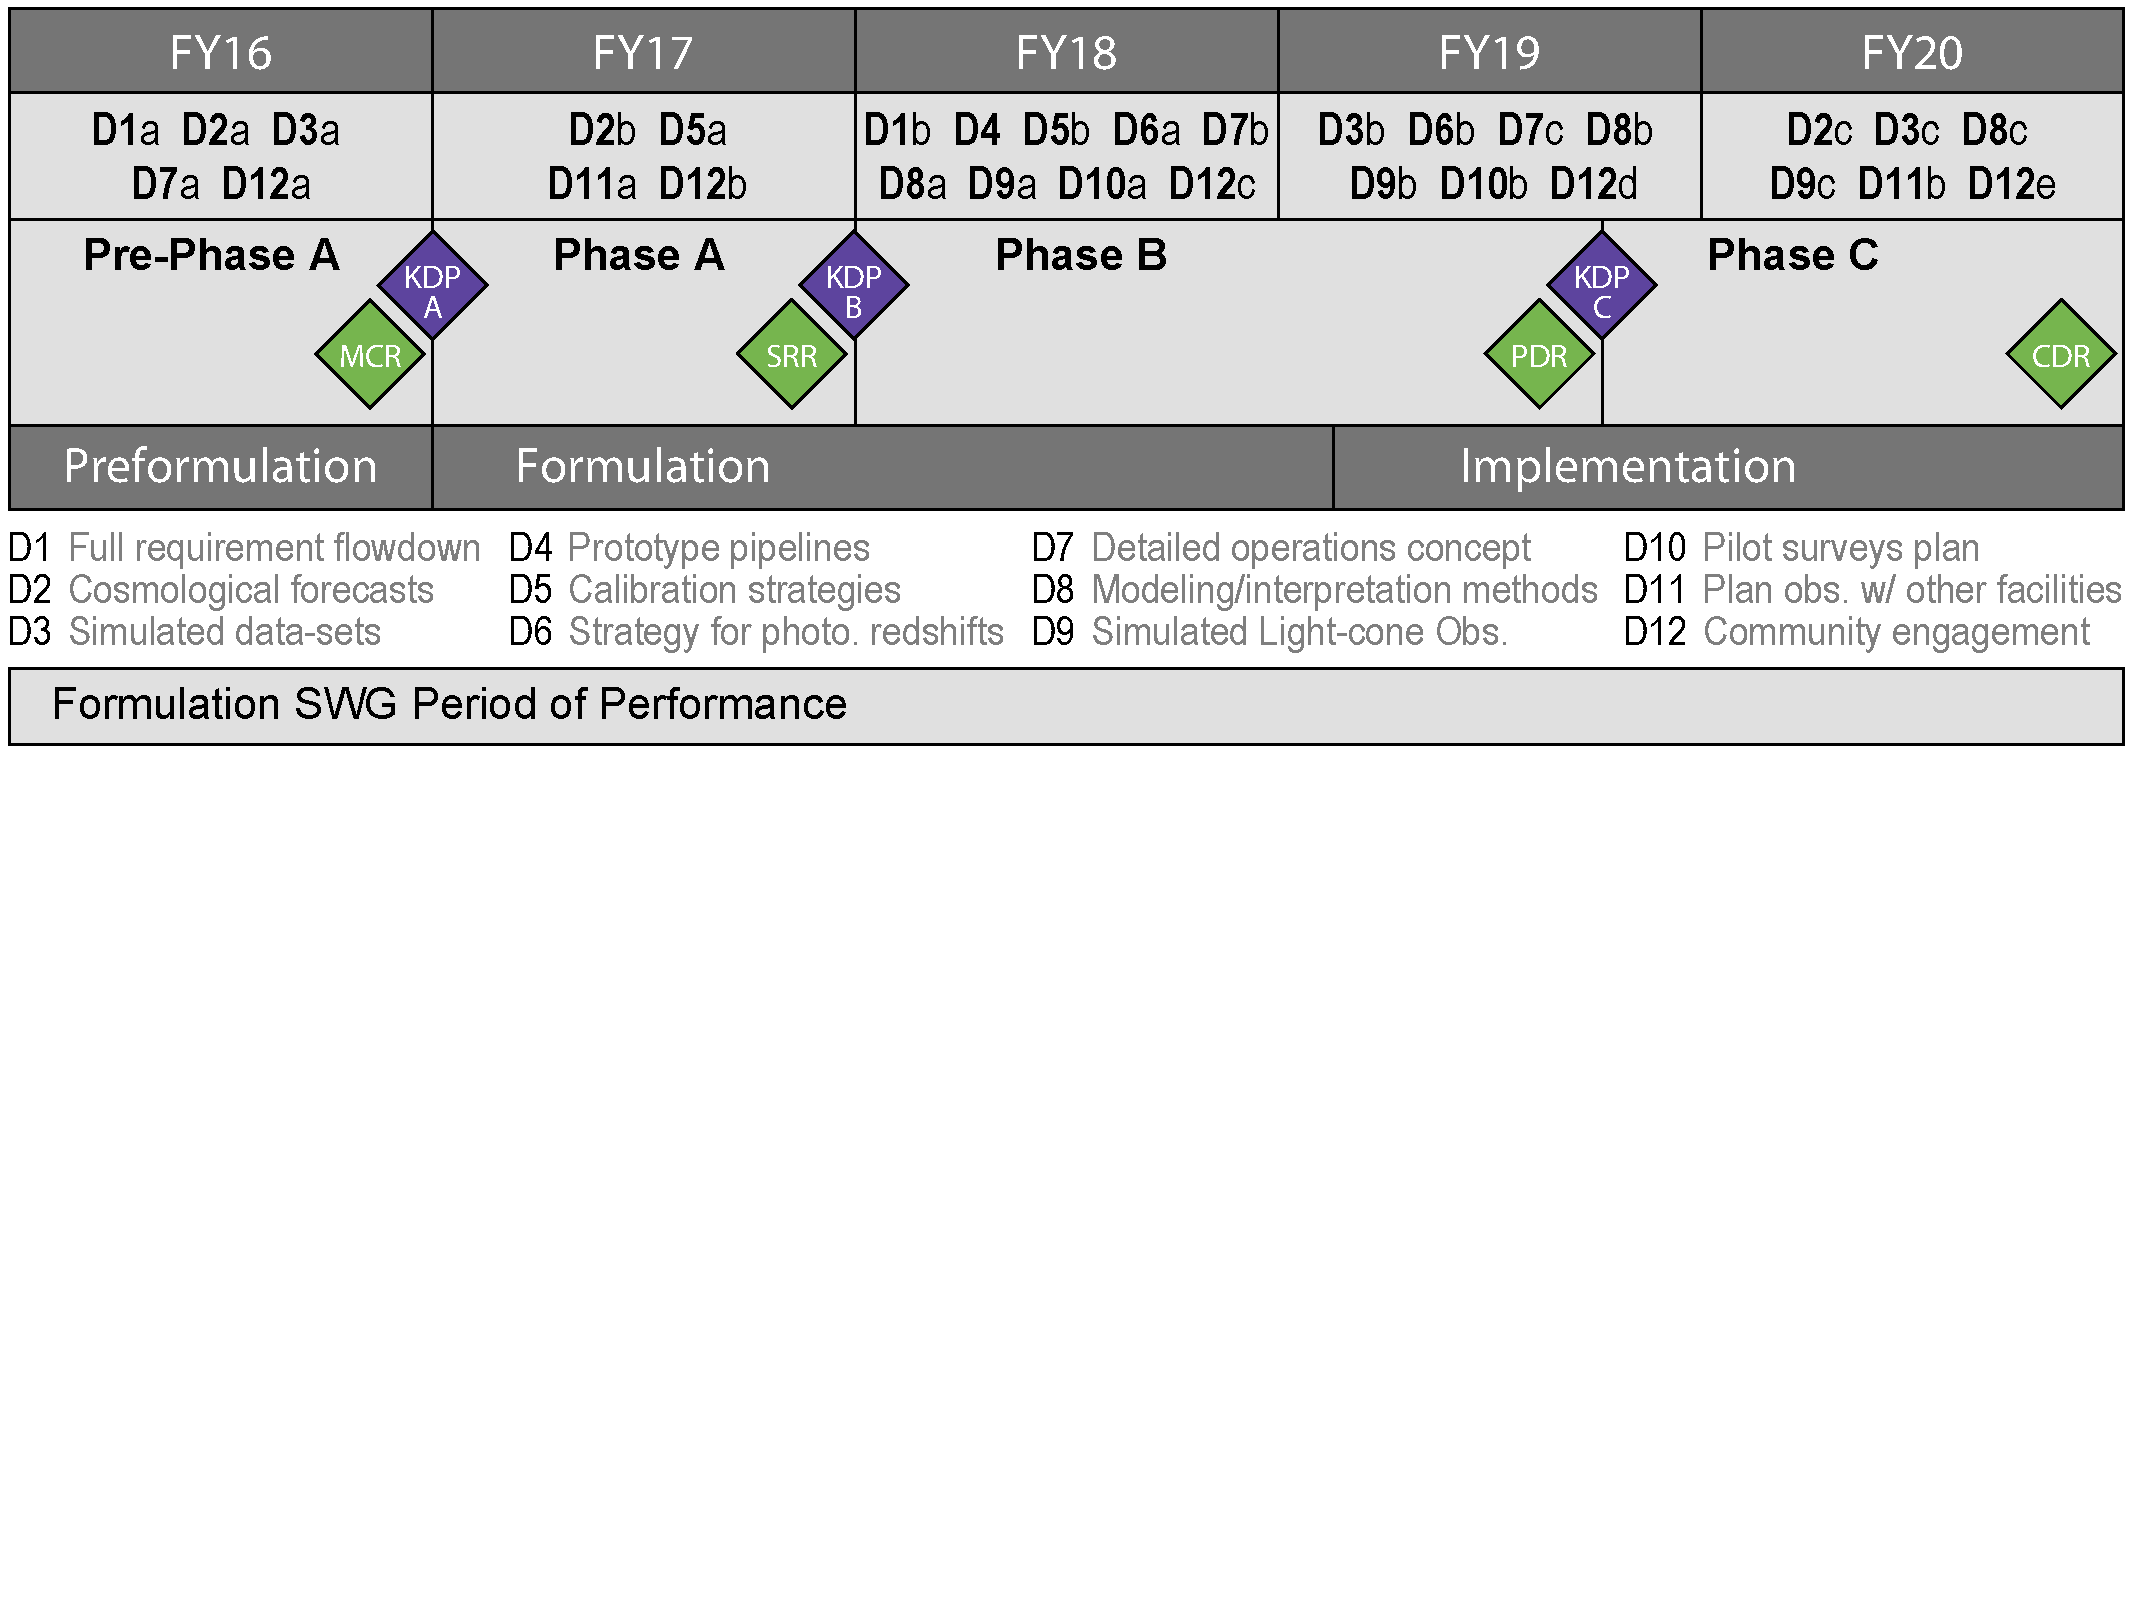
\includegraphics[width=0.99\textwidth]{Plots/wfirst_milestones_v2.pdf}
\caption{Our proposed deliverable schedule in concordance with the WFIRST
project timeline as displayed in the WFIRST SIT call \S 3.2. Deliverables that
are made in multiple stages are labeled (a, b and c) and appear in multiple
years. This figure is taken from our original proposal and the schedule has in
fact shifted since our investigation started on January 2016, thus well into
FY16.} \label{tab:milestones_mgt}
\end{figure}

\paragraph*{(D1) Full requirements flow-down} from the high-level science goals
of the HLS galaxy clustering and weak lensing survey to detailed performance of
the telescope, wide field instrument, software, operations, and data transfer.
\emph{Throughout the year, we delivered three versions of the level 2 science
requirements for both the HLSS (\S \ref{sec:gc}) and the HLIS (\S
\ref{sec:wl_gal-clusters})}.

\paragraph*{(D2) Forecasts of the cosmological performance of the HLS Imaging
and Spectroscopy data sets,} including expected constraints on dark energy,
modified gravity, neutrino masses, and inflation, from analyses that include the
measurement of the location of the Baryon Acoustic Oscillations (BAO),
Redshift-Space Distortions (RSD), galaxy power spectrum and higher order
statistics, cosmic shear, galaxy-galaxy lensing, and cluster demographics. These
forecasts incorporate realistic assessments of observational systematics and
theoretical modeling systematics, and they examine the expected constraints from
different probes individually, in concert with each other, and in concert with
expected constraints from the WFIRST supernova program, CMB experiments, and
other cosmological surveys such as DESI, LSST, and Euclid. We use our
forecasting tools to investigate trades, e.g., the impact of survey or
instrument design choices (area, depth, pixel size, spectral resolution, etc.)
on cosmological performance. \emph{We developed a unique software package (\CoLi) that
enables us to jointly forecast all the WFIRST cosmological probes, including
their covariance (\S \ref{sec:forecast}). We used this framework to conduct trade studies \S\ref{sec:forecast}. We released to the community the
associated WFIRST chains (\S \ref{sec:other_contributions})}.

\paragraph*{(D3) Simulated imaging and spectroscopic data sets} for testing pipeline
performance and evaluating systematic biases --- e.g., from confusion,
noise, and incompleteness in images and spectra, or errors in Point
Spread Function (PSF) determination or shape measurement.
These data sets will be created with varying levels of complexity
in the source catalogs and instrumental effects, to allow isolation
of individual contributions to statistical and systematic uncertainties.
Some of these artificial data sets will be made publicly available,
and some will take the form of data challenges, where the underlying
parameters are initially known only to the creators of the data set,
in the spirit of the Shear Testing Program (STEP) and Gravitational
Lensing Accuracy Test (GREAT) weak lensing data
challenges \cite{Heymans2006, Massey2007, Bridle2010, Kitching2012, Mandelbaum2015}. \emph{We implemented a WFIRST dedicated module in the state-of-the-art simulation image simulation pipeline GalSim and will release it to the community (\S \ref{sec:hlis_image_sim}). We will contributed mock observations to the SOC based image simulation effort for the HLSS}.

\paragraph*{(D4) Proto-type imaging and spectroscopic pipelines}, including weak lensing shape measurement and galaxy redshift measurement, tested against the
above artificial data sets. These proto-type pipelines will provide
building blocks for development of full pipelines during the implementation
phase, and they will allow us to sharpen definitions of software
requirements and to identify challenges to and strategies for meeting
these requirements. \emph{We started to develop dedicated quick tools that will allow us to built and evaluate a GRS pipeline (\S \ref{sec:grs_algo})}.

\paragraph*{(D5) Calibration strategies} for photometry, shape measurement, spectroscopy, and redshift completeness. Evaluation of the expected performance of these strategies against the science requirements. The requirement on knowledge of the dark current and the calibration approaches are fully defined, based on analysis done during the dark filter trade (October 2016 -- February 2017). \emph{We contributed extensively to the WFIRST WFI Calibration Plan. This includes extensive quantitative analysis of proposed calibration techniques (\S \ref{sec:calibration_plan})}.

\paragraph*{(D6) A strategy for the determination and calibration of photometric redshifts} using WFIRST data and anticipated external data (e.g., LSST optical
photometry), and defining ground-based data that are needed to
implement this strategy (e.g., spectroscopic training sets, large
redshift surveys for calibration via cross-correlation).
Evaluation of the impact of remaining photometric redshift uncertainties
on statistical and systematic errors in weak lensing and clustering analyses.
Definition of requirements for WFIRST photometric redshifts informed
by this strategy and evaluation. \emph{We made substantial progress by co-leading a large dedicated spectroscopic observation program (C3R2), generating mock WFIRST and LSST observations based on HST CANDELS data (\S \ref{sec:wl_photoz}), by devising calibration strategies based on Self-Organized Maps (\S \ref{sec:wl_photoz}), and by studying the importance of the Integral Field Channel (IFC) to calibrate photometric redshifts (\S \ref{sec:forecast})}.

\paragraph*{(D7) A detailed operations concept for the HLS Imaging and Spectroscopy
program,} extending the work presented in SDT13 and SDT15. \emph{In collaboration with the relevant WFIRST WG, which we are co-leading, we delivered to the project multiple detailed updates to the operation concept (\S \ref{sec:operation}) and propagated it into image simulations (\S \ref{sec:hlis_image_sim}) and forecasts (\S \ref{sec:forecast})}.

\paragraph*{(D8) Development of methods for modeling and interpreting the cosmological
measurements anticipated from WFIRST}. Determination of the effects of non-linear gravitational clustering, realistically complex relations between the
galaxy and dark matter distributions, and the influence of the baryon
component on matter clustering. The study of techniques to
remove systematic biases, e.g., by marginalization over nuisance
parameters. Utilization of cosmic shear, galaxy-galaxy lensing, cluster mass functions and cluster weak lensing, BAO, RSD, the galaxy
power spectrum, and higher order statistics for galaxy clustering, weak
lensing, and various combinations. Identification of areas where
further improvements of theoretical modeling would significantly
enhance the cosmological return from WFIRST. \emph{We have not started to work on this deliverable yet besides generating realistics mock observations (\S \ref{sec:light-cone})}.

\paragraph*{(D9) Simulated light-cone observations} based on cosmological simulations for guiding this methodology development and testing its performance.
Most of these data sets will be at the level of galaxy redshift and shape
catalogs rather than the pixel-level imaging and spectroscopy simulations
described above.  They will incorporate varying degrees of complexity
regarding galaxy bias, redshift evolution, survey geometry, and
observational systematics such as incompleteness, shape measurement errors,
and photometric redshift biases.  Many of these artificial data sets
will be made publicly available, and some will take the form of data
challenges, where the underlying parameters are initially known only
to the creators of the data set. \emph{We started assembling multiple light-cone observations dedicated to GRS, but also WL+GRS (\S \ref{sec:light-cone}) and expect to release the catalogs in the coming months. We published one dedicated paper (\S \ref{sec:other_contributions})}.

\paragraph*{(D10) Pilot survey proposals with associated figures of merits,} to
be executed during the first months of WFIRST operations. These would become
part of the final dark energy data set but also pin down remaining astrophysical
or instrument performance uncertainties at the level needed to optimize the HLS.
We will develop the figures of merit required to quickly assess the data-quality
and make operational decisions regarding the cosmological surveys. \emph{This
activity has not started yet beyond discussions of the deep fields, in
conjunctions with the other SITs and other major observational efforts during
our community workshop (\S \ref{sec:engagement})}.

\paragraph*{(D11) A prioritized program of observations from other facilities,}
ground and space-based, needed to calibrate or finalize strategy decisions on
the WFIRST dark energy program. \emph{Members of our SIT are leading an
ambitious spectroscopic observations campaign (C3R2) aiming at calibrating photometric redshifts
for WFIRST and other surveys. Members of our team are leading a major
observational program on Spitzer (the Spitzer Legacy Program (SLS)) to prepare for WFIRST and others. We expect this type of activity to be the focus of our second community workshop (\S \ref{sec:engagement}).}

\paragraph*{(D12) Broad engagement with the cosmological community,} through
workshops, talks, publications, and public release of codes and artificial data
sets, with the goals of (a) building awareness of and broad support for the
WFIRST dark energy program and (b) inspiring the community to develop methods
and carry out investigations that will maximize the cosmological return from
WFIRST. \emph{We organized in September 2016 our first community workshop in
Pasadena. It was dedicated to enabling the scientific synergies between WFIRST HLS and
LSST DESC (\S \ref{sec:engagement}). Our second community workshop dedicated to
synergies between WFIRST HLS and other surveys is scheduled for the fall 2017. We also
released new software packages, enhanced data products and forecasts (\S
\ref{sec:other_contributions}). We published 11 papers inspired by WFIRST (\S
\ref{sec:other_contributions})}.


%\vspace{-0.15in}
%%================================================
%\section{Requirement Philosophy (D1)}
%================================================
%\label{sec:reqt_philosophy}
%%
% ** SECTION 4 **
%

\begin{summary}
The WFIRST science requirements process connect HLS
hardware and software requirements to statistical and systematic error budgets
and in turn to  cosmological constraints. While nominally a ``flow-down",  in
practice it is an iterative process as we optimize the science return within
engineering  constraints. We use different tools for each part of this process.
\end{summary}

At the highest level, we  use the \CoLi\ forecasting package to relate cosmological
constraints to data set parameters (sky coverage, galaxy density) and
parameterized descriptions of the systematic error budget. \CoLi\ is a
multi-probe analysis and forecasting pipeline that is unique in its integrated
ansatz of jointly modeling LSS probes and their correlated statistical and
systematic errors. \CoLi\ incorporates a full exploration of parameter space in
place of the Fisher formalism, and it incorporates a range of astrophysical
(e.g., intrinsic alignments, nonlinear galaxy bias, baryonic effects) and
observational (e.g., shear calibration, photo-$z$ uncertainties) systematics. It
is actively maintained and updated as part of our support of the FSWG.

%Planned work includes adding new science extensions (spatial
%curvature and neutrino masses), WFIRST-specific systematic uncertainties, and the addition of higher order statistics to exploit the potential science return from the high number density of galaxies

% Our team members have  applied it to SDSS WL data \cite{Huff2014},
%LSST forecasts \cite{Krause2015}, and DES data
%\cite{Becker2015, DES2015}. \CoLi\ incorporates a full exploration of
%parameter space in place of the Fisher formalism, and it incorporates a range
%of astrophysical (e.g., intrinsic alignments, nonlinear galaxy bias, baryonic
%effects) and observational (e.g., shear calibration, photo-$z$ uncertainties)
%systematics.
%Eifler and Krause will actively maintain and
%update \CoLi\ as part of our support of the FSWG.  Planned work includes adding new science extensions (spatial
%curvature and neutrino masses), WFIRST-specific systematic uncertainties, and the addition of higher order statistics to exploit the potential science return from the high number density of galaxies
%in the imaging and spectroscopic surveys.

%CosmoLike represents a major leap beyond the previous generation of forecasting tools (e.g. those written for the SDT by Co-I Hirata), which will be used only as secondary checks.

WFIRST hardware capabilities (e.g., throughput, slew times) and observing
strategy/time allocation determine the HLS's statistical power, whereas the
ability to robustly constrain the instrument response model and astrophysical
nuisance parameters determine the systematic errors. Statistical errors
generally vary continuously as hardware parameters are changed, so the hardware
requirements will reflect a joint assessment of science performance and
engineering capabilities (including cost and risk). For the science assessment,
we built on our previous work on the Exposure Time Calculator (ETC) and
operations simulations codes (both written by Co-I Hirata).  Both sets of tools
are fully automated and can treat the WL and GRS surveys with a common set of
scripts. We built an interface from these tools to \CoLi\ so that
we can evaluate the science impacts of changes in WFIRST requirements (e.g., the
static wavefront error budget). Our team  work in close coordination with
project engineers to carry out a cost/benefit analysis of each such trade.

% Co-I Hirata has played this role extensively on the WFIRST SDTs and will be the lead
%for this task.

%
% Not sure that this paragraph is essential
%
% C.H. -- I think we need to discuss our approach to systematics here, as they are an important part of the error budget. I've tried to compress this as much as I can.
%
%Where practical, we will set the systematic error budget by requiring that their combination be smaller than the expected statistical errors. Two approaches are possible:
%(i) to require the systematic in the observable (e.g. shear power spectrum) to be smaller than the statistical errors; and (ii) to require errors on e.g. $w$ to be
%increased relative to statistical-only errors by some factor. Our preference is for (i) as it leads to simple and robust error budgeting: independent systematics can be
%quadrature-summed, the requirement does not change if new cosmological parameters are added (e.g. neutrinos) or if external data sets are added, and no internal
%consistency tests in the data are lost. In cases where such a tight systematic error budget becomes a cost or risk driver, we may in consultation with the Project
%formulate a requirement using criterion (ii). Due to the potential for complex interactions among different systematics, all such instances will be explicitly tracked in
%the forecasting machinery.
%
%Where practical, we will set the systematic error budget by requiring that their combination be smaller than the expected statistical errors. Our preferred approach is to
%set systematics requirements in the observable space (e.g., shear power spectrum) rather than in terms of marginalized errors on $w$, since this leads to robust
%error budgeting: independent systematics can be quadrature-summed, the requirement does not change if new cosmological parameters or external
%data sets are added, and no internal consistency tests are lost. We will back away from this approach only if such a tight systematics budget becomes a
%cost/risk driver. We will flow the systematics requirements down to the hardware (e.g., stability) and operations (e.g., survey
%cross-linkage) using quantitative forecasting tools, for example predicting the covariance matrix of the flat field uncertainties. Co-I Hirata will be the lead
%liaison with the Project team for these studies.
%
%Finally, we will develop the error budget validation methodology.  We will develop a list of systematic error control tests on the WL and GRS data and derive the requirements on the observing program.
%
%%and may require us to accept statistical power below the maximum theoretically achievable. We
%%%will quantitatively assess the constraining power of the validation tests as we optimize the survey design and hardware requirements.


%======================================================
\section{Weak Lensing and Cluster Growth Investigation}
%======================================================
\label{sec:wl_gal-clusters}
%
% *** SECTION 5 ***
%

As discussed in \S 2.2.3 of SDT15 (written by members of our team), the
HLS Imaging survey will (in its current design) measure the shapes of
nearly 400 million galaxies in 3 near-infrared (NIR) bands, plus fluxes in a 4th band
to improve photometric redshifts (photo-$z$).  With a data set two orders-of-magnitude
larger than the current state of the art \cite{2012MNRAS.427..146H,Becker2015},
the WFIRST weak lensing program will
measure the cosmic expansion history and the growth of structure with
exquisite statistical precision, demanding corresponding advances in the
control of WL systematics.  The cosmic shear power spectrum, which is the
basic WL observable, depends on both the distance-redshift relation $D(z)$
and the power spectrum of matter clustering $(\Omega_m h^2)^2 P_m(k,z)$.
The WL survey will also enable high-precision cosmological constraints
from galaxy-galaxy lensing (GGL) and from galaxy clusters, which can be
identified in either the HLS or external data sets and characterized with
the help of WFIRST WL.  The \CoLi\ forecasting tool can predict the constraints
from these methods individually and in combination with complementary
probes such as BAO, RSD, supernovae, and the CMB.
While all aspects of our investigation are interconnected, we
separate the discussion into more tightly connected loops: requirements,
image simulations, and algorithm development at level of pixels and shape measurement;
issues related to photometric calibration and photometric redshifts;
development of methods for cosmological analysis of WFIRST
data and testing them on simulated data; and finally methods for
systematic error testing and mitigation.

\subsection{Requirements (D1, D3, D4, D5)}
\label{sec:wl_requirements}
%================================================
\Auth{Chris, Rachel M, Mike}

The definition of WFIRST requirements will
%proceed through a phased approach with several
%stages of increasing detail and maturity,
start in pre-Phase A and continue through
CDR. In the early stages, we will focus on identifying the driving requirements for the
mission (e.g., those related to total throughput, wavefront error and wavefront stability,
and any calibration requirements that would require dedicated hardware or special operational modes).
Simple simulation tools will be used for this stage, where fast turnaround times and
conservative assumptions will be prioritized over the true end-to-end simulations that
will be required for the analysis. As the project matures, we will consider the more
complete list of requirements (e.g., specifications on data products)
and work with the WFIRST Science Centers (WSC) to build the fully
realistic simulations needed to test reduction and analysis pipelines.

Our existing tools (the ETC, operations simulations, and \CoLi)
allow us to forecast the statistical power of the WL survey for a specified
observing strategy and time allocation and to evaluate the impact of
hardware or strategy changes on cosmological constraints (see \S 6.2).
The challenge for the SIT is to define requirements that ensure control
of systematic uncertainties at the level of these statistical errors.
WL systematics fall into two broad categories, instrumental/algorithmic
effects tied directly to the measurements and astrophysical effects
tied to the cosmological interpretation of the measurements.  The former
affect engineering requirements, while the latter must be predicted
theoretically or constrained through observations.

Our basic strategy for defining instrumental/algorithmic requirements
is to create simulated HLS images with varying levels of realism, analyze
them with proto-type data reduction and WL pipelines, and compare the
resulting measurements to the simulation inputs. We will determine
the sensitivity of WL shear measurements to each effect,
and then flow down requirements from nuisance parameters in
\CoLi\ (e.g., spurious shear) to hardware requirements that can be compared to integrated
modeling results (e.g., wavefront stability).
Our simulation
framework will build on the public code {\tt GalSim} \cite{2015A&C....10..121R}, which already
includes a WFIRST-AFTA module and
to which Co-Is Jarvis and Mandelbaum are lead contributors.  Our proto-type pipelines will
build on codes for image analysis and shear measurements developed
over many years by Co-Is Hirata, Jarvis, Lupton, and Mandelbaum
and their collaborators for analysis of SDSS, DES, HSC, and LSST imaging
\cite{Lupton2001, 2003MNRAS.343..459H, 2005MNRAS.361.1287M,
2012MNRAS.420.1518M, 2011arXiv1111.6958H, Jarvis2015}.
WL algorithms are an active area of research,
and we will integrate promising new approaches as our investigation
progresses.  Our overall framework is analogous to, but more %tightly
focused than, the GREAT3 challenge led by Mandelbaum \cite{2014ApJS..212....5M},
including the use of different simulation branches where effects are turned on and off
(separately or together) to probe the %origins of any
biases %or unexpected behaviors
resulting from individual or combined effects.
%we will draw on lessons learned from this effort and its predecessors.

In the domain of instrument- and pipeline-related systematic errors,
each error must be evaluated according to the following criteria:
(i) What is the raw magnitude of the systematic error compared to statistical errors?
(ii) What is the approach to modeling and removing that systematic error? What cross-checks will be necessary to
validate that this has been done correctly? (iii) Are there
implications to the optimal observing strategy (e.g., dithering, repeat observations, dedicated calibration
observations)? (iv) Are there implications for the hardware requirements (e.g.,
stability, pre-flight characterization, or dedicated flight calibration hardware)?

As an example: optical aberrations induce PSF ellipticity that is 2 orders of magnitude
greater than WFIRST weak lensing requirements if uncorrected. It is not practical to
eliminate the effect in hardware by requiring the wavefront to be perfect at the few nm
level in a wide-field instrument, so a model of the PSF will have to be built.
Some contributions to the PSF (e.g., jitter and guiding errors) will need to be measured separately for each
exposure. Others vary on longer time scales (e.g., due to thermal changes in the optics)
and imply a trade-off between stability requirements
and the noise on a measurement of the relevant parameter from a set of $N$ exposures.
We will use these considerations to turn high-level requirements on knowledge of the PSF into
lower-level requirements on thermal stability and on the operations plan.

Detector systematics are special because their absolute amplitudes may be difficult for the vendor to control or even test.
We thus anticipate absolute
requirements only on the largest systematic effects such as inter-pixel capacitance (IPC) and persistence, which are
being addressed as part of the technology development program. There will be many subtler
effects arising in the detectors
(examples might include NIR-detector analogues of the brighter-fatter effect,
color-dependent charge diffusion, etc.); we will set requirements on the knowledge of these.
We will pay special attention to methods of measuring these effects on-orbit using a combination of
ground characterization, dedicated calibration modes, and the survey data itself,
and the interaction with survey operations and stability requirements (on e.g., focal plane temperature).
We will coordinate the best approach to these effects with the Project
and with collaborators Seiffert and Shapiro.  Shapiro leads the
Precision Projector Laboratory (PPL), a JPL facility designed to
emulate WFIRST weak lensing data using scenes focused onto WFIRST
NIR-detectors.  Systematics identified thusly will be studied and
mitigated in collaboration with the SIT.  Co-I Hirata advises the PPL on
image analysis software and interpretation of results \cite{Rowe:2011wj, Seshadri:2013xla}.

%We will treat astrophysical systematic errors differently because one cannot write
%a requirement on e.g., the behavior of a galaxy, so the requirements are instead on the
%algorithmic strategies for mitigating the systematic errors.
%A typical mitigation strategy for intrinsic alignments (IA) of galaxy shapes would involve
%jointly modeling the effects of IA on the
%tomographic two-point functions of the shear and the galaxies.
%As shown by, e.g.,
%\cite{2007NJPh....9..444B}, the need to marginalize over IA results in
%more stringent requirements on how well the photometric redshift error distributions are
%known.
%In some cases, the effects of astrophysical uncertainties are degenerate with measurement
%uncertainties; for instance the effect of baryonic physics on the lensing power spectrum
%is partially degenerate with photometric redshift errors \citep{2012JCAP...04..034H}.
%As we cannot place a requirement on baryonic physics, this can result in
%more stringent requirements for the effects we can control, such as photometric redshifts.

Cluster cosmology is generally considered to be less demanding in terms of hardware requirements than
cosmic shear, since the large galaxy over-densities and shear signals are not as easily masked by
subtle optical aberrations or detector behaviors. Nevertheless, it may place new requirements
on survey footprint/operations (to ensure overlap with other data sets); pipeline behavior in
crowded fields (e.g., \cite{2015MNRAS.449.1259S}); and ancillary data products and simulations to describe, e.g., changes in selection
effects and source redshift distributions in the presence of blending and magnification.
WL requirements lead Hirata will work closely with cluster lead Weinberg to ensure that these
requirements are captured in the flow-down.

% -- notes from DHW --
%
%\bi
%\item  Dark energy requirements for HLS Imaging and associated
% instrument requirements, at level of image sampling,
% PSF stability, software performance, etc.
%\item  Simulations at level of frames, focal plane.  Data challenges.
%\item  Proto-type pipelines that either meet requirements or inform
% what is needed to meet them.  Assessment of photometry errors,
% shape measurement errors.
%\ei
%
%DW comments on this subsection: Idea of proto-type pipelines is that
%they are capable of analyzing the same data sets that our simulations
%are producing.  They are used to test algorithm development, test the
%impact of sampling, PSF uncertainty, etc., and provide an existence
%proof of meeting requirements or an identification of what challenges
%remain to be solved.  Not intended to be a full up pipeline that
%deals with the data flow from WFIRST.  However, will work closely
%with Project so that proto-types we develop can be ingested and that
%we take advantage of work being done by the project.


\subsection{Photometric Calibration}
\label{sec:wl_calibration}
%================================================
\Auth{Nikhil, Chris}

Our SIT has been instrumental in the Calibration Working Group, since precision cosmology measurements depend sensitively on calibration; subtle effects that might not be noticeable in other areas of astrophysics can become important when trying to measure galaxy shapes to $<0.1$\%. Activities over the past year have included:
\begin{list}{$\bullet$}{}
\item
{\em Dark filter:} Co-I's Wang, Capak, and Hirata participated extensively in the analyses and discussions that led the FSWG to recommend a dark position in the element wheel on WFIRST.
\item
{\em Calibration plan}: Our SIT has contributed extensively to the WFIRST WFI Calibration Plan, including detailed quantitative assessments of calibration approaches and their ability to meet requirements. In some areas, such as dark current and the point spread function, our contributions to the calibration plan are now traceable all the way from science measurements (WL shear) down to the specific calibration approaches and the hardware stability requirements needed for them to work. A major area of work leading up to SRR/MDR is to complete this flow-down for the other areas of calibration.
\item
{\em Detector characterization}: We have made use of the H4RG data provided by the Detector Characterization Laboratory to measure some of the non-linear effects relevant to weak lensing in real H4RG detectors. This is an important practice step toward building calibration pipelines that will support WL science.
\end{list}
In what follows, we provide some highlights from our calibration activities. The list is not exhaustive.

\subsubsection{Dark filter}

In the summer and fall of 2016, the FSWG was tasked with determining whether a dark filter was needed for WFIRST calibration. This required the FSWG to enumerate the list of calibration tests that might use the dark filter, and establish whether alternative options were possible. We led the effort to assemble this list of tests based on input from the SITs (both ours and others), the SOC, and  Project personnel. The list\footnote{\tt DarkAlternativesMatrix\_161030.docx} included 14 items: (i) the dark current (including internal instrument backgrounds); (ii) unstable pixels; (iii) post-reset transients; (iv) read noise correlations; (v) inter-pixel capacitance; (vi) gain measurement; (vii) the high spatial frequency flat; (viii) the low spatial frequency flat; (ix) persistence from previous observations; (x) persistence from slews; (xi) classical linearity; (xii) count rate dependent non-linearity; (xiii) the brighter-fatter effect; and (xiv) persistence re-activation.

The problem of persistence from slews (i.e.\ streaks across the detector following a slew from one observation to another) is of particular importance to weak lensing, because it leads to a coherent, highly directional pattern on the detector that has the correct symmetry to induce a coherent systematic error in the galaxy ellipticities. This is a concern without a dark capability, or even with a dark capability if it is not (or cannot be) used during every slew. Our group identified two budgets in WL that flow down into slew persistence requirements. First is the total systematic shear error budget of $2.7\times 10^{-4}$. Second is the masked pixel budget.

The details of the slew persistence study are provided in the Calibration Plan. It consisted of several stages: first, assessing the magnitude distribution of the stars that would be encountered in the High Latitude Survey; then assessing the probability of stimulus levels in a slew, given the distribution of slews from our operations model (\S\ref{sec:operation}); and then folding this through a persistence model (based on DCL data for the development H4RG detectors) to predict the probability distribution of persistent pixels in the HLS imaging survey. The stimulus distribution ($x$ in e: the well depth to which a pixel is filled during a slew) from the Calibration Plan is shown in Figure~\ref{fig:slewcompare}, and the persistence signal distribution ($y$ in e: the persistence signal in a pixel over the course of an exposure) is shown in Figure~\ref{fig:sp_cdf}.

\begin{figure}
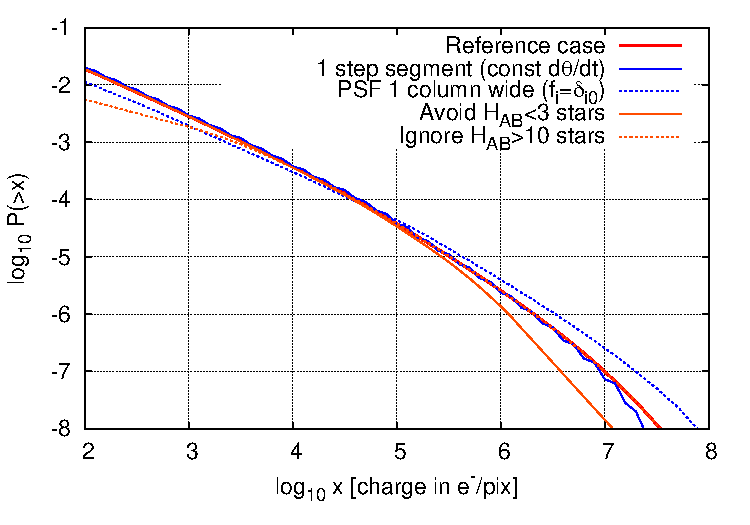
\includegraphics[width=5in]{Plots/slew_compare.pdf}
\caption{\label{fig:slewcompare}Comparison of stimulus levels predicted
under different assumptions and approximations. The vertical axis
shows the log probability to exceed a given stimulus level during a
slew of 0.4 degrees (a step along the short axis of the field,
executed frequently during the HLS). The thick red line indicates
reference assumptions. The solid blue line treats the slews as being
at constant $\dot\theta$. The dashed blue line approximates the PSF as
1 column wide (all the flux from the star is concentrated in the
central column). The orange lines show what happens if bright ($H_{\rm
AB}<3$) or faint ($H_{\rm AB}>10$) stars are excluded from the model.}
\end{figure}

\begin{figure}
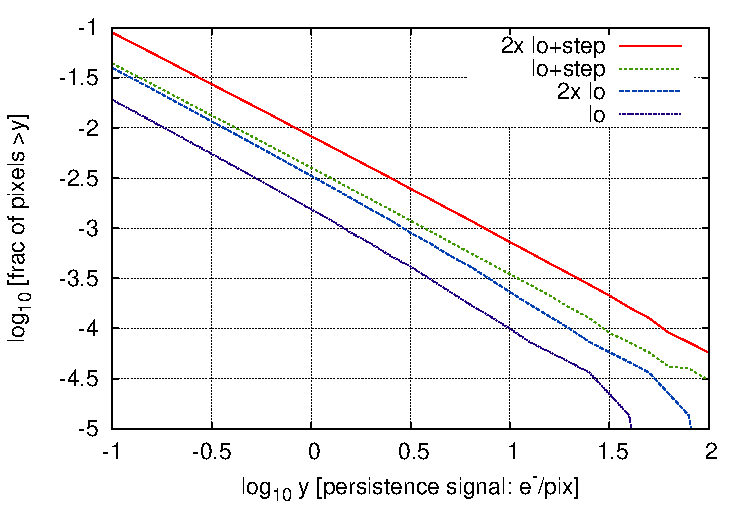
\includegraphics[width=5in]{Plots/sp_cdf.pdf}
\caption{\label{fig:sp_cdf}The cumulative distribution function of slew-induced persistence in the HLS imaging survey, $P(>y)$.
The persistence signal $y$ is estimated in electrons per pixel; the decaying persistence curve is integrated over a 160 s. Several persistence models are shown, including the ``lo'' case (typical of the development detectors), and a ``lo+step'' case (including an order of magnitude step at saturation, as seen in portions of some detectors). This figure has not been updated yet to go from the 6-year to the 5-year observing plan, although we expect only minor differences.}
\end{figure}

After negotiating with the Project, we settled on a mitigation strategy for slew persistence that involved saving the spacecraft orientation information from the Attitude Control System (ACS), using this to predict the locations of persistence from bright star streaks, and masking $\pm2\sigma$ on either side of these streaks. Unmasked streaks are simply accepted as part of the systematic error budget. Their impact on shape measurement is based on an analytic result derived by our SIT and tested against Monte Carlo simulations:
\begin{equation}
\Delta \gamma_1 + i\Delta \gamma_2 = \frac{M\Omega_{\rm
max}\sigma_{\rm n}^2 R^4}{2F^2N_{\rm ind}\,{\rm Res}} f_{\rm scale}
f_{\rm aniso},
\label{eq:dg}
\end{equation}
where $\Delta\gamma_{1,2}$ are the two components of spurious shear; $M$ is a margin factor; $\Omega_{\rm max} = 421.3$; $\sigma_{\rm n}^2$ is the variance of the persistence image; $R$ is the radius of the galaxy in pixels; $F$ is the signal from the galaxy in electrons per exposure; $N_{\rm ind}$ is the number of {\em independent} exposures of the galaxy\footnote{This may be less than the total number of exposures of the galaxy, since slew persistence from successive exposures will be correlated.}; Res is the galaxy resolution factor \cite{Bernstein2002}; $f_{\rm scale}$ and $f_{\rm aniso}$ are factors $\le 1$ describing the scale dependence and anisotropy of the persistence power spectrum (defined to be 1 in the worst case).

The results of this study -- shown in Figure~\ref{fig:slew_results_oct16} -- are promising, given the top-level systematic shear budget of $2.7\times 10^{-4}$ and that the modern detectors typically show ``lo'' or (in some regions) ``lo+step''-like behavior, rather than the much larger persistence characteristic of the WFC3-IR model (third column). The masking algorithm will continue to be revisited as part of the mission optimization. However, the small number of masked pixels led the FSWG to conclude that a dark shutter that operated during every slew was not required for the WFIRST HLS.

\begin{figure}
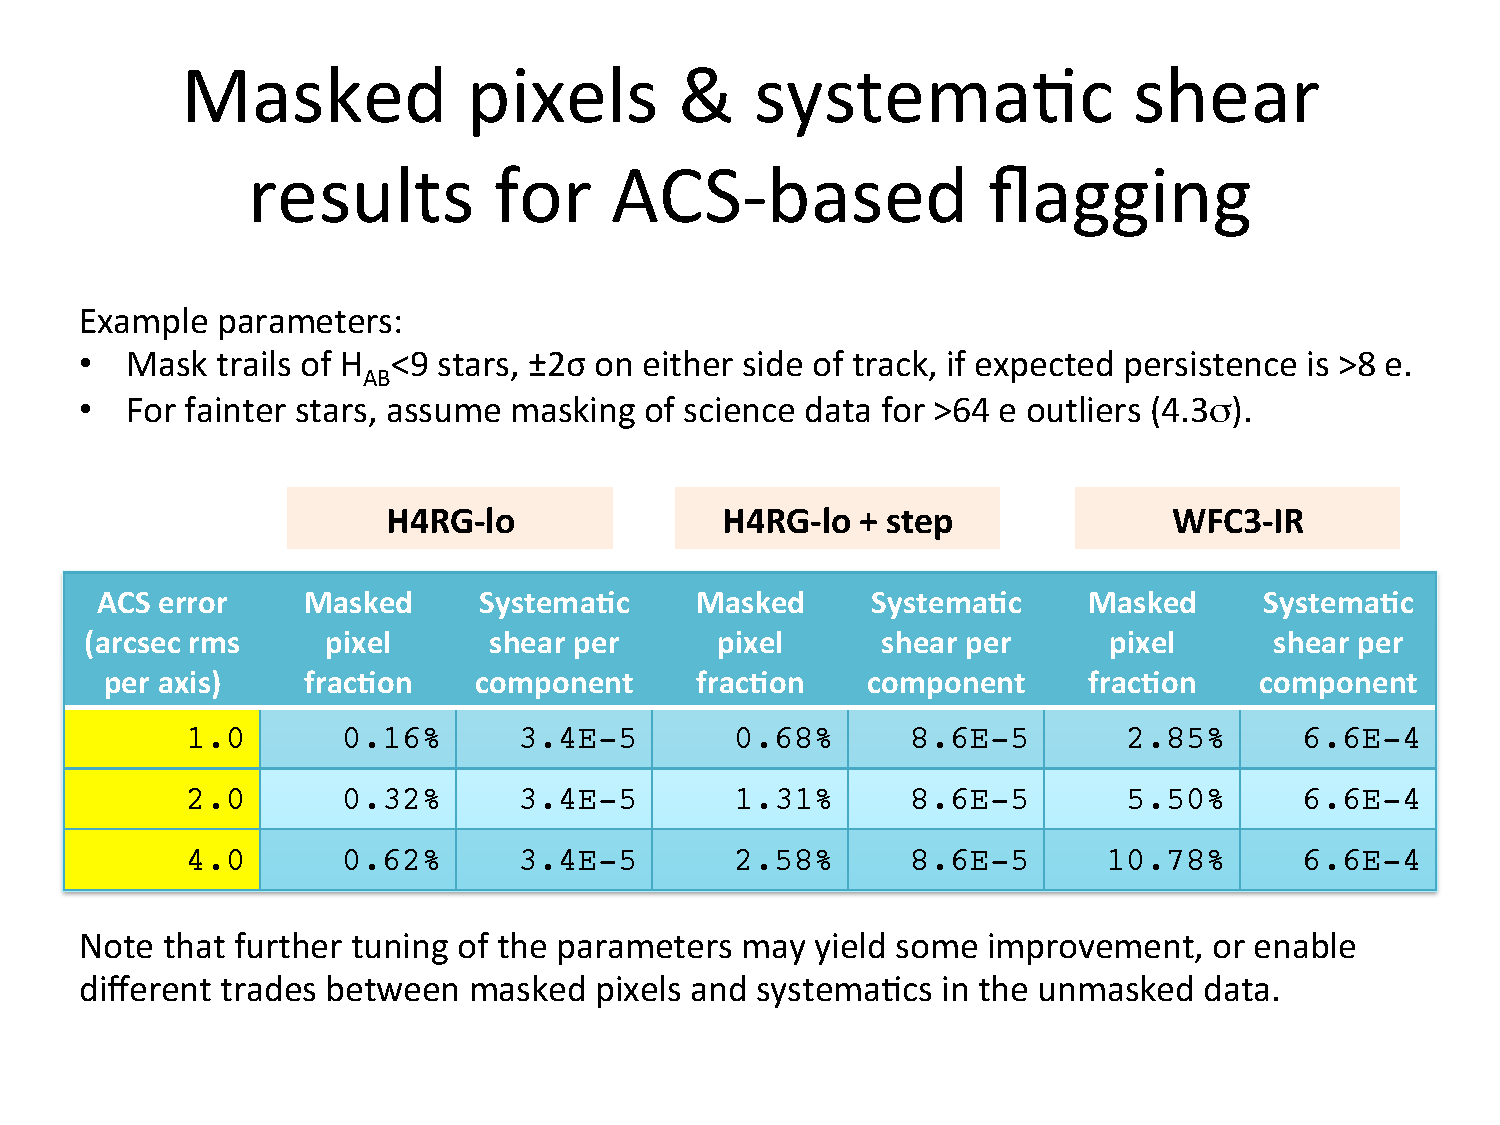
\includegraphics[width=5in]{Plots/slew_results_oct16.pdf}
\caption{\label{fig:slew_results_oct16}The outcome of the October 2016 slew persistence study. This shows the masked pixel fraction and the predicted systematic shear due to unmasked streaks as a function of both the persistence model and the accuracy of pointing information.}
\end{figure}

We carried out a related study, also using Eq.~(\ref{eq:dg}) and related machinery, to assess how well we need to know the dark current for WFIRST. Dark current measurements without a dark filter are possible, e.g.\ via median algorithms that combine many exposures from a survey, but are subject to: (i) a degeneracy in which the ``true'' sky brightness is unknown and hence the zero level of the dark current cannot be established, and (ii) possible correlated errors from imprinted celestial sources. The requirements, as derived in the appendix to the calibration plan, are:
\begin{list}{$\bullet$}{}
\item The error in the dark current + bias determination in a 140 s
HLS imaging exposure shall be no more than $0.0096f_{\rm corr}^{-1/2}$
e/p/s (uncorrelated part) or $0.0017 f_{\rm corr}^{-1/2}$ e/p/s
(imprinted celestial sources).
\item The error in the dark current + bias determination in a 297 s
HLS spectroscopy exposure shall be no more than $0.0059 f_{\rm
corr}^{-1/2}$ e/p/s (uncorrelated part) or $0.00072 f_{\rm
corr}^{-1/2}$ e/p/s (imprinted celestial sources).
\end{list}
Here ``$f_{\rm corr}$'' denotes the factor by which we plan to correct biases induced by errors in the dark current map (we normally choose $f_{\rm corr}=1$ to be conservative). The requirements are traceable to additive shear biases from non-circular imprinted celestial sources; multiplicative shear biases as the noise in the dark current map results in e.g.\ galaxy centroids getting ``pulled'' toward pixels whose measured dark current fluctuates below the true dark current of that pixel; and Eddington-like biases for sources detected in the GRS. While the semi-analytic estimates in the calibration plan based on source counts suggest that the HLS imaging requirement can be met without a dark filter, our SIT and the Calibration Working Group had concerns about possible degeneracies in the self-calibration procedure that can only be addressed by a detailed simulation. Moreover, the approach requires empty space in the images, which we will not have in the case of grism spectroscopy. As the imaging exposures are shorter than the spectroscopy exposures, this would require dedicated long imaging exposures (of HLS spectroscopy exposure length) just for the purpose of self-calibrating the dark. Due to sky Poisson noise, we would need many of these images -- our Feburary 2017 estimate was for $N=73$ exposures, which, if done every week, would consume 4\%\ of the wall clock time. In light of these and other issues, the Calibration Working Group recommended that WFIRST maintain the dark filter.

\subsubsection{Calibration plan}

\textcolor{red}{Write this part.}

\subsubsection{Detector characterization}

\textcolor{red}{Write this part.}

\comment{
Achieving a uniform photometric calibration of the survey is an essential requirement
for achieving the scientific goals of WFIRST, since calibration variations on large
scales can swamp the cosmological signals and make dedicated photo-$z$ calibration
fields unrepresentative of the whole survey.
Our calibration requirements and
strategy development will be led by Co-I Padmanabhan, the chief
architect of the ``uber-calibration'' method used for the SDSS \cite{Padmanabhan2008};
members of our team also have experience designing calibration strategies for
Euclid and LSST.  Co-I Capak is an active member of the Euclid calibration team. Co-I Lupton plays a
key role in designing LSST and HSC calibration strategies.
Using our simulations and forecasting tools, we will determine both
absolute and relative calibration requirements for the survey as a function
of angular scale on the sky. Based on these requirements, we will
define a calibration plan for WFIRST, including overlapping regions
for self-calibration over the entire survey and repeated fields or use of
the microlensing survey data for small scale calibration (e.g., flat fields
and intra-pixel response).  We will also define methods and metrics for
tracking the photometric stability and calibration quality
across the survey.
We will determine formats for making the calibrations and calibration
error maps publicly available to enable related analyses.
We will pay special attention to the relation of the photometric calibration
strategy to instrument design, including the impact of field-dependent bandpass
variations and NIR detector effects such as persistence and rate-dependent nonlinearity.
We will track which such effects can be measured internally to the WFIRST data, and
when dedicated observing modes might be needed (such as observations of the sky with
an internal illumination source also on). The latter considerations will feed into
the observing strategy and hardware requirements.
}

\subsection{Photometric Redshifts}
\label{sec:wl_calibration}
%================================================
\Auth{Peter, Shooby, Dan}

Accurate photo-$z$s are crucial to all WFIRST probes of
dark energy. We plan to combine calibrations of the color-redshift relation
\cite{Masters2015} and cross-correlation techniques to achieve the
required photo-$z$ performance. These will be supplemented by
consistency checks such as the expected level of WL cross-correlations
for sources in different photo-$z$ bins.
Our team is actively developing the color-redshift mapping for WFIRST
(supported by WFIRST Preparatory Support (WPS); PI Capak),
with initial tests demonstrating a path
to meeting the WFIRST requirements on photo-$z$ bias. Our team has worked with NASA HQ
to allow the NASA Strategic Keck Proposals to obtain the required spectra.
A key piece of the proposed work will be carrying out these spectroscopic surveys.
Cross-correlation methods \cite{2008PhRvD..78d3519H, 2008ApJ...684...88N, Menard2013, Newman2015} require
spectroscopic overlap and rely on assumptions about the bias of galaxies. We
will determine the applicability of these methods and their implications for
survey design. We also plan
to investigate promising new methods of photo-$z$ inference \cite{Bordoloi2010, Jasche2012, Benjamin13}
as additional consistency checks.

Our team will refine the performance estimates and calibration data requirements for each of
these photo-$z$ methods. This will include studying the impact on WFIRST operations
(e.g., incorporating observations of spectroscopic calibration fields in the observing plan).
Co-I Capak will lead the photo-$z$ effort, with support from other team members (Mandelbaum, Hirata,
Hudson, Jain, Eifler, Krause, Miyatake) who have extensive experience
using photo-$z$ calibration techniques for WL applications with SDSS
(e.g., \cite{2012MNRAS.420.3240N,2008MNRAS.386..781M}),
Canada-France-Hawaii Telescope (CFHT), DES and HSC survey data.


%{\bfseries C.H.: Need uniform ``primary/secondary/tertiary'' nomenclature. Also discuss photometric calibration requirements.}

%\subsection{Cosmological Forecasting, Methodology Development, and Cosmological Simulations}
\subsection{Cosmological Forecasting, Simulations, and Methodology Development (D2, D8, D9)}
\label{sec:wl_methodology}
%=========================================================================
%\Auth{David W, Tim, Elisabeth, Rachel B, Alina, Bhuvnesh}


\subs{Forecasting.}
Cosmological forecasting plays
an essential role in connecting strategies and requirements defined at
the instrument and observation level to WFIRST's top-level science goals.
Co-Is Bean, Hirata, Padmanabhan, Wang and Weinberg have been
involved in the forecasting for the WFIRST reports and
for cosmological surveys and space missions in general.
One of our early activities will be to develop a forecasting
framework for WFIRST building on Eifler \& Krause's \CoLi, incorporating all of the dark
energy probes from the HLS Imaging, Spectroscopy, and Supernova surveys.
We will incorporate the impact of the leading observational and theoretical systematics
through ``nuisance parameters'' that can be marginalized over in cosmological
parameter estimates.  This framework will be much more thorough
than the one used for the SDT reports, and it will enable complete
flow-down and flow-up analyses between the instrument, strategy, and
software requirements and the expected cosmological performance of
WFIRST.  We will initially use analytic approximations for error covariance
matrices and the dependence of observables on model parameters.  We will
steadily update these approximations using the simulations described below.
For cosmic shear, we will extend existing work on the WL bispectrum
(e.g., \cite{Kayo2013,Fu14}), which should
produce complementary constraints to the power spectrum and may have
similar statistical power given the high source density expected in
HLS Imaging.  Figure~1 illustrates the application of \CoLi\ to WFIRST
multi-probe forecasting.

\subs{Cosmological simulations.} As emphasized in SDT15, WFIRST will improve the statistical precision
of cosmic expansion and structure growth measurements by factors of $5-50$
compared to current data, and will require commensurate improvements in modeling the
lensing and clustering signals  and the astrophysical contaminants thereof.
We will  devote significant effort to modeling the nonlinear regime via a combination of numerical
simulations, perturbation theory, and empirical measurements, to
 address issues such as baryonic effects on matter clustering
\citep{Zentner2013,VanDaalen2014}; the
validity of the Born approximation \citep{Schafer2012}; and galaxy intrinsic
alignments \citep{Hirata2004,Laszlo2011,Krause2015}.
We will develop analysis strategies that take advantage of
our methodological improvements and marginalize over remaining uncertainties.
The computational requirements for cosmological simulations will increase
significantly in the years just prior to launch. Where these resources will
be sourced from is currently an unsolved issue that is being investigated at
the project level. Co-I Kiessling has been part of this effort at the request of
the project and she will be responsible for leading
the team efforts to quantify computing requirements beyond FY20.
% and to develop techniques to reduce them.
%
% RM took a bunch of long specific sentences and made this more general one.
%For cosmic shear, we will develop
%``self calibration'' strategies to eliminate biases and mitigate statistical
%losses from uncertainties in shear calibration and \photoz\ error
%distributions.  These strategies will be developed in concert with
%and informed by the methods and tests discussed previously in
%\S\ref{sec:wl_requirements} and~\ref{sec:wl_methodology}.
%We will use cosmological N-body simulations and hydrodynamic
%simulations to predict non-linear matter clustering at the accuracy
%needed for WFIRST modeling, including the impact of realistic
%treatments of baryonic physics (see, e.g., \cite{Zentner,VanDaalen,Etc}).
%We will apply ray tracing to cosmological simulations to test
%for biases such as due to the ``Born approximation'' typically used in weak
%lensing analysis, and to calibrate any necessary corrections.
%We will use hydrodynamic simulations, perturbation theory calculations,
%and empirical information to sharpen predictions of galaxy intrinsic alignment,
%one of the main theoretical systematics for cosmic shear.

%\textbf{Bhuv: The two paras below describe a very broad program. If not essential, perhaps better to make it shorter and less sweeping. Also, is the connection to image simulations ok?}
%Our methodology development and tests will make heavy use of cosmological
%simulations.
Most of our work will use large-volume $N$-body simulations (gravity only) in concert
with statistical recipes or semi-analytic models for assigning
galaxies to dark matter (sub-)halos. A large set of such simulations ranging in size from tens of billions to a trillion particles already exists. These will be made available to the collaboration by collaborator Heitmann and will be augmented over time with more simulations as needed.
We will use hydrodynamic simulations
of smaller volumes, provided by collaborator Yoshida, for targeted investigations such as the impact of
baryonic physics on the matter power spectrum or as a realistically
complicated test of non-linear galaxy bias models.
From the $N$-body simulations we will produce mock galaxy catalogs
both in fixed redshift cubes and in light cones with realistic survey
geometry and redshift evolution.
We will use these mocks to understand the effect of observational complications
(survey geometry, variable depth and completeness, etc.) on WL and clustering
measurements and to provide realistically clustered inputs for the pixel-level
simulations described earlier.

% C.H. -- I would really like this but it's very ambitious and not clear that it is
% higher priority than subsets of the HLS simulated at very high fidelity.
% By the end
%of the 5-year investigation period, we aim to produce several complete
%realizations of the full pixel-level HLS data set.

%The overall cosmological simulation effort is large, but many ambitious
%dark energy experiments face a similar challenge.
Our team includes
Co-I Kiessling and collaborators (Heitmann, Takada, Yoshida) who are leading similar efforts
for Euclid, Subaru HSC and PFS, DES, DESI and LSST. In \S
\ref{sec:fac_equip} we describe the computing facilities that will
enable these computations.
%By 2020, advances in computing will make it possible to run larger numbers of simulations, or explore more parameter space at a given size and resolution.
We will publish papers documenting our methodology development and
will simultaneously release the associated simulations.
This growing library of publicly available simulations will encourage
the broader community to develop analysis strategies that will
ultimately be applied to WFIRST (and other surveys).
%While we expect major advances over
%the 5-years of this SIT, we do not expect to solve all of the modeling
%challenges in this period.  One of our deliverables will be a list of remaining (post-CDR) tasks
%to address the remaining modeling uncertainties.

%\setlength\intextsep{-2pt}
%\begin{center}
%\begin{wrapfigure}{r}{1.0\textwidth}
\begin{figure}[!t]
 \begin{boxedminipage}{1.0\textwidth}
 \begin{center}
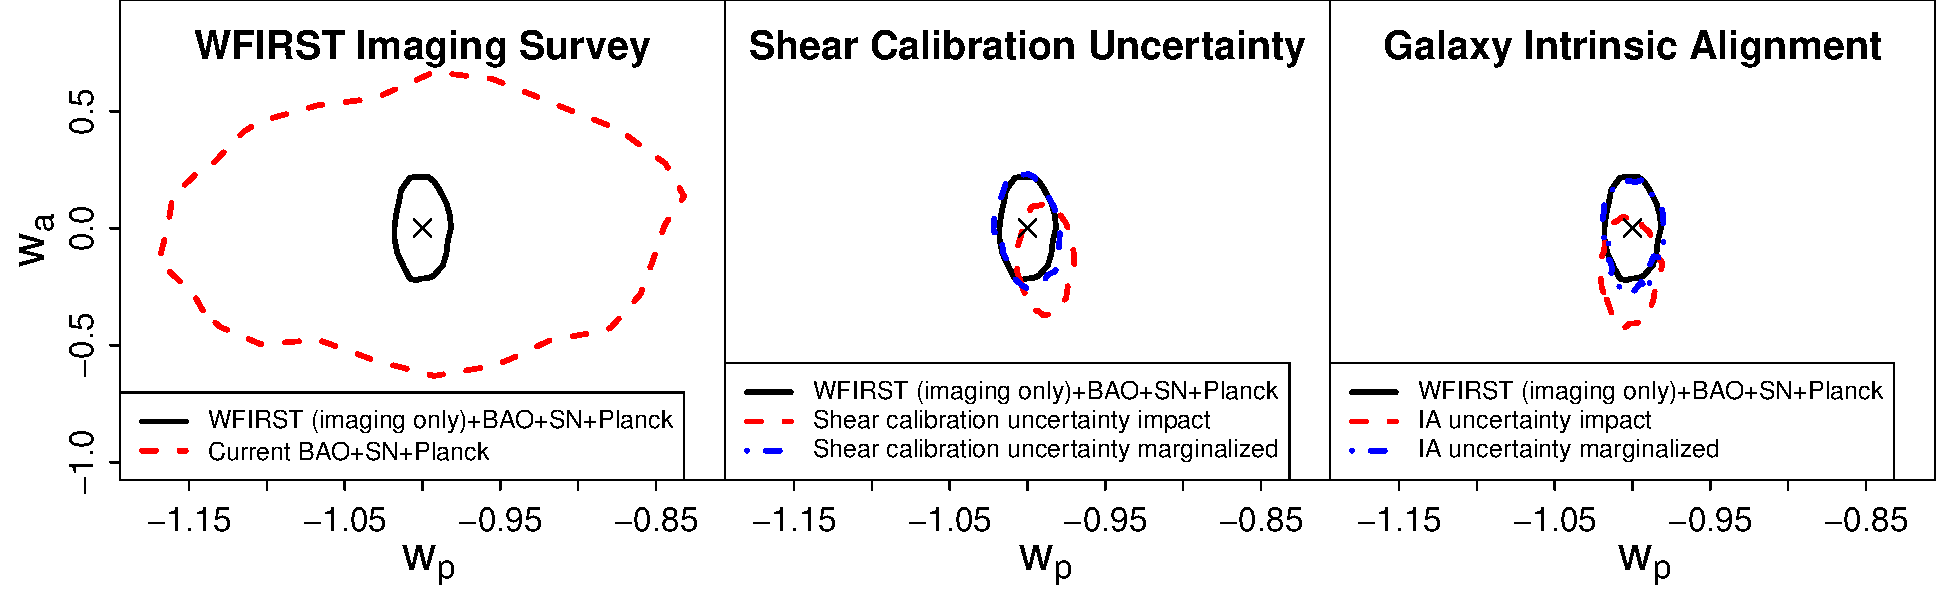
\includegraphics[width = \textwidth]{Plots/WFIRST_combi_forecasts.pdf}
\label{fig:WLsys}
 \end{center}
\vspace{-1.25cm}
\caption{\footnotesize{\CoLi\ forecasts of constraints on the dark energy equation-of-state
from combining current CMB+BAO+Supernovae (SN) data with anticipated WFIRST WL, GGL, projected clustering, cluster number counts, and cluster weak lensing measurements.
We adopt a flat universe with a DE equation of state
$w(z)=w_0+w_a[1-(1+z)^{-1}]$, with the $x-$axis showing the
value of $w$ at the pivot redshift ($z_p$) where it is best constrained by this data combination.
The left panel shows the improvement from WFIRST imaging data with statistical errors only.
In the middle panel, red contours show the effect of an uncorrected shear calibration error
of magnitude 0.004, while blue contours show the result with the same calibration error
after marginalizing over five shear calibration nuisance parameters with Gaussian priors of
width 0.002. The right panel shows a similar example for an astrophysical systematic,
the presence of galaxy intrinsic alignments (see \cite{Krause2015} for details). In both cases, marginalization removes the systematic error without significantly increasing the statistical uncertainty.
}}
%\begin{center}
\end{boxedminipage}
\end{figure}
%\end{wrapfigure}
%\setlength\intextsep{0pt}

\subs{Galaxy-galaxy lensing.} The combination of GGL with galaxy clustering
is an alternative route to extracting cosmological constraints from
an imaging survey.  Systematics are significantly different from those
affecting cosmic shear analysis, and theoretical studies suggest that
the statistical power is comparable \cite{Yoo2012}.  The need to mitigate systematics
favors a joint modeling approach to cosmic shear, GGL, and galaxy clustering,
which requires devising and testing models of non-linear galaxy
clustering and its dependence on redshift, building on studies such as
\cite{Yoo2006,Baldauf2010,Cacciato2013,Mandelbaum2013,Coupon15,More2015,Zu2015} and
including the possible impact of ``assembly bias'' connected to halo
formation histories.
We will include GGL in our cosmological forecasting framework
and identify any GGL-specific requirements distinct from those
tied to cosmic shear.

\subs{Clusters.} Our efforts in cluster analysis methodology will parallel those for
cosmic shear and GGL, facing many of the same issues but in the
(somewhat simpler) high mass halo regime. Co-I Weinberg
will lead the cluster effort with support from collaborators Rozo and
von der Linden.  While the WFIRST data set presents some
unique issues, we will draw extensively on the machinery being developed for
DES by Rozo, which follows the broad strategy laid
out in chapter 6 of \cite{Weinberg2013}, and for LSST, described in \cite{LSSTDESC12}.

The first branch of the cluster effort will focus on the identification
and characterization of clusters in WFIRST+LSST (or WFIRST+HSC) imaging.
This optical+NIR combination will lead to the best statistical precision,
since optical/IR selection can select clusters (at typical redshifts
$z \sim 0.5-1.5$) down to mass thresholds significantly lower than
X-ray or Sunyaev-Zeldovich detection; we expect $\sim 40,000$ clusters in the HLS
with masses $>10^{14}M_\odot$.
Building on DES methodology
\cite{Rykoff2014}, we will design and test (in simulations) prototype cluster finders for
WFIRST+LSST data.
Among the issues we will address are: completeness and contamination
of the cluster catalogs as a function of redshift and richness; biases
in estimated richness or cluster redshift; expected scatter between
richness and halo mass; accuracy of galaxy photometry in cluster regions;
accuracy of shear measurement in cluster regions; reliable separation
of foreground, member, and background galaxy populations for weak
lensing analysis; and ellipticity- or orientation-dependent
cluster selection.

A second branch recognizes WFIRST's unique potential for calibrating
cluster mass-observable relations at $z\gtrsim1$ via weak lensing.
Cluster-galaxy lensing (CGL, e.g.,
\cite{Sheldon2009,VonDerLinden2014}) is the method of choice for all
cluster surveys overlapping weak-lensing surveys, but requires
sufficient number densities of galaxies behind the clusters with
accurate photo-$z$s.  For cluster mass calibration at $z\gtrsim1$,
space-based shear measurements and photo-$z$s from the combination of
LSST and deep NIR photometry, such as delivered by WFIRST, are
therefore necessary. Calibrating cluster mass-observable relations
furthermore benefits tremendously from the availability of
multi-wavelength mass proxies (e.g. \cite{Wu2010}), hence we will
consider the synergies with X-ray (eROSITA) and SZ (Planck, AdvACT,
SPT-3G, CMB-S4) measurements, with special attention to the impact on
survey footprint placement.  We will also investigate the potential for HLS-CMB cross-correlations to extract the kinetic Sunyaev-Zeldovich signature to constrain dark energy, gravity and and neutrino mass sum \cite{Mueller2014a,Mueller2014b}.  Magnification of special galaxy subsamples can provide a cross-check on
the shear-based lensing effort (e.g., \cite{Hildebrandt13}).

For modeling methods, we will develop a comprehensive approach that combines CGL and cluster-galaxy cross-correlations
to extract cosmological information from fully non-linear, trans-linear,
and linear scales, extending and unifying methods based on the
cluster mass function (e.g., \cite{Rozo2010}, \cite{Mantz2015}), cluster mass-to-light
or mass-to-number ratios \cite{Tinker2005,Tinker2012},  large scale
cluster-mass correlations \cite{Zu2014}.
We will test the robustness of these methods to all of the observational
effects listed above.
For our cosmological forecasting, we will integrate clusters with our
\CoLi\ treatment of WL and the GRS to account for
correlated statistical errors (from large scale structure in the HLS
survey volume) and common systematics (shear calibration, photo-$z$ errors).

\subsection{Systematics Testing and Mitigation (D8)}
%===================================

Achieving WFIRST's precision cosmology goals requires eliminating systematic biases
while minimizing statistical losses, and {\it demonstrating} that biases have been
removed.  We will develop a 3-pronged approach to this challenge.

\subs{Marginalization.}
As illustrated in Figure~1, a general strategy for both instrumental and astrophysical
systematics is to describe their possible impact by nuisance parameters and
marginalize over these in cosmological analysis.  Important elements in making
this strategy effective are:
(i) devising concise templates that describe the systematics with minimal
numbers of parameters;
(ii) setting realistic priors on nuisance parameters;
(iii) combining multiple observables that can break degeneracies.
We will develop this approach for treating observational effects,
particularly shear measurement systematics and photo-$z$ biases,
and astrophysical effects, particularly the impact of baryons
on the matter power spectrum \cite{jzl2006,rzk2008,dsb2011,shs2011}
and galaxy intrinsic alignments (IA).  For the observational effects,
we will use our simulations (\S 4.1) and photo-$z$ investigations
(\S 4.2) to design templates and determine appropriate priors.
For the astrophysical effects, we will draw on our team's extensive
experience with analytic and numerical modeling of IAs
\cite{Hirata2004,Mandelbaum2006,Hirata2007,Mandelbaum2011,Heymans13,Kiessling2015,
Kirk2015,Singh2015,Tenneti2015}
and on the work of Eifler and Krause in incorporating baryonic and
IA effects into cosmological WL analysis \cite{Laszlo2011,Kirk2011,Eifler2014,Krause2015}.
This will include the principal components approach, which allows one to
marginalize out the directions in observable space that are most sensitive
to the choice of prescriptions for baryonic physics in simulations
\cite{Eifler2014}.
Cosmic shear, GGL, CGL, and galaxy clustering each respond differently
to these systematics, so we anticipate that joint analyses will allow
much tighter constraints on both systematics and cosmology than any
probe in isolation.


\subs{Systematics maps.} A second approach to identifying and removing
observational systematics is to cross-correlate the signal being
measured with maps of possible systematic effects, such as stellar
density, PSF size, or Galactic extinction (e.g., \cite{Ross2012}).
These methods both measure the impact of systematics and provide a template for removing
them.  We will devise a system of such methods for WFIRST WL and
galaxy clustering measurements and test their efficacy on our simulated
data sets.  This effort will be led by Co-Is Ho and Padmanabhan, who
developed such approaches for their analyses of large scale galaxy
and quasar clustering in the SDSS \cite{Ho2015,Padmanabhan2007}.

\subs{Null tests, internal consistency, and external data sets.}
WL analyses must be validated using internal tests that the measurements
should pass for any set of cosmological parameters
but may fail in the presence of systematics (e.g., \cite{Jarvis2015}).
For example, the cross-correlation between
PSF-corrected galaxy shapes and star shapes should be consistent with zero,
many statistics associated with $B$-mode shear (e.g., \cite{Eifler2008}) should vanish,
and consistent cosmological results
should be obtained when using the largest or smallest 50\%\ of the source galaxies.
Drawing on our team's experience with other surveys, we will ensure that
there is a coherent pipeline for carrying out these standard tests on WFIRST
data, including the many consistency tests enabled by having shape
measurements in multiple bands.
We will pay close attention to tests that make use of unique properties of WFIRST data;
for example, comparison of
shapes measured on subsets of an exposure with multiple non-destructive reads would test for
the impact of detector non-linearities.

Cross-correlations with external
imaging and spectroscopic surveys (Kilo Degree Survey (KiDS), HSC, DES, PFS, DESI, LSST, Euclid)
offer multiple opportunities for improving the HLS analysis, including
photo-$z$ calibration and tests for shear systematics.
For example, the cross-correlation of WFIRST and LSST shapes
will evade additive systematics that impact
only one or the other survey, e.g.,
those coming from the atmosphere for LSST or from
detector effects specific to WFIRST.
Other validations can be performed using surveys that measure similar quantities as the
HLS but using different techniques, such as cluster masses estimated  via CMB lensing.
We will investigate a variety of possible tests, evaluate
the hardware and operations implications (e.g., footprint overlap,
joint data management), and ensure that they are represented in the FSWG process.


%Developing and implementing sophisticated systematics mitigation strategies will be
%a key research area to prepare for a successful WFIRST mission. In principle, systematics
%mitigation techniques can be separated into parametric and non-parametric categories.
%Parametric descriptions of systematics rely on observations from external data sets,
%simulations, and/or theoretical models; their functional form reflect the physical concepts
%that, to the best of our knowledge, describe the systematics. Uncertainties are described
%via freedom in so-called nuisance parameters and identifying methods to impose stringent
%priors on these nuisance parameters is pivotal to extracting cosmological information.

%In the absence of knowledge on the parameterization of systematics one has to resort to
%non-parametric descriptions, i.e., allow for sufficient freedom in the model. This will
%heavily diminish cosmological constraining power, which again stresses the importance for
%a carefully designed effort to obtain prior information on systematics. In the following
%we describe the current state of the art for parametric systematics templates and our plans
%forward in improving these models. The photometric redshift error testing/mitigation
%strategy is sufficiently complex that it is discussed separately (\S\ref{sec:wl_calibration}).

%\subs{Nonlinear structure growth and baryonic effects on WL.}
%Although early work \citep{jzl2006,rzk2008} suggested a small impact on cosmic shear due to baryonic physics,
%\cite{dsb2011} find that when including AGN feedback, baryons can suppress the matter power spectrum by 30\% at $k=10$
%h/Mpc, 10\% at $k=1$ h/Mpc, and 1\% at $k=0.3$ h/Mpc.
%Subsequent work \cite{shs2011} showed large biases in cosmological parameters if baryons were neglected, and
%propose the use of a halo model-based mitigation scheme. We will use the simulations described above to more carefully characterize the uncertainties
%due to baryonic effects, and to confirm the efficacy of mitigating them empirically by profile fitting or using principal components analysis. Our team includes key players (Eifler, Krause)
%in the development of these mitigation strategies \citep{Eifler2014}.
%We will also estimate the residual uncertainties and feed this into parameter forecasts.

%\subs{Shear systematics.}
%Systematic errors in shear measurement can take many forms.  Among the simplest are
%multiplicative biases that lead to a scale-independent (though redshift-dependent) rescaling of the cosmic shear signal
% or additive biases
%that can often be treated as linear in the PSF anisotropy \cite{Mandelbaum2015}
%and detected fairly simply using null tests.  However, there are other shear systematics
%that can have interesting scale-dependence, such as the effects of PSF modeling errors,
%detector effects, etc. We will use the preliminary simulation
%software described in Sec.~\ref{sec:wl_requirements} to forecast these systematics, derive hardware
%requirements to suppress them, and derive templates that can be used to search for specific systematics in the data.
%The more complicated systematics (e.g., deblending, crowding-induced selection effects) will also
%require the more realistic simulation tools to be developed by the WSC.
%While many of the approaches to these systematics are generic, and our team brings experience
%from many past and present WL surveys (CTIO, SDSS, DES, HSC), we will pay special attention to
%issues unique to the WFIRST optical configuration and detectors.

%\subs{Intrinsic alignments.}
%Template marginalization to remove IAs will involve
%a joint analysis of tomographic shear-shear, galaxy-shear, and galaxy-galaxy cross-correlations \citep[e.g.,][]{Joachimi2010}.
%Building templates for the effect of IAs
%will involve a combination of analytical and simulation models,
%and observations to place priors on model parameters \cite{Kirk2015,Kiessling2015}.
%Our team members have key experience in the theory (e.g., showing that IAs
%contaminate shear correlations between different redshifts \cite{Hirata2004}),
%observations \cite{Mandelbaum2006, Hirata2007, Mandelbaum2011, Singh2015}, and interpretation of simulations \cite{Kiessling2015,Tenneti2015}.
%We must extend these approaches for WFIRST due to its NIR observations and sensitivity to smaller and fainter
%galaxies than current WL surveys.
%
% C.H. I think an internal consistency test ("X=Y to within errors") is the same as a null test
% ("X-Y=0 to within errors") ... just sometimes we formulate the tests in different ways ...
%
%\subs{Internal consistency and null tests.}
%WL analyses must be validated using internal tests in the data that should pass for any set of cosmological parameters
%but may fail in the presence of systematics (e.g., \cite{Jarvis2015}).
%For example, the cross-correlation between
%PSF-corrected galaxy shapes and star shapes should be consistent with zero,
%many statistics associated with $B$-mode shear (e.g., \cite{Eifler2008}) should vanish,
%and consistent cosmological results
%should be obtained when using the largest or smallest 50\%\ of the source galaxies.
%These tests have differing sensitivities to technical and astrophysical systematics.
%They are standard across surveys, so our main priority
%will be to ensure there is a coherent pipeline for carrying these standardized tests out
%on WFIRST data. However, we will pay close attention to tests that make use of unique properties of WFIRST data;
%for example, comparison of
%shapes measured on subsets of an exposure with multiple non-destructive reads would test for
%the impact of detector non-linearities.

%%%\begin{comment}
%%%\paragraph{Photometric Redshift Uncertainties}
%%%Calibration and validation of photometric redshifts (photo-z's) in the HLS is essential to
%%%achieve the weak lensing and cluster cosmology goals. The combination of WFIRST and LSST
%%%photometry will enable photometric redshift estimates out to redshift $\sim$3. Nevertheless
%%%uncertainties in the passage of the Lyman and Balmer breaks through the broad band filters
%%%leads to scatter between the estimated photo-z and the true redshift, and in rare cases to
%%%catastrophic outliers due to confusion between the breaks. Dark energy information via
%%%lensing tomography and cluster masses degrades due to scatter and bias in the photo-z
%%%estimates. As shown in the WFIRST report, a scatter of $0.06(1+z)$ is achievable for the
%%%HLS lensing galaxies, but this needs careful validation with realistic mock galaxies.
%%%Systematic biases well above 0.1\% in the mean redshift of tomographic bins can significantly
%%%degrade dark energy constraints, thus setting a tight requirement on photo-z calibration.
%%%Minimization strategies to be pursued include calibration with spectroscopic data and
%%%self-calibration based on the clustering of galaxies and via tomographic lensing measurements.
%%%An example of the latter is the use of the redshift variation of the galaxy clustering and
%%%galaxy-galaxy lensing signal (possibly with CMB lensing providing additional information)
%%%to place priors on the parameters that characterize the uncertainties in the photo-z
%%%distribution. Mandelbaum, Hirata, Jain, Eifler, Krause and other members of our team have
%%%modeled and employed photo-z calibration techniques with SDSS, DES and HSC survey data.
%%%We will extend and test the applicability of techniques employed for ongoing surveys via
%%%mock catalogs representing the HLS.
%%%\end{comment}

%\subs{External datasets.}
%%The two sentences below are repeated in Section 8.
%External imaging and spectroscopic surveys (KIDS, HSC, DES, PFS, DESI, LSST, Euclid)
%provide several opportunities for improvements in the HLS analysis, such as in the calibration
%of photo-$z$s and shears. In addition, these surveys provide redundant measurements that can
%be used to validate the analysis of both WFIRST and the other surveys.
%In addition to cross-checking the tomographic shear power spectra (which should be consistent after correcting
%for the different shapes of the redshift bins), direct cross-correlations of the data
%provide a powerful internal test.
%For example, the cross-correlation of WFIRST and LSST shapes
%will evade additive systematics that impact
%only one or the other survey, for example those coming from the atmosphere for LSST or specific detector effects
%for WFIRST.
%%We will identify additional such tests and implement them
%%on mock catalogs with the characteristics of the HLS and surveys from LSST and perhaps
%%other telescopes.
%Other validations can be performed using surveys that measure similar quantities as the
%HLS but using different techniques, such as cluster masses estimated  via CMB lensing.
%Our end goal will be to understand the hardware and operations implications (e.g., footprint overlap,
%joint data management) of these tests and ensure that they are represented in the FSWG process.


%\vspace{-0.15in}
%=============================================
\section{Galaxy Redshift Survey Investigation}
%=============================================
\label{sec:gc}
 %1-2 paragraph overview of science goals.  BAO, RSD, other applications.
 %SDT2015 as starting point.


%\begin{tcolorbox}[width=\textwidth,colback={mypink3},title={With true corners},outer arc=0mm,colupper=white]
%     Test
%     %%\includegraphics[scale=0.5]{frogimage.png}
%\end{tcolorbox}

%\begin{tcolorbox}[width=\textwidth,colback={coralpink},outer arc=0mm,colupper=white]
%     Test
%     %%\includegraphics[scale=0.5]{frogimage.png}
%\end{tcolorbox}

%\begin{textbox}[h]\section{SIDEBARS}
%Sidebar text goes here.
%\subsection{Sidebar Second-Level Heading}
%More text goes here.\subsubsection{Sidebar third-level heading}
%Text goes here.\end{textbox}


% Summary Points

% Future Issues
The defining goal of HLS spectroscopy is to derive constraints on dark energy
from a slitless spectroscopic (grism) redshift survey of approximately 20
million emission line galaxies (ELG) in the redshift range $z=1-3$. The galaxy
redshift survey will enable high-precision measurements of the cosmic expansion
history via BAO and structure growth via RSD. Acoustic oscillations in the
pre-recombination universe imprint a characteristic scale on matter clustering,
which can be measured in the transverse and line-of-sight directions to
determine the angular-diameter distance $D_A(z)$ and Hubble parameter $H(z)$,
respectively \cite{Blake03,Seo03,CW12}.  Anisotropy of clustering caused by
galaxy peculiar velocities constrains (in linear perturbation theory) the
combination $\sigma_m(z) f_g(z)$, where $\sigma_m$ describes the rms amplitude
of matter fluctuations and $f_g(z) \equiv d\ln\sigma_m(z)/d\ln a$ is the
fluctuation growth rate. Thus the GRS on its own can address the key questions
identified by NWNH\@: whether cosmic acceleration is caused by modified gravity
or by dark energy, and whether (in the latter case) the dark energy density
evolves in time \cite{Guzzo08,Wang08}.  These tests become more powerful in
combination with weak lensing and cluster measurements from HLS Imaging and
high-precision relative distance measurements from the Supernova Survey
\cite{dePutter:2013xda,dePutter:2013nha}. The broadband shape of the galaxy
power spectrum and higher order measures of galaxy clustering provide additional
diagnostics of dark energy, neutrino masses, and inflation, and insights on the
physics of galaxy formation. There are two largely distinct sources of
systematics in the galaxy clustering program, associated with the uniformity of
the GRS and with astrophysical modeling uncertainties. While all aspects of our
GRS investigation are interconnected, we worked on science requirements, image simulations,
and prototype pipelines, cosmological forecasting, modeling, and cosmological simulations.

\begin{summary}
To mature the WFIRST GRS, our work has been organized along four main directions.
\begin{enumerate}
\item We developed, delivered to the project and updated the GRS requirements;
\item We generated new WFIRST specific light-cone simulations;
\item Using HST measurement, we started a new data analysis effort to improve our knowledge of the H$\alpha$ luminosity function, a critical element to plan the GRS;
\item We developed quick and agile analysis tools that will help us develop a pseudo-pipeline in the coming years.
\end{enumerate}
\end{summary}


 \subsection{Developing the GRS Requirements (D1)}

 \begin{summaryii}
   Over the last year, our main priority have been to support and guide the development of the WFIRST HLS spectroscopy and in particular to identify, articulate and validate the scientific requirements of the instrument, the data reduction software, and the survey. Responding to a calendar set by the Project Office, our SIT delivered three major updates to the WFIRST GRS requirements to the Project Office on July 1, 2016, December 1, 2016, and March 2, 2017. Each of these provide progressively sharper definitions of the  GRS requirements. We describe the main requirements and their science drivers below.
 \end{summaryii}

%This work was carried out by Wang, Eifler, Hirata, Ho, Kiessling, Krause, Merson, Padmanabhan, Pearson, Samushia, Benson, Capak, Dor\'e, Heitmann, Spergel, Teplitz, and Weinberg.

 \subsubsection{Science Requirements (Level 2a)} In this section we present the current level 2 science requirements as delivered to the Project Office. This section should be considered a snapshot as we will refine this requirements further in the coming years.
\label{sec:sr2a_grs}

 \paragraph{HLSS 1} The area to be surveyed shall be $\sim$1500 deg$^2$ (2000 deg$^2$ goal) after correcting for edge effects.  This area will be contiguous to the extent practical, and at least 90\% of the survey area must also be covered by the high latitude imaging survey.

 The survey area should be contiguous and large enough to reduce edge effects in
 the BAO/RSD measurements.  The $>90\%$ overlap with the HLIS enables joint
 analysis of 90\% of WL and GRS data, which maximizes the dark energy science
 from WFIRST.  Imaging also provides undispersed galaxy positions, improving
 redshift determination.  The statistical precision of the dark energy
 constraints is sensitive to the survey area as well as the survey depth; a trade
 study of depth versus area will need to be carried out to optimize both, in the
 context of Euclid and LSST. We also need to investigate the impact of dividing
 the area into two equal patches near the NEP and SEP respectively, to take
 advantage of potential ground-based telescope resources.  A survey of one or
 two large, contiguous areas has smaller edge effects and better window functions
 than a survey comprised of many smaller areas.

 We have carried out trade studies of the HLSS survey design. We note that it
 will be important to conducting these trade studies in the context of the joint
 science return of HLSS and HLIS that properly accounts for correlations among
 spectroscopic and imaging observables and accounts for their correlated
 systematics.  We are in the progress of implementing a corresponding forecasting
 effort.  Here, we have carried out a trade study of area versus depth for the
 HLSS only, starting from a baseline survey of 2227 deg$^2$ and a wavelength
 range of 1.05-1.85 microns. We consider two alternative scenarios, i.e. a survey
 twice as wide and shallower and a survey half as wide but correspondingly
 deeper.  The galaxy redshift distributions were computed using the WFIRST
 Exposure Time Calculator ETC v14. The H$\alpha$ forecasts are based on the average
 of the 3 models in \citet{Pozzetti:2016}, and the [O III] forecasts are based
 on the \citet{Mehta:2015} luminosity function.

 %The resulting redshift distributions are shown in Fig. 1.
 We extend the \CoLi framework \citep{Eifler2014b,Krause2016} to compute the constraining power of all scenarios on cosmic acceleration, closely following \citet{Wang2013}. We run 500,000 step
 MCMC simulated likelihood analysis in a 23 dimensional parameter space. We
 simultaneously vary 7 cosmological parameters and 16 ``nuisance'' parameters
 describing uncertainties due to the linear galaxy bias model, the non-linear
 smearing of the BAO feature, peculiar velocity dispersion, power spectrum shot
 noise, and redshift errors. We assume priors on cosmological parameters from the
 current state of the art experiments, i.e. the Planck mission, the Baryon
 Oscillation Spectroscopic Survey (BOSS), the Joint Lightcurve Analysis (JLA)
 supernovae, as described in \citet{Aubourg:2015}.

 The information gain is quantified using the standard Dark Energy Task Force FOM
 and an extended cosmology FOM, which measures the enclosed volume in the full
 7-dimensional cosmological parameter space, not just in the 2 dark energy
 parameters. We will refer to these FOMs as DE-FOM and Cosmo-FOM.  Compared to
 the baseline survey, we find a decreased DE-FOM of 32\% and a decreased
 Cosmo-FOM of 45\% for the shallow/large area survey. For the deep/small area
 survey we find an increased DE-FOM of 5\% and an increased Cosmo-FOM of 2\%.
 While our trade study validates the design of the baseline survey, we note that
 these findings are model and prior dependent and will carry out further studies
 varying the input parameters. In particular, the [OIII] galaxy number density
 will be updated pending inclusion of the results from the latest observational
 data from HST grism observations.

 %LS edited this paragraph. Added more detail.
 We also investigated whether the survey area needs to be contiguous. We
 constructed two identical sets of Gaussian simulations one set covering
 contiguous 2000 deg$^2$ and a second set consisting of two $1000$ deg$^2$
 disjoint fields. The BAO signal was then measured in the 2D power spectrum using the
 most recent techniques applied to the BOSS DR12 data. The BAO positions measured
 in disjoint fields were biased by 1\% on average compared to the contiguous
 field in both line-of-sight and transverse directions. This bias persists even
 after properly correcting for the window effects and is unlikely to be coming
 from the sample variance since our sets consisted of close to one thousand
 independent simulations. This bias could be a result of either bigger than the
 box-size modes or various edge effects. The window of the real data will be more
 involved than we considered in our test case and the biases may be larger. This
 investigation is ongoing but our preliminary results seem to support the
 conclusion that a contiguous area is preferable for the standard BAO analysis.

\paragraph{HLSS 2} The comoving density of galaxies with measured redshifts shall satisfy $n > 3\times10^{4}\ (h/\textrm{Mpc})^3$ at z=1.6.

 This is set by $nP_{0.2} \sim1$ at $z=1.6$, with 20\% margin. Requiring $nP_{0.2}
 \sim1$ implies $n> 3\times10^{-4}\ (h/\mathrm{Mpc})^{-3}$ at $z=1.3$, and $n >
 6.5\times 10^{-4} (h/\mathrm{Mpc})^{-3}$ at $z=1.8$. Given the Hirata
 forecast of H$\alpha$ ELG counts (Model 3 in \citet{Pozzetti:2016}, $nP_{0.2}\sim0.6$ at $z=1.8$,
 and $nP_{0.2}>2$ at $z=1.3$.  We cannot require a higher galaxy number density than
 what nature provides, given fixed observing time and area coverage. Here we have
 chosen a characteristic high redshift, $z=1.6$, at which it is impossible for a
 ground-based survey to obtain spectra for a large number of galaxies. There
 remain large uncertainties in the H$\alpha$ LF due to the limited availability of
 uniform data. It is likely that the actual number of H$\alpha$ ELGs is higher than
 assumed here; thus we have additional margins for this requirement. We have
 assumed a bias for H$\alpha$ ELGs of $b(z) = 1+0.5z$. The bias relation has been rescaled
 to agree with \citet{Geach2012} measurement of $b=2.4$ at $z=2.23$ for $f >
 5\times 10^{-17} \, \mathrm{ erg\,s^{-1}cm^{-2}}$.

 This is significantly deeper than the Euclid GRS survey, which ensures that the
 WFIRST GRS is deep enough for carrying out robust modeling of systematic effects
 for BAO/RSD, higher order statistics, and the combination of weak lensing and
 RSD as tests of GR. This number density requirement could in principle be met
 using either H$\alpha$ or [OIII] ELGs, depending on the survey strategy. There is no
 need to set a separate requirement for [OIII] ELGs; this depth ensures high
 number densities for both [OIII] and H$\alpha$ ELGs.

 Galaxy number density is a key input in the dark energy Figure-of-Merit. It
 is very sensitive to the H$\alpha$ LF, which still has large uncertainties but will
 become better determined as more data become available and more comprehensive
 analyses are done. The flow down of the galaxy number density requirement here
 to the minimum survey depth depends on the LF of ELGs.
 Co-I Teplitz is a key member of the WISP team. He is supervising a postdoc, Ivano Baronchelli, in deriving more precise LFs for H$\alpha$ and [OIII] ELGs using WISP data.

\paragraph{HLSS 3} The wavelength range of the HLSS will allow measurement of
H$\alpha$ emission line redshifts over the redshift range 1.1$<$z$<$1.9.

 The corresponding wavelength range is 1.38 $\mu$m to 1.9 $\mu$m.  This wavelength
 coverage also allows measurements of [OIII] emission line redshifts over the
 range $1.8 < z < 2.8$.  A wider wavelength range that allows H$\alpha$ emission line
 detection over a wider redshift range is desirable, as it increases the survey
 volume and therefore adds margin for meeting other baseline requirements.  It is
 also critical that the WFIRST GRS redshift range is complementary to that of
 Euclid, with its red cutoff at 1.85 $\mu$m, or $z < 1.8$.

 The key consideration is that a space mission should focus on what cannot be
 accomplished from the ground, and be complementary to other space missions in
 wavelength coverage. Ground-based GRS can reach $z\sim1$ without great difficulty,
 thus we should focus on $z>1$. Euclid GRS can only reach $z \sim2$; its shallow depth
 does not enable a high enough number density of observed [OIII] ELGs. WFIRST GRS
 is deep enough to observe both H$\alpha$ (656.3nm) and [OIII] (500nm) ELGs, with the
 number density of the latter sensitive to the survey depth (the deeper the
 survey the higher their number density).

 For the nominal wavelength range of 1-2 microns, WFIRST GRS covers $0.52 < z <
 2$ using H$\alpha$ ELGs, and $1 < z < 3$ using [OIII] ELGs. Thus the redshift range
 requirement is met including both types of ELGs.

 In addition to the trade studies in HLSS 1 we examine the impact of an extended
 wavelength range on the DE-FOM and the Cosmo-FOM. We follow the same methodology
 as detailed in the HLSS 1 description in extending the wavelength range from
 1.05-1.85 microns for the baseline model to 1.00-1.89 for the extended model.
 %The corresponding redshift distributions of the galaxy samples computed from the
 %ETC v1.14 are shown in Fig. 2.
 We find a decreased DE-FOM of 2\% and a decreased
 Cosmo-FOM of 11\% for the extended wavelength survey with respect to our
 baseline scenario. While the FoM trade study seems to favor a narrower redshift
 range, we emphasize that these findings are model and prior dependent and will
 conduct further studies varying the input parameters. The reduction in the
 telescope temperature to 260K will have a major impact on this trade study. In
 addition, the FoM comparison is quantitative but simplistic; it does not reflect
 how the various future surveys will complement each other. Euclid GRS covers the
 wavelength range of 0.92-1.85 microns using the same BAO/RSD tracers as WFIRST,
 thus there is unique scientific value in WFIRST having a wavelength cutoff
 longer than 1.85 microns.

\paragraph{HLSS 4} Redshift measurement errors $\sigma_z$ shall satisfy $\sigma_z < 0.001(1+z)$, excluding outliers, for galaxies smaller than $0.54''$ in radius. The fraction of outliers with $|z_\mathrm{obs}-
 z_\mathrm{true}|/(1+z_\mathrm{true})>0.003$ shall be less than 10\%.

 This is a requirement on the rms error of the redshift measurements, and not on
 every redshift measurement.

 We justify the requirement on the knowledge of the outlier fraction as follows.
 If you add a contaminant to the galaxy power spectrum with contamination
 fraction $\alpha$, then you leak in an amount of power from the "wrong" line
 with amplitude $\alpha^2$, but you dilute the power spectrum of the "real"
 signal by a factor of $(1-\alpha)^2$. For BAO the dilution is a minor issue (it
 reduces S/N), but for RSD it is a problem because it reduces the galaxy bias by
 $(1-\alpha)$ without changing the linear redshift-space distortion parameter
 $f\sigma_8$. So your inferred rate of growth of structure $f\sigma_8(z)$ is
 reduced by a factor of $1-\alpha$.  This leads to a stringent requirement on
 knowledge of $\alpha$ -- if it is 9.8\% but you think it is 10\% you have a
 0.2\% systematic error, which is a reasonable budget for this contribution.

 Larger size galaxies have larger redshift errors. To assess redshift accuracy,
 a realistic pixel level grism simulation covering at least 2 square degrees
 needs to be carried out and processed. The current data from the HST grism
 survey WISP finds that 90\% of galaxies that would be observed by WFIRST
 (H$\alpha$ flux $> 10^{-16} \mathrm{erg/s/cm}^2$, $0.55 < z < 1.85$) have a
 size less than $0.54''$ (semi-major axis continuum size). Since the maximum
 redshift of the WISP sample is $\sim1.6$, WFIRST H$\alpha$ ELGs will likely
 have smaller sizes on average, see Figure \ref{fig:size_zbin}.

 The [OIII] ELGs are more compact, so this requirement is also sufficient for
 the redshift precision for [OIII] ELGs.

\begin{figure}
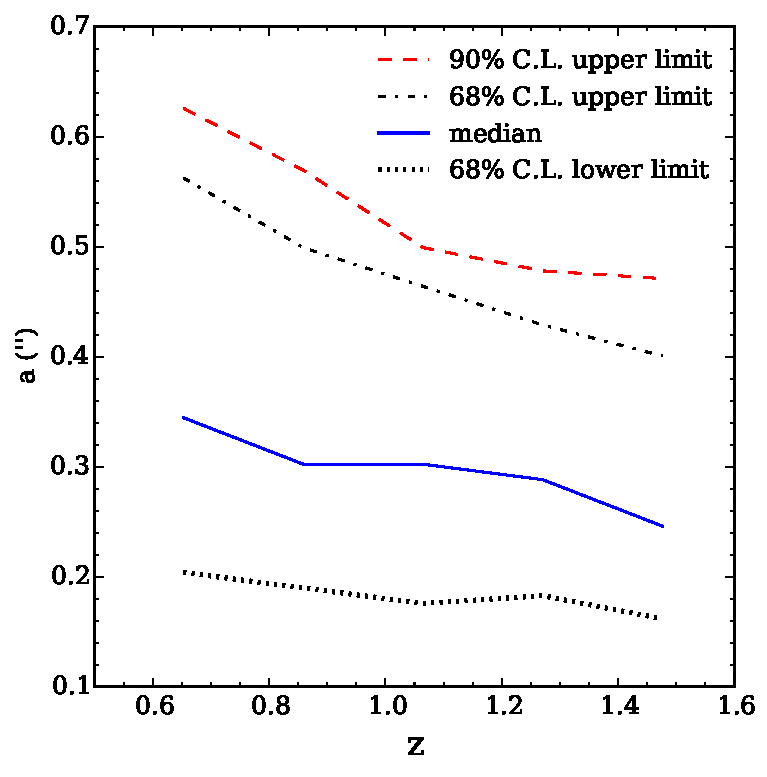
\includegraphics[width = 3.5in]{Plots/size_zbin.pdf}
\label{fig:size_zbin}
\caption{The 90\% upper limit of the semi-major axis
continuum size of H$\alpha$ galaxies with H$\alpha$ line flux $>10^{-16}
\mathrm{erg/s/cm}^2$, $0.55 < z < 1.85$), based on 1773 galaxies from WISP (WISP
team, private communication).} \end{figure}

\paragraph{HLSS 5} Relative position measurement uncertainties shall be less than $3.4''$ over the entire survey area.

 We need to measure galaxy positions to better than $\sim0.1 \mathrm{Mpc}/h$ (which corresponds to $3.4''$, assuming that 105 $\mathrm{Mpc/h}$ subtends 1 degree), in order to measure galaxy clustering accurately. This should be met easily if HLIS 26 is met, which makes systematic errors in the astrometry negligible. Given the pixel scale of $0.11''$, this requirement is automatically met within each field, and is tied to the precision of astrometry across different fields.

\paragraph{HLSS 6} The survey completeness shall be 50\% (TBC), and the redshift purity
 shall be 90\% (i.e., the outlier fraction is less than 10\%). Completeness is
 defined as the fraction of H$\alpha$ ELGs with measured redshifts flagged as reliable, and purity is defined as the fraction of measured redshifts flagged as reliable that are actually within 2$\sigma$ of the true redshifts.

 A requirement on completeness and purity is needed to translate the H$\alpha$ ELG
 number counts predicted by the H$\alpha$ LF to the galaxy number density that can be used to measure BAO/RSD by WFIRST GRS.  The completeness of 50\% and redshift
 purity of 90\% are put in as crude estimates based on extrapolations from
 Euclid.  Since WFIRST has a higher spatial and spectral resolution compared to
 Euclid, and more rolls (4 versus 3) per field, we expect a higher completeness
 and purity for WFIRST.  The actual requirements will need to be validated by
 grism simulations, since these are determined by what are feasible given the
 instrumentation and the true universe.  The requirement on the knowledge on the
 contamination fraction is set by HLSS 4.


 \subsubsection{Implementation Requirements (Level 2b)} In this section, we present the implementation requirements as delivered to the Project Office.

\paragraph{HLSS 7} The observatory shall provide a slitless spectroscopy mode, with a spectral dispersion no larger than 10.85 $\AA$/pix.

 Gratings tend to give constant dispersion in linear space, rather than R-space.
 The above dispersion would give point-source spectral resolution
 $R=\lambda/\Delta\lambda$ in the
 range $550 <R < 800$, for a 2-pixel resolution element.

 The grism resolution requirement is set by requiring the redshift precision to
 be 0.1\% (set by BAO/RSD science), thus is not sensitive to which ELGs (H$\alpha$
 vs [OIII]) we use as tracers. Going to lower spectral resolution would degrade
 the redshift precision and put BAO/RSD science goals at risk. The number density
 of [OIII] ELGs may be significantly higher than previously assumed; this gives
 some margin in the spectral resolution requirement due to the smaller sizes and
 less line blending of [OIII] ELGs.

 Given the margin from a likely higher [OIII] ELG number density than previously
 assumed, we have removed the requirement on resolving H$\alpha$ and NII for all
 galaxies of radius $0.3''$, and 90\% of galaxies of radius $0.54''$, which would drive
 the grism resolution higher. The blending of H$\alpha$ (6563$\AA$) and NII (6584$\AA$) leads to
 a metallicity-dependent shift in line centroid for larger sources
 this would lead to a systematic bias in the measured redshifts, which can
 propagate into the BAO/RSD measurements. Having a higher grism resolution would
 alleviate this problem, at the cost of a reduction in survey depth, and more
 overlapping of spectra for galaxies. This is a trade study that we will carry out
 as the required grism simulations become available.

 \paragraph{HLSS 8} Spectra shall achieve $S/N \geq 5$ for $r_\mathrm{eff} = 300
 \mathrm{mas}$ for an emission line flux $~ 1.0\times10^{-16}\ \mathrm{erg/cm}^2\mathrm{/s}$, from a source at 1.8 $\mu$m.

 This sensitivity is sufficient to meet the comoving space density requirement
 HLSS 2 with some margin given best estimates of the H$\alpha$ luminosity function
 \citep{Pozzetti:2016} at these redshifts. The use of a $\mathrm{S/N} \geq 5$ threshold for an arbitrary spectrum pre-spectral-decontamination gives margin for detection of sources whose spectra overlap others, or for loss of some exposures to cosmic ray hits or other artifacts, as $\mathrm{S/N} \geq 5$ post-decontamination is expected to be
 sufficient for meeting the redshift accuracy requirement HLSS 4, and the
 post-decontamination S/N should be significantly higher than the
 pre-decontamination S/N for a given spectrum. Current calculations of
 observatory performance indicate that the sensitivity specified here is achieved
 in a total exposure time of  $\sim1200$ seconds per field.

 The median continuum size (semi-major axis) of H$\alpha$ ELGs is $0.3''$ (see Figure \ref{fig:size_zbin}).
 This sensitivity requirement is phrased in parallel with the sensitivity requirement
 of the WL survey. This depth is a factor of two to three deeper than the Euclid
 GRS. The depth is sufficient to give the required galaxy number density in HLSS 2.

\paragraph{HLSS 9} The uncertainty of the wavelength measurement $\lambda$ shall satisfy $\Delta\lambda/\lambda \leq 0.001$.

 Although this is redundant since it is essentially the same as HLSS 4, it is
 necessary to keep it since it flows HLSS 4 into a dataset requirement.

\paragraph{HLSS 10} The spectroscopic bandpass shall satify $\lambda_\mathrm{max} \geq 1.9\ \mathrm{\mu m}$, and $\lambda_\mathrm{max}/\lambda_\mathrm{min} < 1.82$.

 We need $\lambda_\mathrm{max} > 1.9\ \mathrm{ \mu m}$ for redshift reach, in order to be complementary to Euclid and ground-based surveys.  Furthermore, we need $\lambda_\mathrm{max}/\lambda_\mathrm{min} < 1.82$ for line identification using multiple lines: to ensure that we cannot have [OII] (373nm) falling off the blue end of our coverage while H$\alpha$ (656.28nm) falls off the red end. We have
 assumed that the actual bandpass extends 1.5\% from either end, since it is
 problematic to use emission lines that fall within 1.5\% of the bandpass edges.

\paragraph{HLSS 11} 50\% of the energy (excluding diffraction spikes and non-1st order light) shall be enclosed in a circle of radius $<0.21^{\prime\prime}$ over 95\% of the field.

 This limit of $0.21^{\prime\prime}$ is required by source separation in the input
 catalog for spectral extraction, and is enabled by the addition of the phase
 mask corrector, and leaves some margin on the wavefront error.

\paragraph{HLSS 12} The filter used to define the bandpass of the grism shall have cutoff transition widths $\sigma < 1\%$ (0.7\% goal) after including the effects of broadening
 by the range of incident ray angles at each position in the FoV, where $\sigma$ is
 defined by $\sigma= (\lambda(T=0.90)- \lambda(T=0.10))/\lambda(T=0.50)$. $T$ is the transmission of the
 grism bandpass.

 This is based on the grism guiding considerations; the assessment of grism
 guiding (and its positive outcome) assumed $\sigma < 1\%$.

 \subsubsection{Implementation (Operations Concept) Requirements} We present here the implementation requirements related to the operation concept. We note that Co-I Hirata is the co-lead for the WFIRST Operations Working Group. We did not update Requirements HLSS 13-15, but include them here for completeness.

\paragraph{HLSS 13} Exposures of each field shall be obtained at a minimum of 3 dispersion directions, with two being nearly opposed.

\paragraph{HLSS 14} The observatory shall be able to place the WFC at a commanded
 orientation with an accuracy of $0.64^{\prime\prime}$ ($3\sigma$) in pitch and yaw, and $87^{\prime\prime}$ ($3\sigma$) in
 roll (TBR these were arbitrary values that give a net $3\sigma$ position uncertainty
 of 10 pixels. For the HLSS, the primary driver is that the position uncertainty
 is small with respect to chip gaps, which gives larger uncertainties than
 specified above. The smaller values quoted here are consistent with efficient
 target acquisitions, which would flow down from an observing efficiency spec.)

\paragraph{HLSS 15} The observatory pointing jitter and drift shall not exceed 100 mas in the spectral direction on the WFC focal plane (goal of 60 mas) and 50 mas in the cross- dispersion direction (TBR).

\paragraph{HLSS 16} Imaging observations shall be obtained of the fields in the HLSS that reach JAB=24.0, HAB=23.5, and F184AB=23.1 for an $r_\mathrm{eff}=0.3^{\prime\prime}$
 source at 10$\sigma$ to achieve a reference image position, in 3 filters.

 Provided the HLSS covers area already observed in the HLIS, this
 requirement will be met automatically.  This requirement applies to any HLSS
 fields that are counted toward the minimum survey area requirement but are not
 covered by the HLIS.  Imaging in at least three filters is required to build a
 minimal spectral template for grism spectral decontamination.

\paragraph{HLSS 17} There shall be 40 observations of two deep fields, each 11 deg$^2$ in area, sufficient to characterize the completeness and purity of the overall galaxy redshift sample. The 40 observations repeat the HLSS observing sequence of 4 exposures 10 times, with each deep field observation having the same exposure time as a wide field observation of the HLSS. The dispersion directions of the 40 observations should be roughly evenly distributed between 0 and 360 degrees.

To calibrate the HLS GRS, we need a spectroscopic subsample, with the same selection criteria as that of the HLS GRS, containing more than 160,000 galaxies  that have a redshift purity $>99\%$. We need 160,000 galaxies to know the redshift purity to 1\% (which requires 10,000 objects, assuming noise of $1/\sqrt{2N}$ from Poisson statistics) in at least four categories (low z, high z, faint, luminous).

Based on the estimated galaxy number density of $>7273$ per deg$^2$ at the flux limit for the GRS, $10^{-16} \mathrm{erg} \, \mathrm{s}^{-1}\mathrm{cm}^{-2}$, we need a total area for the deep fields of 160,000/7273=22 deg$^2$.  These can be split into two subfields of 11 deg$^2$ each.  Smaller subfields prevent the testing of galaxy clustering statistics in each subfield. Each deep field should be part of the HLS footprint, so they are representative of the GRS as a whole.

 The visits to the deep field should consist of 10 sets of HLS-GRS-like visits,
 matching the integration time, dither pattern, and observational time-sequence
 of the HLS-GRS strategy, with each set of HLS-GRS-like visits covering the same
 areas of 22 deg$^2$. Assuming a completeness of 50\% and uncorrelated sets, the
 completeness after 10 sets of visits is (1-0.5)10=0.001, leading to a 99.9\%
 complete sample for calibrating the GRS. Since each set of observation consists
 of 4 roll angles, the total number of deep field observations is 40. The
 dispersion directions of the 40 visits should be roughly evenly distributed
 between 0 and 360 degrees, in order to map out possible sources of systematic
 errors due to inhomogeneity.

\paragraph{HLSS 18} The observing efficiency of the HLSS, defined as the total science exposure time divided by the total time allocated to the survey, shall be TBD\%.

 The total time includes slew, settle, target acquisition, and
 calibration observations that are specific to the HLSS, including the
 extra-depth observations of the deep fields described in HLSS 17.  This minimum
 observing efficiency, together with a 0.67 year total allocation of observing
 time, allows science exposures of 1600 deg$^2$ (TBC) with the exposure time
 indicated in the comment to HLSS 8; this provides a 7\% (TBC) margin over the
 1500 deg$^2$ requirement (HLSS 1) to allow for data that may be unusable because of instrumental artifacts, bright sky objects, etc. This is a high level
 requirement that will need to be revisited as the mission implementation details
 become more solid; it should be set such that the core science goals for the GRS
 are achieved without putting mission success at risk.

\subsubsection{Calibration Requirements} In this section, we present the calibration requirements as delivered to the Project Office.

\paragraph{HLSS 19} The relative spectrophotometric flux calibration shall be known to 2 percent relative accuracy (with the goal of 1\%), in order to understand the effective sensitivity limit for each redshift bin for each area surveyed.

 The requirement here is only on the {\it relative} spectrophotometry, which impacts the selection function of galaxies. Absolute line flux calibration will only change the overall number of objects and the dN/dz, but will not introduce
 density variations.  Large scale structure measurements require precise
 knowledge of the selection function of galaxies. Although the overall redshift
 distribution may be determined by averaging over the entire survey, fluctuations
 in the selection function can easily contaminate the underlying cosmological
 density fluctuations.

 The spectroscopic sample for the GRS is expected to be defined by a line flux
 limit of 10$^{-16}\,$erg$\,$s$^{-1}$cm$^{-2}$. Spatial errors in the spectrophotometric calibration
 will introduce artificial spatial fluctuations in the number density of
 galaxies, which could contaminate the cosmological signal.

 We start by setting a requirement on the spatial uniformity of the mean number
 density as a function of physical scale. We require that the non-cosmological
 fluctuations in the mean number density (or the selection function of the
 survey) be $< 1\%$ (sqrt variance) when averaged over spatial scales between 10
 Mpc/$h$ to 200 Mpc/$h$. At small scales, this is $\sim$ two orders of magnitude smaller
 than the cosmological signal, while at the $\sim$ BAO scale of 100 Mpc/$h$, this
 is $\sim$ one
 order of magnitude smaller than the cosmological signal.  These fluctuations
 equal the cosmological signal at $\sim400 \mathrm{Mpc}/h$.  These physical scales correspond
 to $\sim0.5$ degrees to 6 degrees at a redshift of 1.5.

 We convert the above requirement to a requirement on the spectrophotometric
 calibration accuracy, assuming the Model I luminosity function of \citet{Pozzetti:2016}. At the flux limit of WFIRST, this yields a requirement of 1\% relative spectrophotometric calibration, averaged over angular scales of 0.5 degrees to 6 degrees.

 This is a very stringent requirement. We have relaxed this requirement from 1\%
 to 2\% to add margin for mission success, assuming that we will achieve 1\%
 relative spectrophotometric flux calibration in post-processing by projecting
 out problematic modes in the analysis.

 We plan to make this requirement more precise, in the form of "The relative
 spectrophotometric flux shall be known to 2\% relative accuracy in TBD (probably
 the spectral resolution) wavelength bins with a goal of 1\% on scales larger
 than TBD (per pointing, 0.3 deg) and TBD\% on scales smaller than 0.3 deg.
 We are working on deriving and justifying these numbers.
 Co-I's Capak, Hirata, and Padmanabhan are members of the WFIRST Calibration Working Group, working on a detailed calibration strategy for WFIRST.


\paragraph{HLSS 20} The uncertainty in the wavelength calibration shall not introduce biases in the wavelength measurement by amounts greater than
 $\Delta\lambda/\lambda = 10^{-4}$ on any
 angular scales exceeding 0.064 degrees within a field, and
 $\Delta\lambda/\lambda = 2\times10^{-5}$ from
 field to field.

 Variations in the wavelength calibration within a field, and from field to field
 on large scales, wash out the clustering signal by de-correlating the projected
 component of the clustering signal on those angular scales.

 Within a field, the acceptable level of wavelength error is
 $\Delta\lambda/\lambda \sim 10^{-4}$, which
 is 10\% of the errors on individual redshift measurements (0.001), to avoid
 increasing the overall redshift error by a significant factor. The angular scale
 is set by the optimal smoothing scale for BAO reconstruction, $\sim 5 \,
 \mathrm{Mpc}/h$. At $z=3$, this subtends 0.064 degrees for a flat universe with
 $\Omega_\mathrm{m}=0.3$ and a cosmological constant.

 For field to field, the acceptable level of wavelength error is $2\times10^{-5}$, which comes from comparing two adjacent fields.  Since we expect $\sim 104$ galaxies per deg$^2$, we have $\sim 2810$ galaxies per FOV of 0.281 deg$^2$.  If the galaxies have a redshift error of $10^{-3}$ each, then one can measure systematic offsets between fields (statistically) at the $10^{-3}/\sqrt{2810}$ level, which is $1.9\times10^{-5}$. At that level the power from the systematics is sub-dominant to the power from the redshift error.

 \subsubsection{Requirements on Science Data Products:} In this section, we present the GRS requirements on science data products. We are in the process of studying HLSS 21-25. These depend on the structure and responsibilities of the SOCs and the SITs. Co-Is Teplitz and Capak have extensive experience in data processing for space missions, and have provided detailed comments on these requirements to the WFIRST Project Office.

\paragraph{HLSS 21} The raw data for each grism exposure shall be available through the
 archive, with each dataset including identifying information such as time of
 exposure, observatory pointing orientation, a unique dataset identifier, and any
 engineering information needed for subsequent processing. Each detector readout
 for a given exposure shall be included in the dataset.

\paragraph{HLSS 22} Calibrated data for each grism exposure shall be available through the archive. Each detector readout shall be calibrated at the appropriate level, and the individual calibrated readouts will be combined to produce a net spectral image. These datasets shall include information on the effective PSF as a
 function of position and incorporate any World Coordinate System information
 needed for subsequent stages of processing. As sources are not yet identified,
 association of a pixel with a source position and wavelength is not yet
 possible.

\paragraph{HLSS 23} Source catalogs of the same field derived from WFC imaging data shall be combined with observatory pointing information for each grism exposure to produce a segmentation map that associates each catalog source with a range of spectral image pixels. The spectral images of bright stars in each detector shall be used to refine the astrometric solution.  These segmentation maps shall be used to extract 1D spectra for each source, and to flag pixels that may contain flux from multiple sources. The extracted spectra shall include
 information on the effective exposure time for each pixel, effective PSF as a
 function of position, data quality flags, and any other information needed to
 interpret the data.

\paragraph{HLSS 24} Extracted spectra of each source from multiple roll angles shall be
 combined to produce a single net spectrum of each source. For sources that are
 spatially resolved, the result shall be provided as a data cube of position and
 wavelength. The spectra obtained at nearly opposing roll angles shall be used to
 account for possible offsets of the emitting region from the center of the
 broad-band image. The data from all roll angles shall be used, to the extent
 possible, to resolve ambiguities in the proper source to associate with pixels
 illuminated by overlapping spectra. These net spectra shall include information
 on the effective exposure time for each pixel, statistical and systematic
 uncertainties in the measured fluxes and wavelengths, effective PSF as a
 function of position, data quality flags, and any other information needed to
 interpret the data.

\paragraph{HLSS 25} The data processing system shall have the capability of inserting fake sources into the spectral image data and re-executing the generation of
 high-level science products. These tests are essential for verifying the proper
 operation of the tools that generate high level science products and for
 understanding the sensitivity of the survey and systematic effects that may be
 present in the survey sample.

\paragraph{HLSS 26} The data processing system shall provide sufficient knowledge of the 3D selection function so that the artificial correlations due to inaccuracies in the 3D selection function are less than 10\% of the statistical error bars on
 scales smaller than 2 degrees, and less than 20\% on larger angular scales.

 This requirement is only meaningful in terms of the contribution to the total
 error budget by the uncertainties in the 3D selection function. The BAO scale is
 less than 2 degrees in the redshift range for the HLSS.

 To convert the positions of observed galaxies in the large-scale structure
 into clustering measurements (correlation function, power spectrum, higher order
 statistics) we need to know how the "average" number density of objects (in the
 absence of clustering) changes in the observed volume. The mean number density
 will vary significantly both in redshift and with angular position due to
 effects of target selection, data reduction and observing conditions. Previous
 surveys were able to separate the selection function in two independent parts:
 the radial selection function and the angular selection function. It is likely
 that the WFIRST selection function will not be separable in this way, i.e.
 different parts of the sky will have different radial profiles. For now we will
 assume that this type of separation is possible. This assumption is reasonable
 for preliminary investigation since most effects are either mostly radial (e.g.
 target selection, data reduction) or angular (e.g. imaging quality, galactic
 extinction).

 The knowledge about 3D selection function is usually encoded into sets of random
 catalogues. When computing clustering statistics, the random catalogues remove
 the systematic effects of varying mean number density (due to target selection,
 data reduction or observing conditions). If the 3D selection function is not
 correct, the effects will not be completely removed and will generate spurious
 correlations that can bias the true cosmological signal. The angular mask of the
 WFIRST data will vary pixel to pixel on the infrared detector. The full
 description of the angular mask may turn out to be computationally intractable.
 For the core science goals we require the description of the mask to be correct
 with an angular resolution of approximately 3 arcmin. This corresponds to a
 spatial resolution of $3 \,h^{-1} \mathrm{Mpc}$ at $z=1.5$. This is driven by the fact that we
 need to be  able to resolve the BAO peak. In principle, our requirements on the
 knowledge of the 3D selection function are driven by the main requirement that
 the spurious correlations should be no more than TBD per cent of statistical
 errors between the scales of 10 and 150 h-­?1Mpc in clustering signals (either
 in correlation function multipoles or power-­?spectrum). For the galaxy sample
 expected from WFIRST, this corresponds to TBD per cent uncertainty in the
 knowledge of the radial distribution and the angular mask.

 To further quantify the effect of systematics offset in the angular mask on
 clustering measurements we have performed tests on mock catalogues representing
 BOSS CMASS sample. This is justified by the fact that the BAO and growth rate
 measurements from WFIRST GRS in redshift bins of $z\sim0.1$ are expected to be
 roughly equal to the CMASS constraints with $z\sim0.2$.

 The mock surveys are generated from N-body simulations, with a median redshift
 of 0.6, with galaxies of halo mass range about $7\times10^{13}\,M_\odot$. The mock
 surveys have proper BOSS 3D selection function (which we take as truth here).
 Now we distort the selection function in the following scenarios:


\begin{figure}
 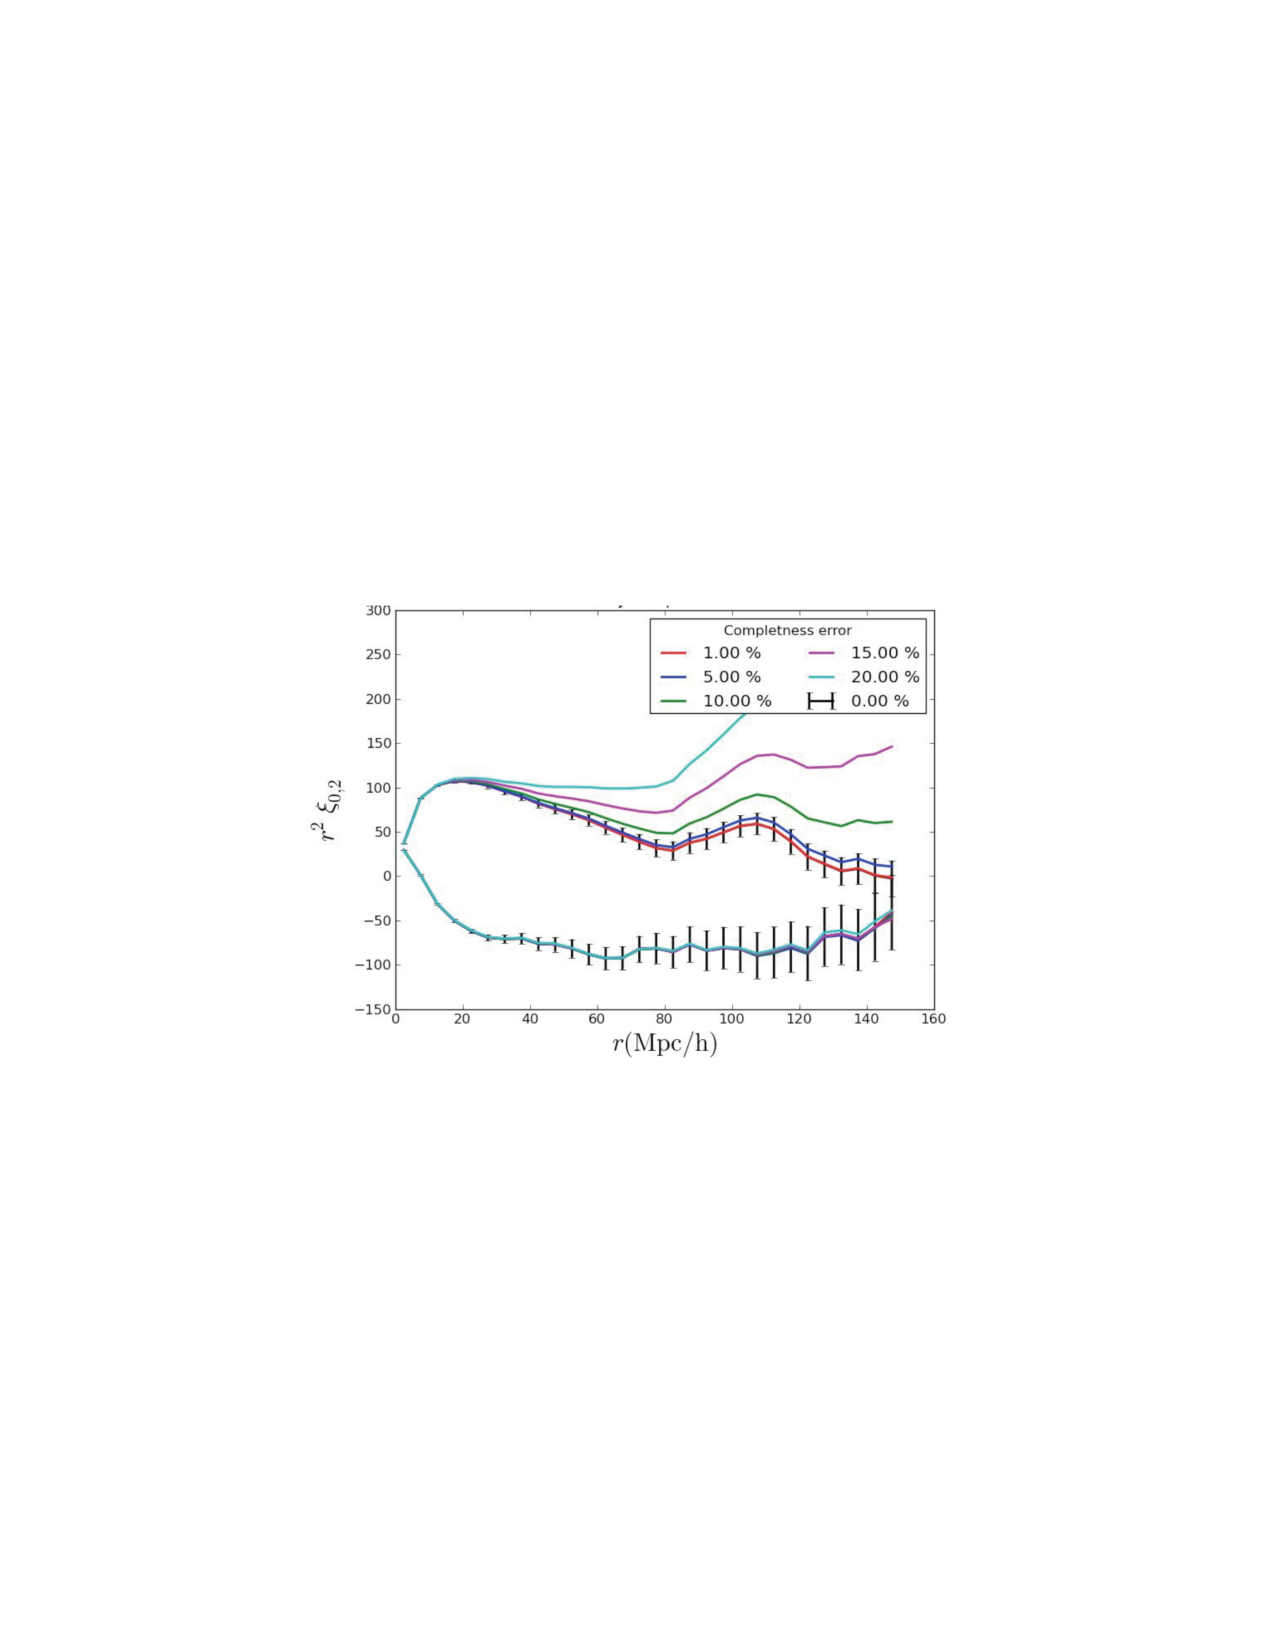
\includegraphics[width =0.75\textwidth]{Plots/GRS_req_1July2016_v3_P6fig.pdf}
 \label{fig:selection_function}
 \caption{The monopole (upper curves) and quadrupole (lower curves) of a single mock survey and how they respond to various completeness errors in the scenario described in scenario. We can see from the level of two point correlation function, even a 5\% error on the completeness can change the monopole   and quadrupole significantly that we expect RSD to be affected, while BAO is not significantly affected, as this mostly changes the amplitude of the correlation function.}
  \end{figure}

\begin{enumerate}
\item The survey region is divided into two equal area along RA and one area
 has true completeness whereas the other one has $1-x$ completeness where x is a
 given completeness error (as shown in the legend of Figure~\ref{fig:selection_function}).
 We show in Figure \ref{fig:selection_function} the resulting monopole and quadrupole with varying completeness error. This
 is an interesting limiting case as surveys can sometimes be affected by large
 scale systematics generated by either calibration of two parts of the sky, or
 due to large scale effects caused by the galactic foregrounds.
\item The true survey completeness is multiplied with a gaussian function. The
 gaussian function has mean 0 and variance as the denoted completeness error. We
 then fold both positive and negative side of the Gaussian to the negative side
 and hence allow the completeness to be only smaller than its true value. We vary
 the scale at which we change the 3D selection function, starting with 1 degree
 to 4 degrees (4 deg. is approximately the BAO scale at this redshift).
 \end{enumerate}
 %In particular, we will show the resulting monopole and quadrupole for 2 degrees and
 %4 degrees in Figure 3 and Figure 4 respectively. These are two interesting
 %limiting cases since they correspond to the extreme situation when the 3D
 %selection function are changed at scales most relevant to linear RSD modeling
 %and BAO analysis.

 From the preliminary analysis shown here, we expect that we will need to
 accurately model the 3D completeness function down to a few \% level.  At 5\%
 the effects can already be very detrimental to our large scale structure
 analyses using BAO and RSD. Scaling from these, we arrive at the requirement
 that artificial correlations due to inaccuracies in the 3D selection function
 are less than 10\% of the statistical error bars on scales smaller than 2
 degrees, and less than 20\% on larger angular scales.

 \subsubsection{Requirement on Cosmological Volume Simulations:} We now present a new category of requirements for a space mission. These are not needed
 for mission success (data acquisition by the spacecraft), but only for meeting the
 high level science requirements (level 1). We summarize these as follows:

 \begin{enumerate}
 \item a few accurate mocks with galaxies included using semi-analytical
 galaxy formation model, to verify and validate WFIRST GRS pipeline;
 \item $\sim 100$ mocks with high mass resolution of 109 solar masses, to inform theoretical modeling of the data;
 \item $\sim 10,000$ mocks with low resolution, to derive the covariance matrices for the WFIRST data.
 \end{enumerate}

 To quantify the requirement on cosmological volume simulations, we consider only
 the case for galaxy clustering science (which includes BAO and RSD) for now for
 simplicity. For WFIRST, simulations are required for the following three
 objectives:
\begin{enumerate}
\item establishing the basic correctness of the pipeline;
\item informing the theoretical modeling of small scale clustering as a function of
 tracer properties;
 \item calculating the covariance matrix for each GRS probe and
 across many probes.
 \end{enumerate}

 In order to establish the basic correctness of the WFIRST pipelines and
 predictions, sophisticated synthetic mock galaxy catalogs are essential.
 These catalogs, which must realistically emulate WFIRST both in sky area and
 depth, are typically constructed by running large gravity-only simulations and
 then ``painting'' realistic galaxies on top.  Populating a simulation with
 galaxies can be done in several ways: (i) empirically, using statistics such as
 the ``halo occupation distribution'', (ii) by placing the normal, baryonic matter
 in the simulation ab initio and explicitly solving the hydro-dynamical
 equations, or (iii) by using a semi-analytical galaxy formation model (SAM),
 whereby the astrophysical processes and formation histories of galaxies are
 described using physically motivated, parameterized equations. The advantage of
 SAMs over alternative methods is their ability to meet the demands from next
 generation cosmological surveys for large (suites of) galaxy mock catalogues
 that are both accurate and can be constructed rapidly. In contrast, full
 hydro-dynamical simulations are far too slow and empirical methods are limited
 by the availability of existing high redshift observations, which are necessary
 for the calibration of these methods. SAMs also require some observations for
 calibration but, once tuned to fit observations at low redshift, they are able
 to make predictions out to high redshift without the need for further
 observational input. Furthermore, empirical methods are often limited in that
 they are calibrated in one or two photometric bands, whilst SAMs are designed to
 model the star formation history of a galaxy and so have the ability to make
 predictions for a wide variety of multi-wavelength data simultaneously. This
 feature of SAMs is vital to ensure that we can examine cross-correlations
 between the spectroscopically-selected dataset for galaxy clustering analysis
 and the photometrically-selected dataset for weak lensing analysis. Besides
 testing the pipeline and making (limited) cosmological forecasts, these galaxy
 mock catalogs would also be a valuable resource for science working groups
 focusing on legacy science (e.g. galaxy evolution, active galactic nuclei). Note
 that,  compared to the large number of approximate mock catalogs necessary for
 covariance estimation, only very few accurate galaxy mocks are required to
 verify and validate the WFIRST pipeline.


 To inform the theoretical modeling of clustering especially at non-linear
 scales as a function of the tracer properties would require a significant number
 of simulations that have relatively realistic modeling of the tracer properties
 at the relevant redshift.  For WFIRST, we can take the current number density of
 emission line galaxies (for H$\alpha$ galaxies only) from our baseline
 calculation and used the \citet{Tinker2008} halo mass function, along with the
 \citet{Giocoli2008} subhalo mass functions to compute the total number of
 halos and subhalos above some mass threshold and then match that to the baseline
 GRS number densities. This maps back to approximately 10$^12$ solar masses from z=1 to z=2. Assuming that we need to have at least 100 particles to resolve halos at
 1012 solar masses, and another factor of 10 particles to resolve properties of
 the halo progenitors, we will need dark matter particle mass resolution of
 approximately 10$^9$ solar masses. The extra factor of 10 is due to the galaxy
 formation model that depends on the properties of the progenitors which is an
 approximation that may change as we understand the galaxy properties better and
 as more observations of the tracers arrive. We expect to require of order 100
 simulations to reduce the shot noise of the correlation function in order to
 compare the theoretical modeling to the simulated correlation function. These
 realistic mock surveys may also require the modeling of non-standard
 cosmological  models, such as extensions to non-zero total neutrino masses, or
 modified gravity models.

 Finally, we will need to calculate the covariance matrices of the main probes of
 clustering, namely BAO and RSD, and the cross-covariances among these probes
 (or across different methods as in recent BOSS analyses). We can approach the
 calculation of the covariance matrices through multiple avenues. One can
 generate (in principle) a large number of approximate mock surveys using
 relatively fast approximate methods (eg., PTHalos, QPM, FastPM, etc), and apply
 the relevant survey properties onto these mock surveys. The small scale modeling
 of the clustering may not be 100\% accurate, but is likely to be adequate for
 the linear RSD modeling and BAO analyses where medium to large scales are most
 important. The number of approximate simulations required can be on the order of
 O(10,000) depending on the number of parameters we will be estimating using
 these covariance matrices, but the time requirement of these approximate mocks
 is relatively modest. One can also envision using more theoretical approaches
 (such as \citet{OConnell:2015src,Padmanabhan2016,Friedrich:2015nga}, which only require a relatively modest number of realistic mock surveys which are required for (b).


\subsection{GRS Light-cone Simulations (D8 and D9)}
%--------------------------------------------------

 \begin{summaryii}
Light-cone cosmological simulations are a critical tool to design the GRS survey design, to develop and to validate analysis tools and theoretical predictions. We developed four complementary simulation approaches to tackle multiple questions relevant to the GRS:
\begin{enumerate}
  \item A lognormal simulation to generate quickly large cosmological volumes;
  \item A fast approach using simple galaxy-halo prescriptions to generate joint GRS and WL simulations;
  \item A realistic emission line galaxies modeling to study the confusion between H$\beta$ and [O III] emitters;
  \item A realistic semi-analytic galaxy evolution model to make robust H$\alpha$ mock catalogs.
 \end{enumerate}
 \end{summaryii}

 In order for WFIRST HLS to reach its  high level science requirements, we have
 proposed to ({\bf D9})  produce simulated light-cone observations to ({\bf D8})
 develop both the methods for modeling and interpretation of cosmological
 measurements from WFIRST.  Most of these data sets will be at the level of
 galaxy redshift and shape catalogs rather than the pixel-level imaging and
 spectroscopy simulations described above. They will incorporate varying degrees
 of complexity regarding galaxy bias, redshift evolution, survey geometry, and
 observational systematics such as incompleteness, shape measurement errors, and
 photometric redshift biases. Many of these artificial data sets will be made
 publicly available, and some will take the form of data challenges, where the
 underlying parameters are initially known only to the creators of the data set.
 Here we report on our first year simulation efforts  in a 4 prong approach,
 ranging from the largest volume to the highest resolution below:

\subsubsection{Lognormal Simulations}

 Samushia and his postdoc have produced a suit of few thousand fast
 ``enhanced log-normal simulations'' for the WFIRST GRS expected samples. While
 these simulations do  not correctly reproduce the small scale structure and
 higher order statistics of the field, they can be used for studying various
 large scale effects and implement light-cone effects. The simulations have so
 far been used to study the effect of splitting the WFIRST footprint into two
 non-contiguous areas. We plan to use these simulations in the future to study
 systematic effects in the measurements (e.g., window effect correction) and to
 validate the BAO/RSD proto-pipeline. These simulations are very well-suited for
 such tasks since their input two-point signal is known exactly.

 \subsubsection{Fast simulations with galaxy positions and shapes}

 Kiessling, and Huff are working with Postdoc Izard to develop a fast
 pipeline to provide galaxy mock catalogues with weak lensing. The goal of our
 initial project is to model effects of various systematics and determine their
 impact on galaxy clustering and weak lensing observables and their covariance
 matrices. The starting point for this project is  300 ICE-COLA fast simulations
 \cite{Tassev:2013pn,Izard:2015dja} generated by Izard during his PhD that
 provide the dark matter density field and halo catalogs (both in the light cone
 geometry). The former is used to compute maps of weak lensing distortions in
 the Born approximation using a technique developed by Izard (Izard et al, 2017;
 in prep). Galaxies are attached to halos using a new pipeline developed for
 this project. This pipeline takes the halo catalogues in the light cone
 geometry generated by the fast simulations and produces galaxy samples with
 broad band luminosities and weak lensing properties. The produced catalogs are
 all sky and span 0 $<$ z $<$ 1.4, with a minimum dark matter halo mass of
 $10^{12}  M_{sun}/h$.

 \subsubsection{Testing the effect of line confusions on BAO using N-body simulations}

  \begin{figure}
   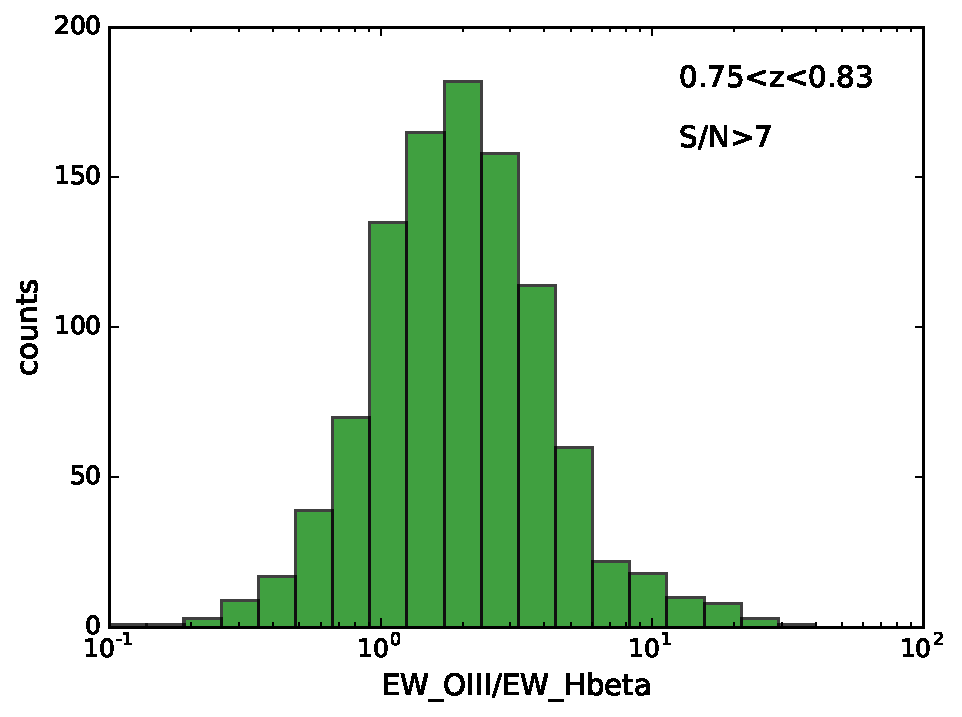
\includegraphics[width = 0.4\textwidth]{Plots/OIII-Hbeta.pdf}
  \label{fig:line-ratios}
   \caption{The line ratios between H$\beta$ and [O III] using the most up to date dataset from SDSS4-eBOSS, which currently has acquired over 10,000 emission line galaxies, but a significant fraction of them have H$\beta$ and/or [O III]. The plot shows $\approx$1000 galaxies from eBOSS sample that has both H$\beta$ and [O III], while each line is detected at least at 7-$\sigma$).}
  \end{figure}

 Ho and Massara concentrates on one particular goal in generating their simulations. Their goal is to investigate the effect of confusion between H$\beta$ and [O III] emitters, in particular in the high level science goal in BAO. In WFIRST,  the primary science targets for the redshift survey will be H$\alpha$ and [O III]. There is a special concern of H$\beta$ vs. [O III] confusion due to their proximity in wavelength (hence the inability of photo-z's to distinguish them reliably). This is particularly true given that an H$\beta$ emitter mis-identified as [O III] will have an inferred radial position different by 8900 km/s (or: 89 $h^{-1} Mpc$ * (1+z)/$\sqrt{\Omega_\Lambda + \Omega_m (1+z)^3}$, which in our range of redshifts is near the BAO scale). We will also get some [O II] emitters -- these might be useful directly for cosmology, or for disentangling other line emitters (see Pullen et al. 2014). Note that at WFIRST resolution 3726 and 2729 are a blend.

 A key challenge in the mocks will be making sure the populations of each line and the correlations among the different line strengths and with environment are sufficiently realistic for the tests we are doing. This has historically proven to be very difficult due to the heterogeneous nature of the observational constraints. Therefore, we have investigated the equivalent width ratio between H$\beta$ and [O III] using the most up to date dataset from SDSS4-eBOSS, which currently has acquired over 10,000 emission line galaxies, but a significant fraction of them have H$\beta$ and/or [O III]. This is so far the only statistical sample that can be used to look at the line ratios (see Figure~\ref{fig:line-ratios}). We also look at the conditional luminosity function between the two line luminosity and found them to be consistent with what was observed in DEEP2 (see Figure~\ref{fig:cond-lum}) with higher statistics. We now proceed to use these line ratios to create the emission line galaxy catalog.

 \begin{figure}
  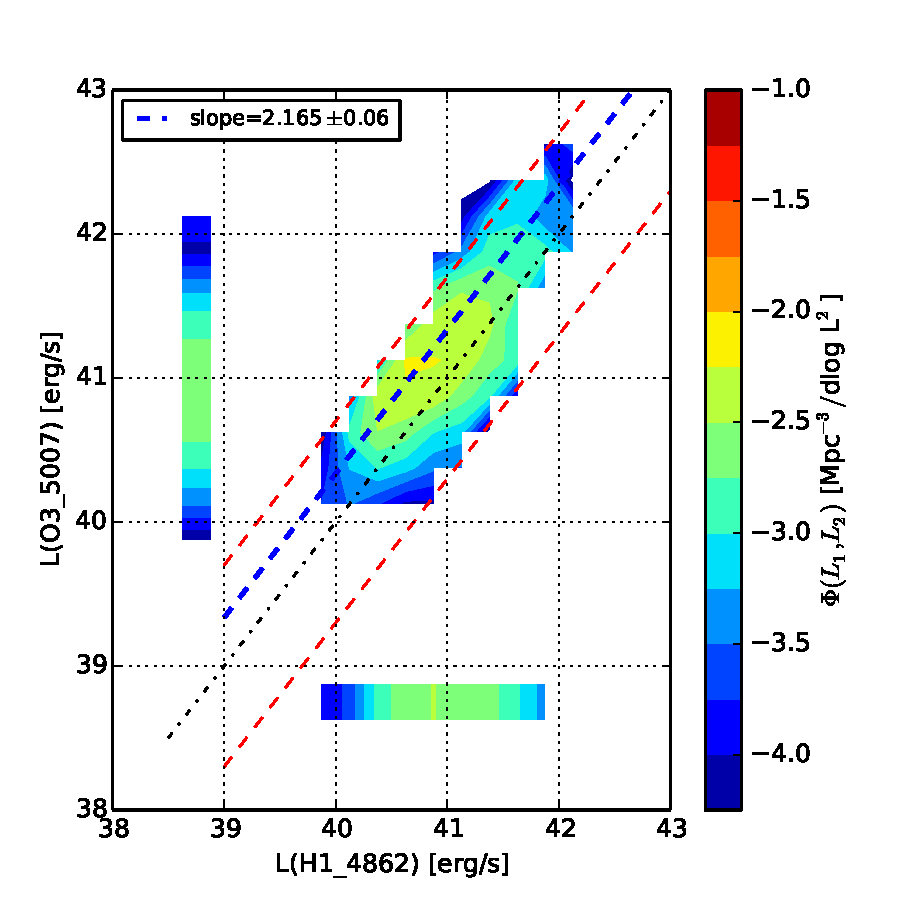
\includegraphics[width = 0.5\textwidth]{Plots/cond_lum.pdf}
 \label{fig:cond-lum}
  \caption{The conditional luminosity function between H$\beta$ and [O III] using the same galaxies as in Figure~\ref{fig:line-ratios}.  The black and red lines are the conditional luminosity function (and 1 sigma) from DEEP2 survey).
 }
 \end{figure}

 We start with dark matter simulations generated by Stanford group (led by Risa
Wechsler, which is part of WFIRST Simulation WG and belongs to the EXPO SIT)
that contain galaxies up to 5-sigma detection limit of grizY = [27.5, 27.0,
26.4, 25.9, 24.0] over 10313 sq. degrees.  Each of the galaxy contain its own
spectral energy distribution which are generated to fit most updated luminosity
function and color evolution measurement. Galaxy magnitudes and shapes are
affected by shear and magnification. We then measured and validated the
correlation function and luminosity function of [O III] selected galaxies (with
WFIRST detection limits) (see Figure~\ref{fig:corr-func}. Next, we plan to apply
the measured line ratios as described in Figure~\ref{fig:line-ratios} to all the
galaxies and reapply the WFIRST detection limits to create a realistic WFIRST
emission line galaxy catalog (with  [O III] as the main galaxy targets), and
assess the effects on BAO peak position due to the possible smearing by
mis-identifying the H$\beta$ as [O III]. In addition to the mocks themselves, it
will be important for us to identify which aspects of the emission lines we
think are close to reality, which are of the right order of magnitude, and which
could be qualitatively different from the real Universe. We envision that we
would continue improving these up to the point where we have the real WFIRST
data.

 In addition, we have also released a code that calculates the interloper
 fraction (Wong, Pullen \& Ho): a Python-based program that applies secondary
 line identification and photometric cuts to mock galaxy surveys, in order to
 simulate interloper identification. We also have a module specifically designed
 to do WFIRST and predict interloper rates for WFIRST \citep{Wong:2016eku}.

 \begin{figure}
 %\includegraphics[width = 3.5in]{corr-func.pdf}
 \label{fig:corr-func}
 \caption{The correlation function of [O III] galaxies with WFIRST detection limit within our 10,000 sq.deg simulations.
 }
 \end{figure}

\subsubsection{H$\alpha$ emitter number density forecasts.} %Simulating Realistic Emission Line Galaxies}

%Wang and Merson have focussed so far on investigating the emission line
%properties of galaxies as predicted by the open-source semi-analytical galaxy
%formation model, \textsc{Galacticus} \citep{Benson:2010kx,Benson2012}). The %first stage of
%this work has been to examine the H$\alpha$ number counts predicted by the model
%and compare the predicted cumulative number density of H$\alpha$ emitters to
%observations from the WISP survey \citep{Colbert:2013ita,Mehta:2015}. By
%adjusting the strength of dust attenuation we are able to obtain %\textsc{Galacticus}
%counts that are in agreement with the WISP observations. I have therefore used
%\textsc{Galacticus} to make predictions for the number density of H$\alpha$ %emitters that will be detected for WFIRST.  Assuming a flux limit of $10^{-16}$ %erg/s/cm$^2$,
%\textsc{Galacticus} predicts WFIRST to observe a number density of 26,000-29,000
%H$\alpha$ emitters per square degree over the redshift range 0.5 $\leq$ z $\leq$
%2. I am now finalizing a paper discussing this work. In addition they have also
%been working on extracting equivalent widths and SEDs for \textsc{Galacticus} %galaxies.
%Code to extract these properties has been included in \textsc{Galacticus}, though these
%features are still be be tested.

% Other WFIRST progress that are not yet a deliverable:
% - We are working on constraining the intrinsic alignment models using filaments constructed from spectroscopic surveys. The idea being that in WFIRST, we can do this for the first time using photometric survey and spectroscopic survey together and mitigating the strongest astrophysical systematic -- intrinsic alignment by modeling it out.  We have measured the intrinsic alignments with LOWZ galaxies and the paper is in prep right now. (Chen, Ho, Mandelbaum, Blazek et al.)

In work led by Merson, Wang, Benson, Kiessling and Rhodes the open source
semi-analytical galaxy formation model, \textsc{Galacticus}
\citep{Benson2010,Benson2012}, was used to predict the H${\rm \alpha}$-emitter number counts and redshift distributions for the
WFIRST GRS. This work is published in \citet{Merson2017}.

A four square degree lightcone catalogue was constructed by processing
the dark matter merger trees of the Millennium Simulation
\cite{Springel05} with the \textsc{Galacticus} model. Emission lines
are modelled in \textsc{Galacticus} by interpolating over a library of
emission line luminosities obtained from the \textsc{Cloudy}
\cite{Ferland13} code and stored as a function of hydrogen (HI),
helium (HeI) and and oxygen (OII) ionising luminosities, as well as
the hydrogen gas density and metallicity of the interstellar medium
(ISM). The emission line luminosities are then processed to
incorporate attenuation due to interstellar dust, which can be
modelled using several different methods. Merson and collaborators
consider three dust methods from \citet{Ferrara99}, \citet{Charlot00} and \citet{Calzetti00}. However, it is worth noting that any user-specified dust method can be used in conjunction with \textsc{Galacticus}.

\begin{figure}
  \centering
  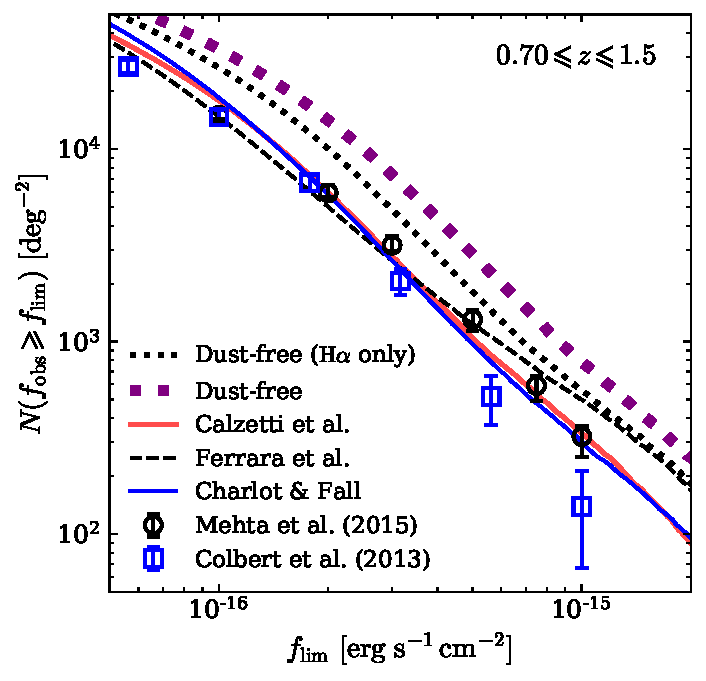
\includegraphics[width=3.5in]{Plots/merson17LightconeHalphaCumulativeCounts.pdf}
  \caption{Predictions for the cumulative H${\rm \alpha}$ flux counts
    for the redshift range $0.7<z<1.5$ from a \textsc{Galacticus}
    lightcone mock catalogue. The various lines show the predictions
    for the pure H${\rm \alpha}$ fluxes and the H${\rm \alpha}$ fluxes
    when blended with NII (H${\rm \alpha}+{\rm NII}$), assuming either
    no dust attenuation or attenuation using one of three methods:
    Ferrara \textit{et al.} (1999) \protect\cite{Ferrara99}, Charlot
    \& Fall (2000) \protect\cite{Charlot00} or Calzetti \textit{et al.} (2000) \protect\cite{Calzetti00}. To be consistent with
    the observed counts from WISP \protect\cite{Colbert13,Mehta2015},
    which are shown by the data points, contamination from NII is
    assumed to contribute 29 per cent to the galaxy luminosity. For
    the Calzetti \textit{et al.} \protect\cite{Calzetti00} method we
    adopt $\tau_{\rm V}\simeq0.83$. For the Charlot \& Fall
    \protect\cite{Charlot00} method we adopt $\hat{\tau}^{\rm ISM}_{\rm V}=0.05$ and $\hat{\tau}^{\rm MC}_{\rm V}=0.04$. When
    applying attenuation due to molecular clouds (MCs) to the Ferrara
    \textit{et al.}  \protect\cite{Ferrara99} method we also assume
    $\hat{\tau}^{\rm MC}_{\rm V}=0.04$.}
  \label{fig:halpha_flux_counts}
\end{figure}

First, the \textsc{Galacticus} predictions for the cumulative counts of H${\rm
\alpha}$-emitting galaxies over the redshift range $0.7\leqslant z\leqslant 1.5$
obtained with each dust method are compared with the latest WISP counts from
\citet{Mehta2015}. The H${\rm \alpha}$ luminosities from \textsc{Galacticus} are
corrected to introduce contamination due to NII by assuming that NII contributes
29 per cent to the observed emission line luminosity. A fixed NII contamination
was chosen to be consistent with the WISP analyses of \citet{Colbert13} and
\citet{Mehta2015}. By adjusting the parameters used by two of these dust models,
the \citet{Charlot00} method and the \citet{Calzetti00} dust law, the authors
are able to obtain predicted cumulative H${\rm \alpha}$ flux counts from
\textsc{Galacticus} that are consistent with the observed counts of \citet{Mehta2015} down to a flux limit of $1\times 10^{-16}{\rm
erg}\,{\rm s}^{-1}{\rm cm}^{-2}$ (see Figure~\ref{fig:halpha_flux_counts}).
Adopting the Ferrara \textit{et al.} \citet{Ferrara99} dust method yields counts
that agree with the observations for flux limits fainter than approximately
$5\times 10^{-16}{\rm erg}\,{\rm s}^{-1}{\rm cm}^{-2}$, but yield an excess in
the number counts for the brightest fluxes. Overall the authors find that down
the expected flux limits of the WFIRST mission, the \textsc{Galacticus} model is
able to predict number densities that are consistent with existing observations
from the WISP survey. Although the lightcone used in this analysis has a small
area on the sky, it is expected that cosmic variance has little effect on the
predicted number counts. Since the lightcone analysis is time-consuming and
expensive in computing resources, the lightcone used in this study was limited
in size to 4 sq deg, in order to provide timely input to WFIRST. However, the
authors plan to build significantly larger lightcones in future work.

After setting the strength of the dust attenuation for each method the
authors then examine whether these chosen attenuation strengths yield
reasonable matches to the observational estimates for the distribution
of optical depth (at the observer-frame H${\rm \alpha}$ wavelength)
and the H${\rm \alpha}$ line luminosity function. For each of the dust
models, \textsc{Galacticus} predicts optical depths that are
consistent within error with the optical depth estimates from WISP
\citep{Dominguez13}, though the \textsc{Galacticus} optical depths do
not show any increase with observed H${\rm \alpha}$ luminosity, as has
been suggested in the literature. The predicted luminosity function
from \textsc{Galacticus} is consistent with the H${\rm \alpha}$
luminosity function from WISP as measured by \citet{Colbert13} over the redshift range $0.9\leqslant z \leqslant 1.5$. Comparison with the luminosity functions from HiZELS \citep{Sobral13} at $z\simeq 0.84$, $z\simeq 1.47$ and $z\simeq 2.23$
shows that with these chosen dust attenuations \textsc{Galacticus} is
able to reproduce the $z\simeq 0.84$ luminosity function, but becomes
progressively a worse fit towards higher redshift, especially at
$z>2$. This suggests that the dust methods may be lacking some
redshift evolution or dependence on other galaxy properties, or that
the \textsc{Galacticus} emission line luminosities are the
incorrect\ strength. Investigating these possibilities requires
rigorous calibration of the \textsc{Galacticus} model, which will be
carried out in future work.

\begin{table*}
\centering
\caption{Predicted cumulative number of H${\rm \alpha}$-emitting
  galaxies per square degree for the WFIRST GRS, assuming a redshift
  range of $0.5\leqslant z\leqslant 2$. The upper half of the table
  shows the counts for NII contaminated fluxes, whilst the lower half
  of the table shows the counts when NII contamination is
  removed. Predicted counts are reported for three dust methods:
  \citet{Calzetti00}, \citet{Charlot00} and \citet{Ferrara99}. For the Ferrara \textit{et al.} method we include attenuation due to molecular clouds (MCs). The
  strength of the attenuation for the various methods are the same as
  in Fig.~\ref{fig:halpha_flux_counts}. Note that the flux limits
  assume contamination by NII, which is set at 29 per cent of the
  total flux, as adopted by \citet{Colbert13}. The efficiency of each survey is
  instrumentation dependent, and has not been included.}
\begin{tabular}{|c|c|c|c|}
\hline
Flux limit&\multicolumn{3}{|c|}{Dust method used with \textsc{Galacticus}}\\
${\rm erg}\,{\rm s}^{-1}{\rm cm}^{-2}$&Calzetti \textit{et al.} (2000) & Charlot \& Fall (2000) & Ferrara \textit{et al.} (1999, inc. MCs)\\
\hline\hline
\multicolumn{4}{|c|}{\textsc{Cumulative counts including NII contamination}}\\
$1\times 10^{-16}$&26344&28958&26730\\
$2\times 10^{-16}$&9169&10439&10571\\
$3\times 10^{-16}$&4675&5378&6013\\
\hline
\multicolumn{4}{|c|}{\textsc{Cumulative counts with NII removed}}\\
$1\times 10^{-16}$&15833&17660&16938\\
$2\times 10^{-16}$&5202&5971&6557\\
$3\times 10^{-16}$&2628&2978&3751\\
\hline
\end{tabular}
\label{tab:cumulativeFluxCounts}
\end{table*}

Finally, the \textsc{Galacticus} lightcone is used to present predictions for
the redshift distribution and the differential and cumulative H${\rm \alpha}$
flux counts for the WFIRST GRS, as well as two surveys mimicking a Euclid-like
selection. These predicted cumulative flux counts to are compared to forecasts
from \citet{Mehta2015} and empirical models originally presented by
\citet{Pozzetti15}. The \textsc{Galacticus} forecasts have counts that are
consistent with those of \citet{Pozzetti15} and about 30 per cent lower than
those of \citet{Mehta2015}. The deficit compared to the Mehta \textit{et al.}
forecasts could be due to Mehta \textit{et al.} using the OIII line to
extrapolate the number of H${\rm \alpha}$ emitters for $z\gtrsim1.6$. For a
WFIRST GRS with redshift range $0.5\leqslant z\leqslant 2$ and flux limit of
$1\times 10^{-16}{\rm erg}\,{\rm s}^{-1}{\rm cm}^{-2}$ \textsc{Galacticus}
predicts a number density between 26,300 and 29,000 galaxies per square degree,
prior to removal of NII contamination, and 29 per cent lower with NII removed.
Note that all the H${\rm \alpha}$-emitter counts discussed in this paper are
expected number counts of target galaxies for spectroscopy, and \emph{not} the
counts of galaxies with redshift measurements. The latter will depend on the
redshift purity and completeness for each survey, which in turn depends on
instrumentation and noise parameters.

\begin{summary}
In this section, we have illustrated that our multiple simulation efforts
complement each other in different ways. LogNormal and Fast simulations with
both positions and shapes,  are useful for pipeline testing and constructing
covariance matrices. The more realistic simulations will test various assumption
and requirements we make for WFIRST HLS. For example, do we need higher
resolution in the grism to disentangle the [O III] and  H$\beta$? Do any of
these line ratios or galaxy properties depend on environment?  Would it lead to an environment dependent BAO smearing if we do not take these into account?  As
we develop more realistic galaxy simulations such as those with \textsc{Galacticus}, we will be able to use the appropriate prescription for
galaxy properties we cannot measure with current observations and make our final
WFIRST simulation as realistic and physically driven as possible. We will examine a variety of other properties of emission line galaxies, including the distribution of OIII luminosities fluxes and the contamination from NII.
This will allow us to have the best tool to develop both the methods for modeling and interpretation of cosmological measurements from WFIRST, and release the most
realistic WFIRST galaxy catalog to the public before WFIRST launch.
\end{summary}

\subsection{Improving our Knowledge of the H$\alpha$ Luminosity Function}
\label{sec:LF}
\begin{summaryii}
Knowing the H$\alpha$ and [OIII] luminosity functions is critical in order to optimize the WFIRST GRS. We are addressing current limitations in our knowledge using a newly available set of HST spectroscopic data within the WISP collaboration.
\end{summaryii}

In order to trace the galaxy distribution through z$\sim$2.7, the future WFIRST
surveys will make use of H$\alpha$ and [OIII] selected emission line galaxies.
These two lines will allow WFIRST to cover the redshift range 1$<$z$<$2
(H$\alpha$) and 2$<$z$<$2.7 ([OIII]) respectively. Therefore, knowing the
expected number of H$\alpha$ galaxies in the survey volume is required and the
study of the H$\alpha$ luminosity function (LF) become fundamental in order to
optimize the planned redshift surveys. However, despite the numerous works on
this topic, given the high uncertainties associated to the H$\alpha$ LF
determination, a sufficiently precise measure is still lacking
(Figure~\ref{fig:img_depths}). Additionally, the samples of emission-line
galaxy are expected to be affected by a complex selection function that depends
on galaxy luminosity, size, line equivalent width and also on contamination from
mis-identified single emission-line galaxies at different depths.

A newly available set of HST spectroscopic data, gathered in the context of the
WFC3 Infrared Spectroscopic Parallel (WISP) survey \citep{Atek:2010},
of which team members Teplitz and Baronchelli are members, has recently become
publicly available. Currently, this survey covers a total area of more than
$\simeq$ 2000 sq. arcmin., with thousands of emission lines from a total
of $\sim$500 randomly distributed HST pointings identified between z=0.3 and
z=1.5. Thousands of emission lines from a total of $\sim$500 randomly
distributed HST pointings have already been identified by the WISP team, between z=0.3 and z=1.5. The spectroscopic capabilities of HST+WFC3 are comparable to those that WFIRST can reach over a 2-order of magnitude wider area. This fact makes the WISP survey a particularly suitable test bench to optimize the future WFIRST surveys.

The accurate constraint of the parameters defining the line LF ($\phi^{*}*, L^{*}, \alpha$) is hindered by their high correlation. Therefore, estimating these parameters requires uniform sampling of both the bright and faint ends of the luminosity distribution. In the next months, in the context of a collaboration involving both WISP and SIT members, Teplitz, Baronchelli and Wang, are planning to obtain the most accurate estimate, to-date, of the H$\alpha$ and [OIII] LFs in the redshift range 0.7-1.6 and 2-2.2 respectively. This result will be achieved by combining deep and shallow data from various HST-WFC3 slitless spectroscopic surveys: WISP (\citet{Atek:2010}, PI: Malkan, M.), the SN followup of the CANDELS survey (SN-CANDELS, PI: Riess, A.), 3D-HST (\citet{VanDokkum:2011,Brammer:2012}, PI: Van Dokkum) and AGHAST (A Grism H-Alpha SpecTroscopic survey in the GOODS-N, PI: B. Weiner).
%In the next months, by combining deep and shallow WISP, CANDELS SN and 3D-HST+AGHAST datasets, Harry Teplitz, Ivano Baronchelli and Yun Wang, in a collaboration between the SIT and the WISP teams, are planning to obtain the most acurate estimate, to-date, of the H$\alpha$ and [OIII] LFs in the redshift range 0.7-1.6 and 2-2.2 respectively.
Since previous studies suggest a substantial brightening of $L^{*}_{H\alpha}$ (Figure~\ref{fig:img_depths}), this study will be performed by dividing the sample in three redshift bins between z=0.7 and z=1.6. Even if split, the combined sample is large enough to allow for an uniform coverage of the $H\alpha$ luminosity range, from few \% of $L^{*}_{H\alpha}$ to many times $L^{*}_{H\alpha}$.

\begin{figure}[!t]
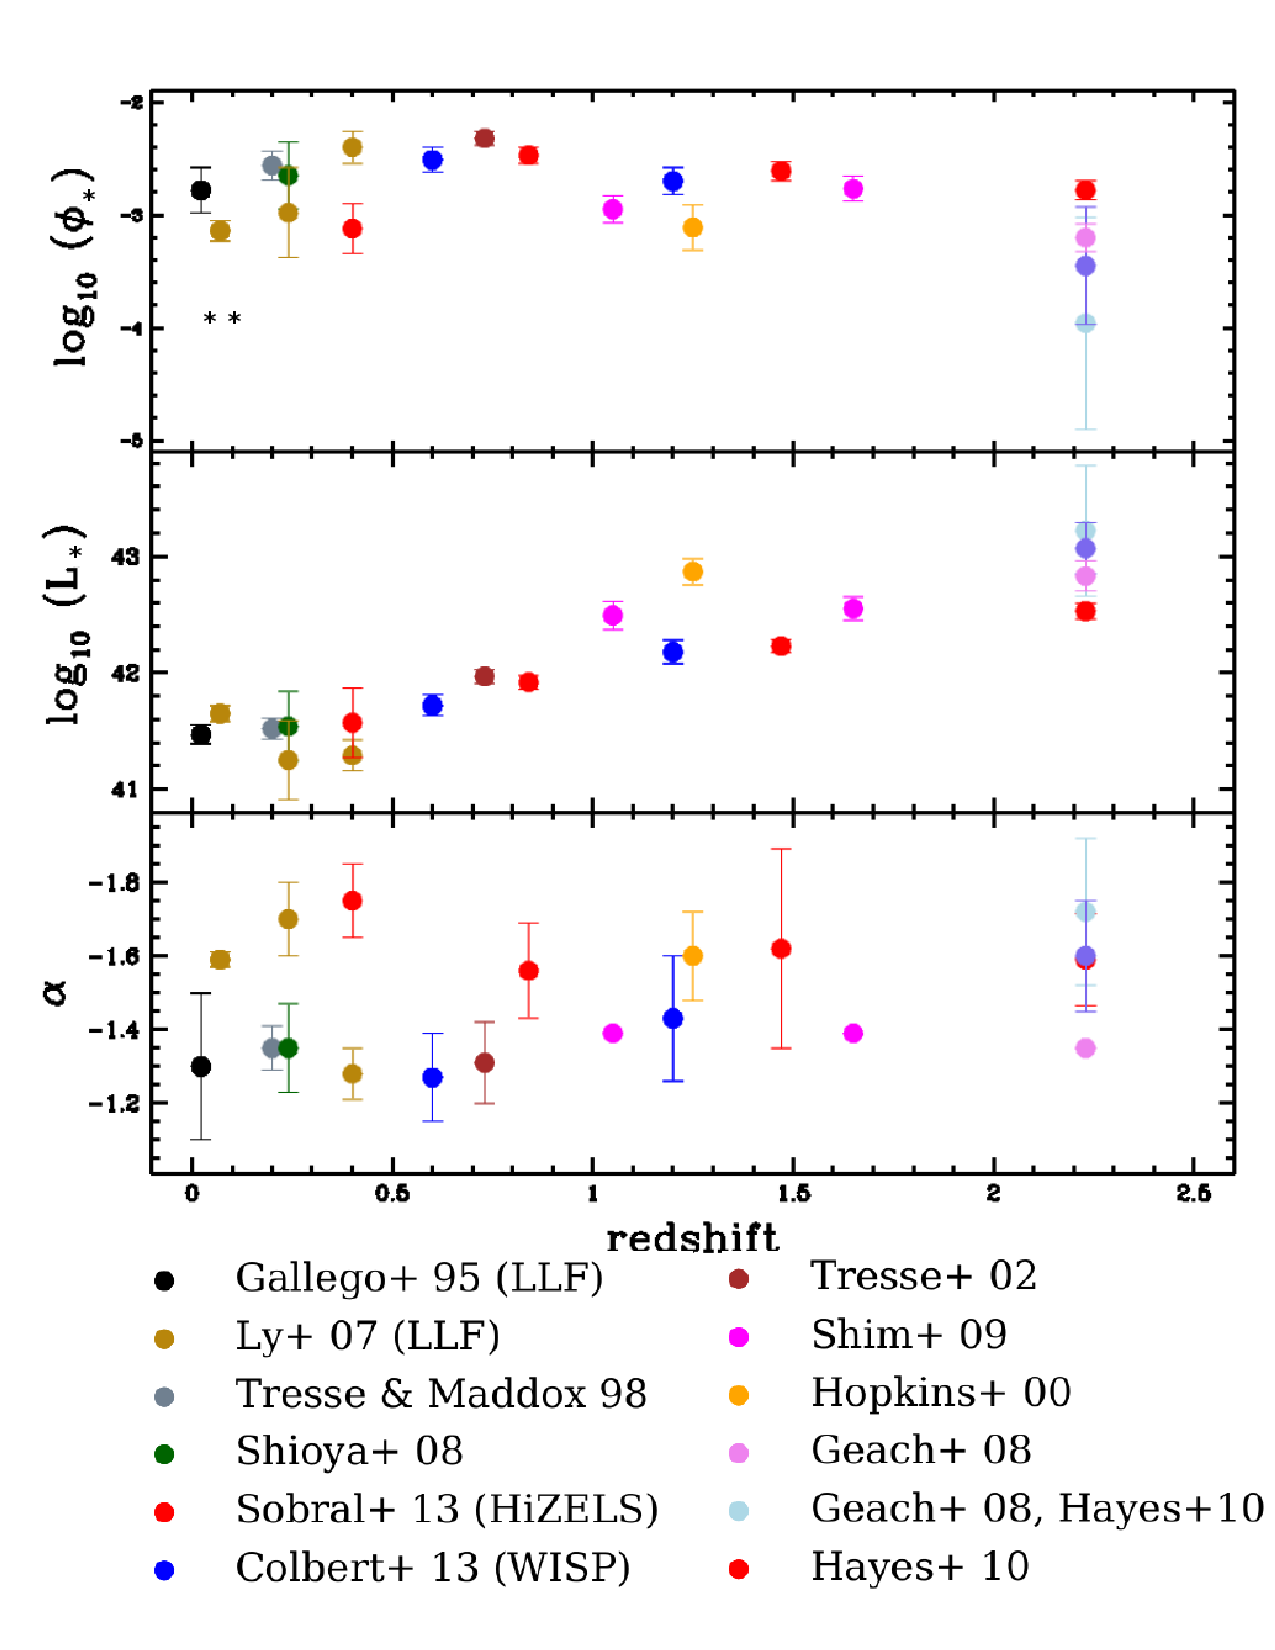
\includegraphics[width=0.5\textwidth]{Plots/HA_LF.pdf}
%\includegraphics[width=7.5cm]{WFIRST_WISP_comparison.eps}
\caption{H$\alpha$ LF as estimated in various surveys. The uncertainties on the different parameters defining the LF are considerable. The aim of this project is to measure the most precise H$\alpha$ and [OIII] luminosity functions to-date, in the redshift range 0.7-1.6 and 2-2.2 respectively.}%{\bf 1B)} Redshift and wavelength coverage for planned WFIRST surveys compared with WISP and Euclid. The shaded regions indicate the full wavelength and redshift ranges of
\label{fig:img_depths}
\end{figure}

Above z=1.6, the H$\alpha$ line is redshifted outside the detectable wavelength
range and since single line emitters are considered H$\alpha$ by default, the
ability to confirm the identification of [OIII] lines is limited to bright lines
with clear shapes. Greatly extending the small dataset used in
\citet{Colbert:2013ita}, the newly released WISP data will allow us to better
constrain the contamination of the H$\alpha$ selected sample, and the loss of
completeness of the [OIII] sample. We will use the multi-wavelength dataset on
3D-HST + AGHAST to identify a combination of colors that could possibly mitigate
this problem.

The identification of the spectral lines and the measure of their fluxes is
fundamental for all the successive part of the LF project here described, but it
can not be completely performed by an automatic algorithm. Thanks to the same
collaboration involving both the SIT and WISP team members, automatic softwares
have already been optimized to i) remove low S/N detections and some of the
contaminating false detections and ii) measure the total line fluxes after their
identification. However, the human interaction is required to visually identify
each detected line (mostly H$\alpha$ and [OIII], but also OII, H$\beta$ and
SII), to perform high quality continuum and line fits, and to remove not
automatically identified contaminants. In the past weeks, the work has been
focused on these tasks. As a result, a large dataset of thousands of objects
with measured line fluxes and corresponding redshift is now available.
% Using the same data, the continuum luminosity, galaxy size and EW distribution functions for line emitters can be constrained.

At the end of the work described in this section, for which more than a semester is still reasonably required, the results will bring to a publication, in one of the major journals, with the co-authorship of Teplitz, Baronchelli and Wang.


 \subsection{Cosmological Forecasting and Data Analysis Algorithms}

 \begin{summaryii}
  We have developed software package to make quick forecasts on basic dark energy parameters from higher order statistics, incluging power spectrum and bispectrum multipoles. This light and agile software package will be the backbone of our GRS proto-pipeline effort.
  \end{summaryii}

 The key dark energy constraints from the WFIRST GRS will result from the BAO and
 RSD measurements from the two-point statistics of the observed galaxy field.
 Similar measurements from the higher order statistics are weaker and currently
 are considered less robust. Cosmological constraints from higher order
 statistics scale very steeply with the number density and since WFIRST GRS will
 provide very dense galaxy samples they may significantly enhance the yield from
 the standard two-point BAO/RSD analysis. We also expect the methods of analyzing
 higher order statistics to become more robust and standardized by the time of
 WFIRST launch. Because of these considerations it would be helpful to have a
 higher order statistics forecasting tool. We have developed software package to
 make forecasts on basic dark energy parameters from higher order statistics.
 The main assumptions are similar to the ones made in the standard
 power-spectrum forecasting tool used for baseline WFIRST predictions. We will
 work on integrating this software with the standard forecasting tool developed
 by our SIT. While the key design decisions will still be based on the
 two-point statistics forecasts, knowing how different choices will effect higher
 order analysis will be very informative.

 The KSU group has assembled a fast and lightweight set of tools for analyzing
 the WFIRST GRS data. Currently this toolset starts from the redshift catalogue
 and the visibility cube and produces the measurements of power spectrum
 multipoles. The multipoles are then analyzed to extract the BAO and RSD signal
 from them. The BAO extraction algorithms replicate the analysis of the final
 BOSS DR12 sample. The RSD analysis is currently simplistic and uses the linear
 model. We will update this toolset by implementing more realistic RSD models.
 The toolset will eventually be linked to the redshift catalogue and visibility
 cube producing software. This software will provide the backbone of our BAO/RSD
 proto-pipeline and will be validated with high fidelity WFIRST simulations.


 \begin{summary}[Future Work on Galaxy Redshift Survey]
 \begin{enumerate}
 \item We will keep refining and solidifying the scientific requirements;
 \item We will pursue our light-cone simulations and release mock catalogs to the community when publishing our results;
 \item We will pursue our effort with image simulation, relying on the light-cone simulation to incorporate realistic galaxy distributions and properties;
 \item We will continue our pseudo-pipeline effort;
 \item \Oli{TO BE CONTINUED}.
 \end{enumerate}
 \end{summary}


%===============================
\section{Cosmological Forecasts}
%===============================
\label{sec:forecast}
\newcommand{\nn}{\nonumber}
\newcommand{\vpi}{\mathbf \pi}
\newcommand{\vecd}{\mathbf d}
\newcommand{\matC}{\mathbf C}
\newcommand{\matQ}{\mathbf Q}

\newcommand{\om}{\Omega_\mr m}
\newcommand{\omb}{\Omega_\mr b}
\newcommand{\sig}{\sigma_8}
\newcommand{\ns}{n_s}
\newcommand{\w}{w_0}
\newcommand{\wa}{w_a}

\renewcommand{\d}{{\rm d}}
\newcommand{\pd}{P_{\delta}}
\newcommand{\pe}{P_\mr E}

\newcommand{\vt}{\vartheta}
\newcommand{\vp}{\varphi}
\newcommand{\eps}{\epsilon}
\newcommand{\abs}[1]{| #1 |}
\newcommand{\mr}{\mathrm}

\renewcommand{\d}{{\rm d}}

\newcommand{\like}{L}
\newcommand{\prob}{P}
\newcommand{\probr}{P_r}
\newcommand{\p}{\mathbf p}
\newcommand{\pco}{\mathbf p_\mr{c}}
\newcommand{\pnu}{\mathbf p_\mr{n}}
\newcommand{\plf}{\mathbf p_\mr{LF}}
\newcommand{\D}{\mathbf D}
\newcommand{\Del}{\mathbf \Delta}
\newcommand{\M}{\mathbf M}
\newcommand{\N}{\mathbf N}
\newcommand{\U}{\mathbf U}


In this section we detail the results of a variety of simulated likelihood analyses that forecast science return and systematics studies of different choices in the WFIRST HLS survey. We first introduce the CosmoLike software framework that was used to generate the forecasts, followed by sections that are dedicated to forecasting the HLSS and HLIS specific observables. We conclude with a summary of the ongoing research to explore WFIRST multi-probe analysis strategies, i.e. to combine all WFIRST observables and their correlated systematics consistently in simulated likelihood analyses. This section also contains an outlook of our ongoing synergy studies to assess synergies of WFIRST and other contemporary surveys, e.g. the ground-based, optical Large Synoptic Survey Telescope (LSST) and future missions studying the Cosmic Microwave Background, e.g. the CMB-Stage4 (CMB-S4) experiment.

\subsection{CosmoLike Introduction}
\label{sec:cosmolike}
CosmoLike has been used in several science efforts, e.g. the combined probes forecasts presented in \citep{Eifler2014}, the analysis of SDSS shear data \citep{Huff2014}, and in efforts to develop new mitigation strategies for baryonic physics \citep{Eifler2015} and galaxy intrinsic alignment \citep{Krause2016}. It is one of two cosmology analysis pipelines within for the ongoing Dark Energy Survey's Year 1 analysis and it has previously been used in the DES science verification data analysis \citep{The DES Collaboration 2016}. Beyond DES,  

\begin{figure*}
  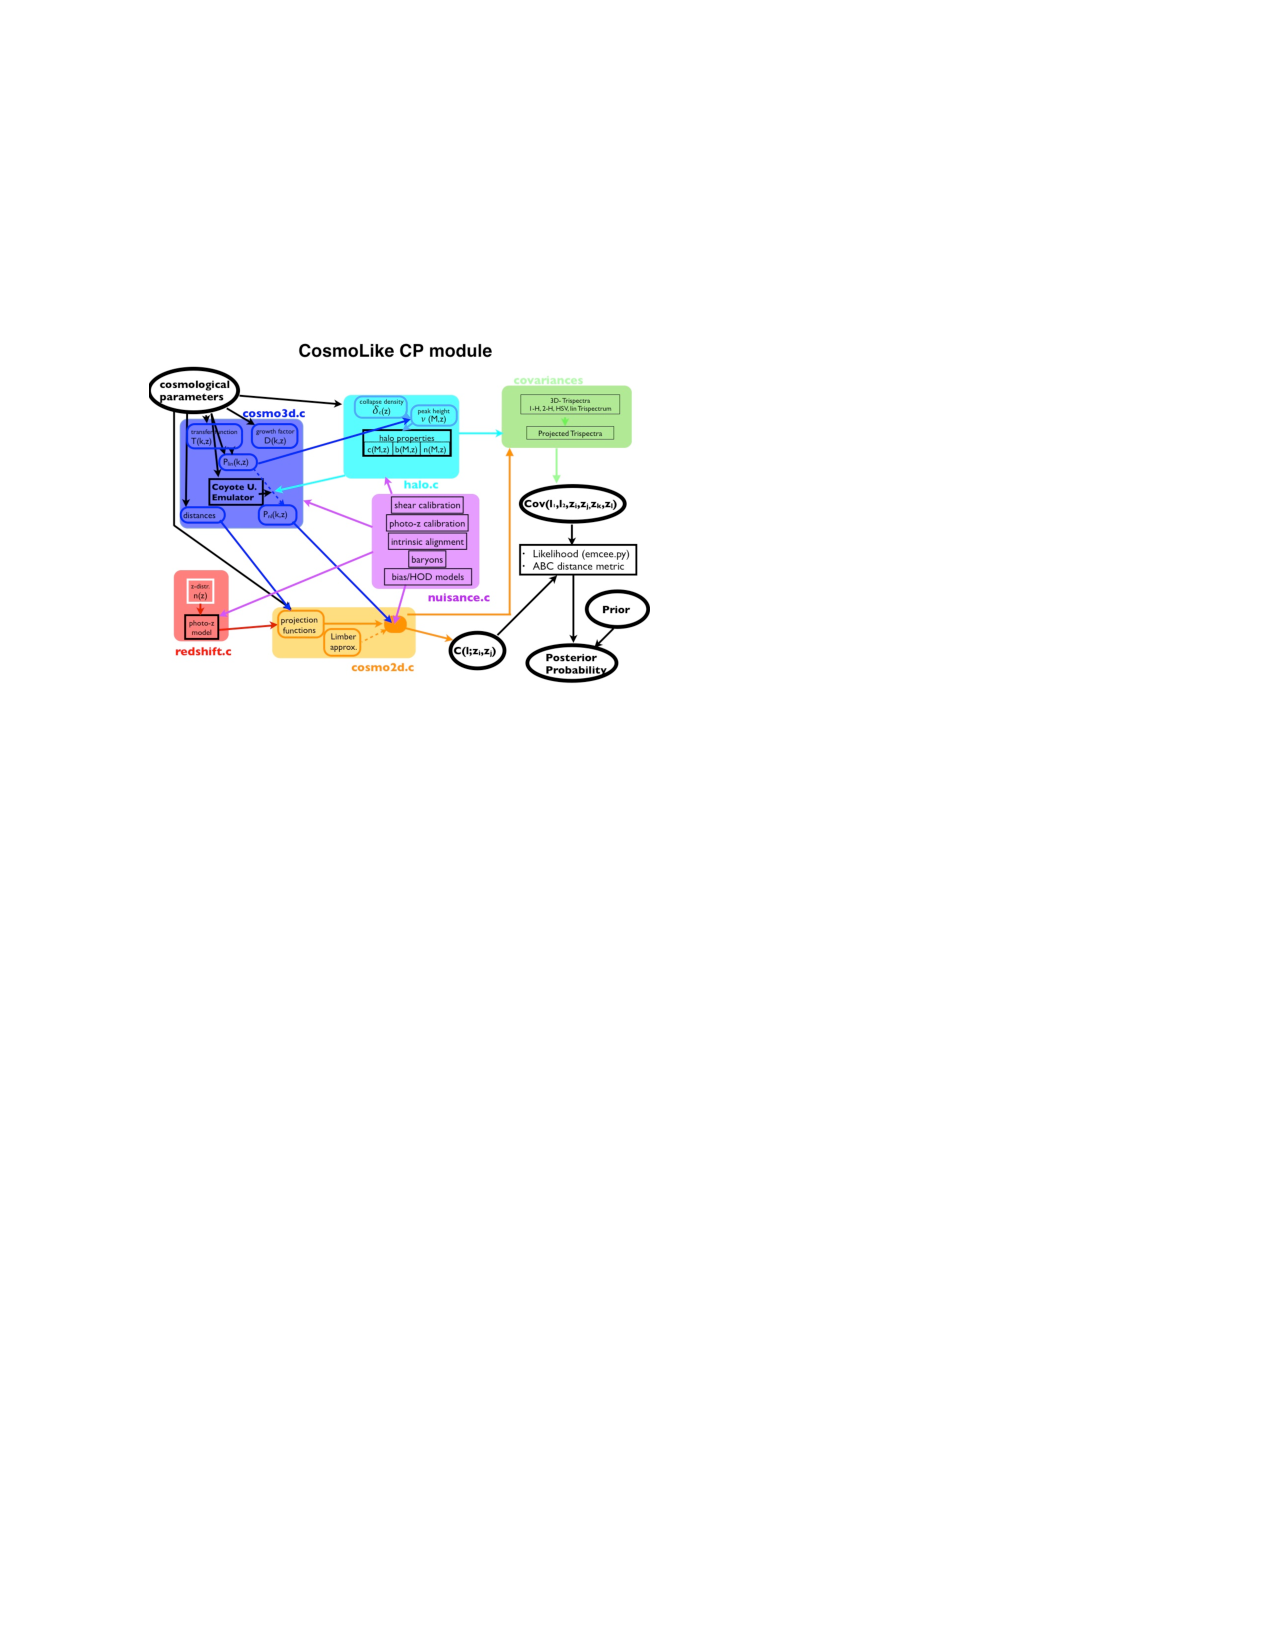
\includegraphics[width=16.0cm]{Plots/forecasts/cosmolike_codestruct}
   \caption{Illustration of a subset of CosmoLike's code structure. Starting from cosmological parameters we give details on how different parts of the code interface and how to finally obtain projected summary statistics for various observables. We note that this particular workflow represents a multi-probe analysis as described in Sect. {\ref{sec:multi-probe}}. For the HLSS survey a subset of the routines is being used.
}
  \label{fi:fcosmolike}
\end{figure*}

CosmoLike is unique in its integrated ansatz of jointly modeling LSS probes and their correlated systematics. It is the only code that computes multi-probe covariances, including the (dominant) higher-order terms of the matter density field. The code has been used to simulate realistic multi-probe likelihood analyses for LSST \citep{Krause2017} that include cosmic shear, galaxy clustering, galaxy-galaxy lensing, cluster number counts and cluster weak lensing. 
The software relies on the massively parallelized computation of fine-tuned look-up tables with a targeted sub-second run-time per point in parameter space. Given the large number of parameters describing systematic effects in future LSS analyses this efficient computation ensures an acceptable turnaround time for the analyses. In particular, it allows for the large number of simulated likelihood analyses that are needed to optimize future surveys. Figure 1 illustrates the CosmoLike combined probes module we plan to use for the proposed analysis. Starting from a cosmological model, this schematic illustrates how projected power spectra for various LSS probes are computed: 
\begin{enumerate}
\item In the first step CosmoLike computes the 3D-density power spectra using one of 3 different methods. The density power spectrum can be modeled using the latest suites of numerical simulations, i.e. the Coyote Universe emulator (Heitmann et al. 2014), or the latest implementation of Halofit (Takahashi et al. 2012), or using a state-of-the-art analytic halo model code \citep{Krause2013}. 
\item Given a survey specific redshift distribution CosmoLike computes projected (tomographic) 2D power spectra for WL, galaxy-galaxy lensing, and galaxy clustering.
\item  For the latter two probes the connection between dark and luminous matter is modeled through either a linear bias model or a sophisticated (but computationally slower) HOD implementation (Krause et al. 2013).
\item The covariance is computed analytically using perturbation theory to include the higher-order moments of the density field, including the Halo Sample Variance contribution that dominates the statistical error budget. This covariance takes all cross-correlations between the different probes into account. 
\item CosmoLike has various systematics modeling capabilities, in particular it can account for baryonic effects, intrinsic alignment, shear calibration and photo-z uncertainties \citep{Eifler2015, Krause2016, Krause2017}. 
\item If one chooses to use two-point correlation functions instead of power spectra CosmoLike offers an extremely fast Fourier transformation using a Hankel transform. As a default the code is connected to a parallel MCMC sampling technique \citep{Goodman2010}, implemented through the emcee python package \citep{Foreman-Mackey2013}.
\end{enumerate}

   
\subsection{HLSS Forecasts}
We have carried out a trade study of area versus depth for the HLSS only, starting from a baseline survey of 2227 deg2 and a wavelength range of 1.05-1.85 microns. We consider two alternative scenarios, i.e. a survey twice as wide and shallower and a survey half as wide but correspondingly deeper.  

The galaxy redshift distributions were computed using the WFIRST Exposure Time Calculator ETC v14. The H-alpha forecasts are based on the average of the 3 models in Pozzetti et al. (2016), and the [O III] forecasts are based on the Mehta et al. (2015) luminosity function. The resulting redshift distributions are visualized in Fig. 1.
We extend the CosmoLike framework (Eifler et al 2014, Krause\&Eifler 2017) to compute the constraining power of all scenarios on cosmic acceleration, closely following Wang et al (2013). We run 500,000 step MCMC simulated likelihood analysis in a 23 dimensional parameter space. We simultaneously vary 7 cosmological parameters and 16 nuisance parameters describing uncertainties due to the linear galaxy bias model, the non-linear smearing of the BAO feature, peculiar velocity dispersion, power spectrum shot noise, and redshift errors. We assume priors on cosmological parameters from the current state of the art experiments, i.e. the Planck mission, the Baryon Oscillation Spectroscopic Survey, the Joint Lightcurve Analysis, as described in Aubourg et al (2015). 

The information gain is quantified using the standard Dark Energy Task Force FOM and an extended cosmology FOM, which measures the enclosed volume in the full 7-dimensional cosmological parameter space, not just in the 2 dark energy parameters. We will refer to these FOMs as DE-FOM and Cosmo-FOM. 
Compared to our baseline scenarios we find a decreased DE-FOM of 32\% and a decreased Cosmo-FOM of 45\% for the shallow/large area survey. For the deep/small area survey we find an increased DE-FOM of 5\% and an increased Cosmo-FOM of 2\%. We note that these findings are model and prior dependent and recommend further studies varying these input parameters. We also note that the [O III] numbers are pending a future update in part due to the reduction in the baseline telescope temperature to 260 K.
\begin{figure*}
  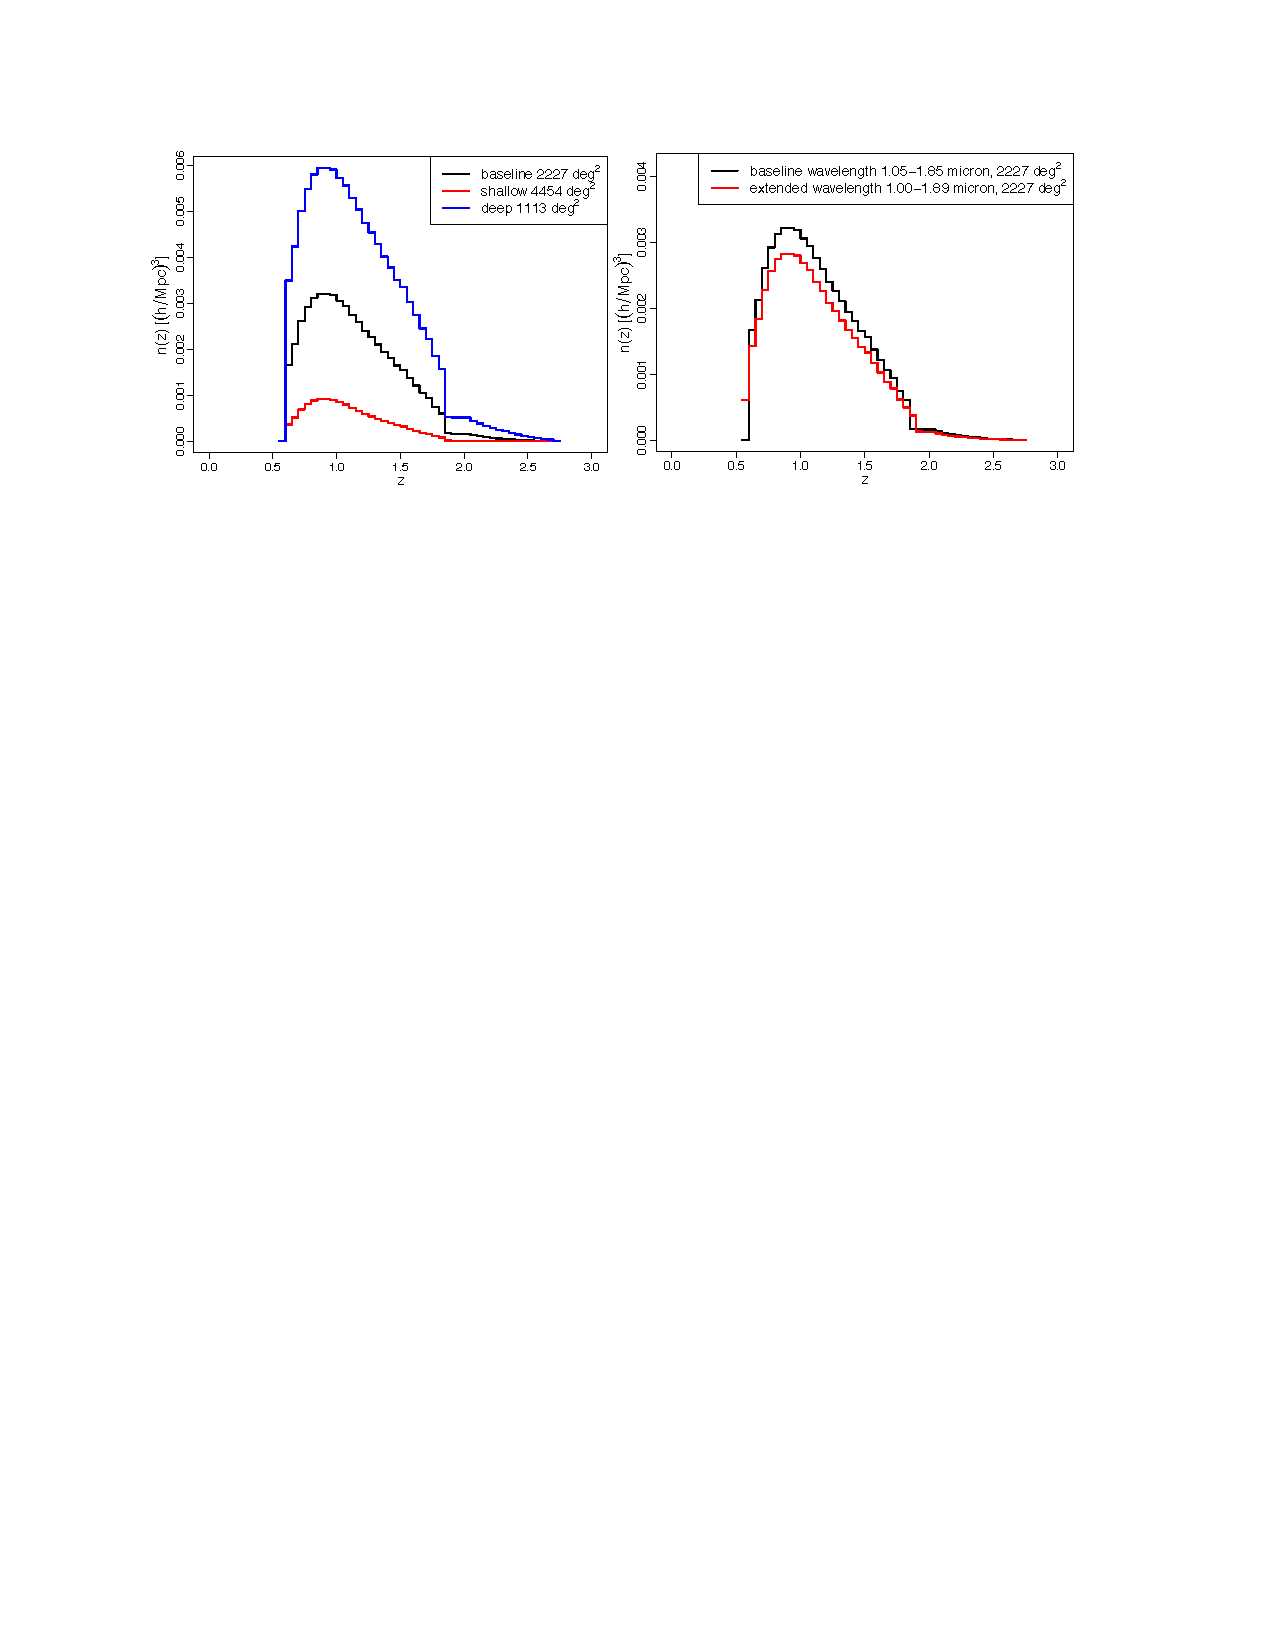
\includegraphics[width=16.0cm]{Plots/forecasts/HLSS_forecasts}
    \caption{\textit{Left:}Redshift distribution of galaxies of the baseline, the shallow/large area and the deep/small area survey. \textit{Right:} Redshift distribution of galaxies of the baseline and extended wavelength survey. 
}
  \label{fi:forecast1}
\end{figure*}

HLSS 3: The redshift range of galaxies surveyed shall encompass 1. $\leq$ z $\leq$ 2.7 


In addition to the trade studies in HLSS 1 we examine the impact of an extended wavelength range on the DE-FOM and the Cosmo-FOM. We follow the same procedure as detailed in the HLSS 1 paragraph extending the wavelength range from 1.05-1.85 microns for the baseline model to 1.00-1.89 for the extended model. The corresponding redshift distributions of the galaxy samples computed from the ETC v1.14 are depicted in Fig. 2. We find a decreased DE-FOM of 2\% and a decreased Cosmo-FOM of 11\% for the extended wavelength survey with respect to our baseline scenario. We iterate that these findings are model and prior dependent and recommend further studies varying these input parameters.

%%%%%%%%%%%%%%%%%%%%%%%%%%%%%%%%%%%
\subsection{HLIS Forecasts}
\label{sec:HLISforecasts}
%%%%%%%%%%%%%%%%%%%%%%%%%%%%%%%%%%%
\begin{figure*}
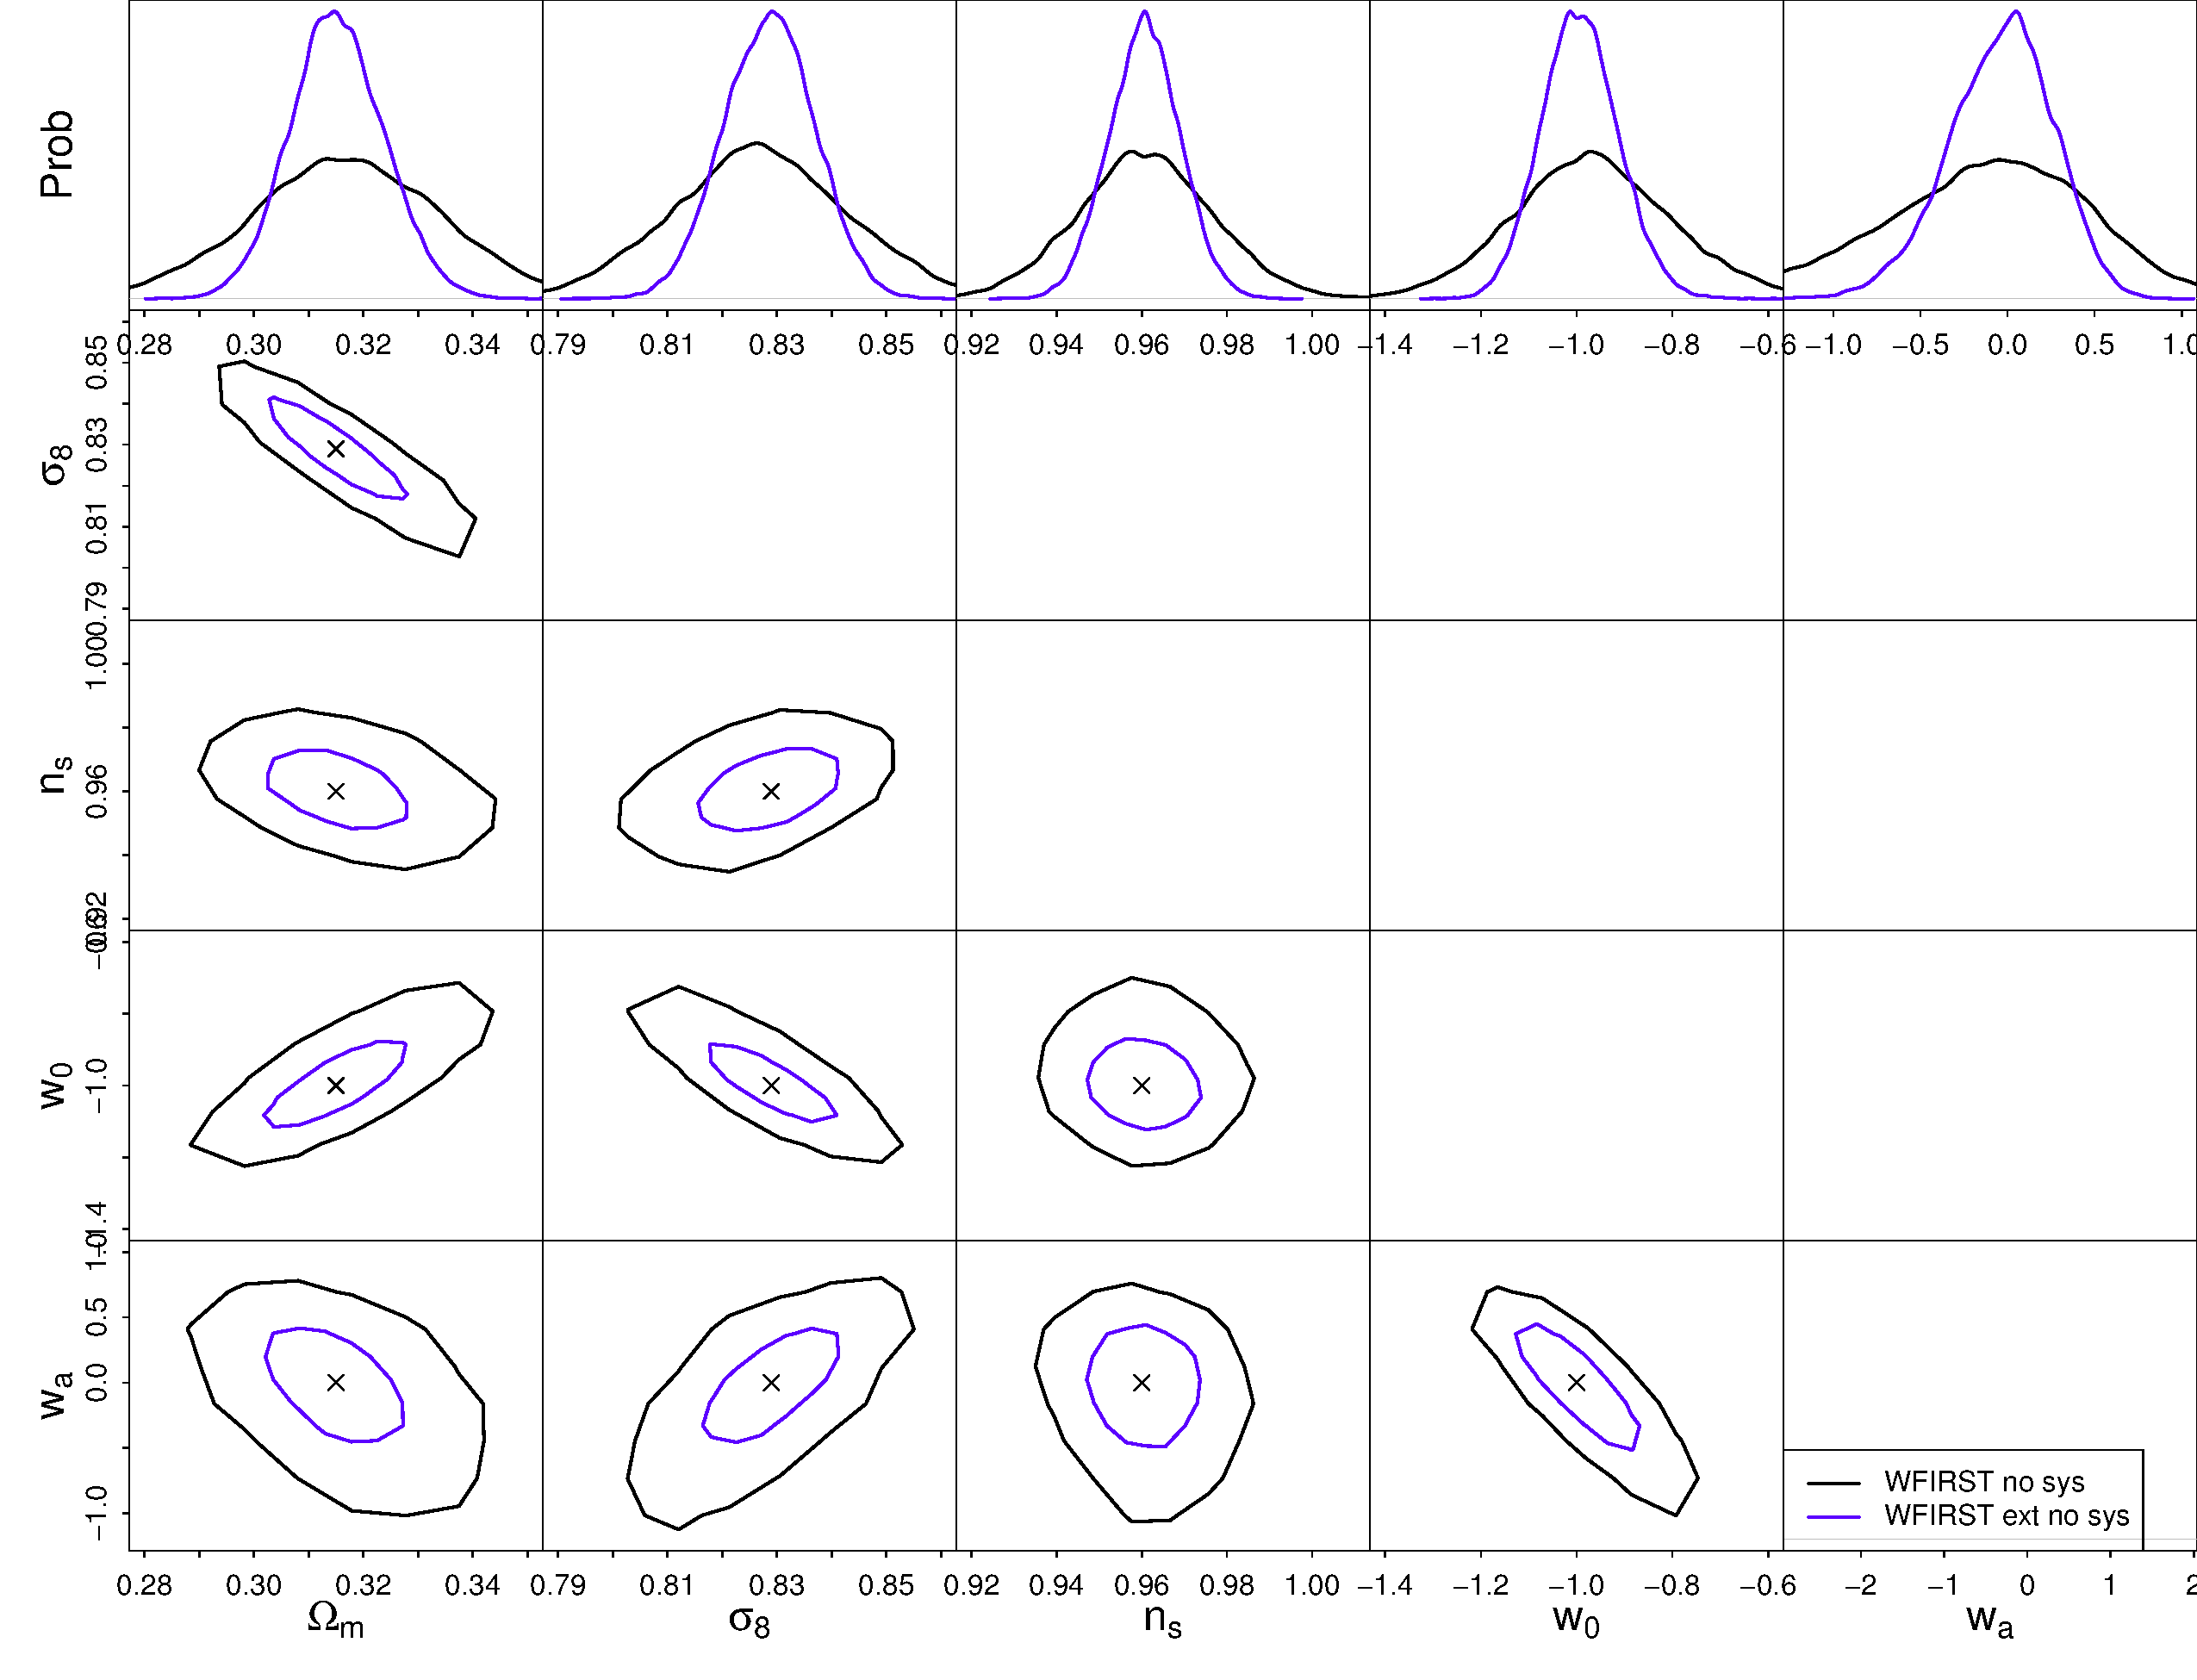
\includegraphics[width=14cm]{Plots/forecasts/WFIRST_no_sys.eps}
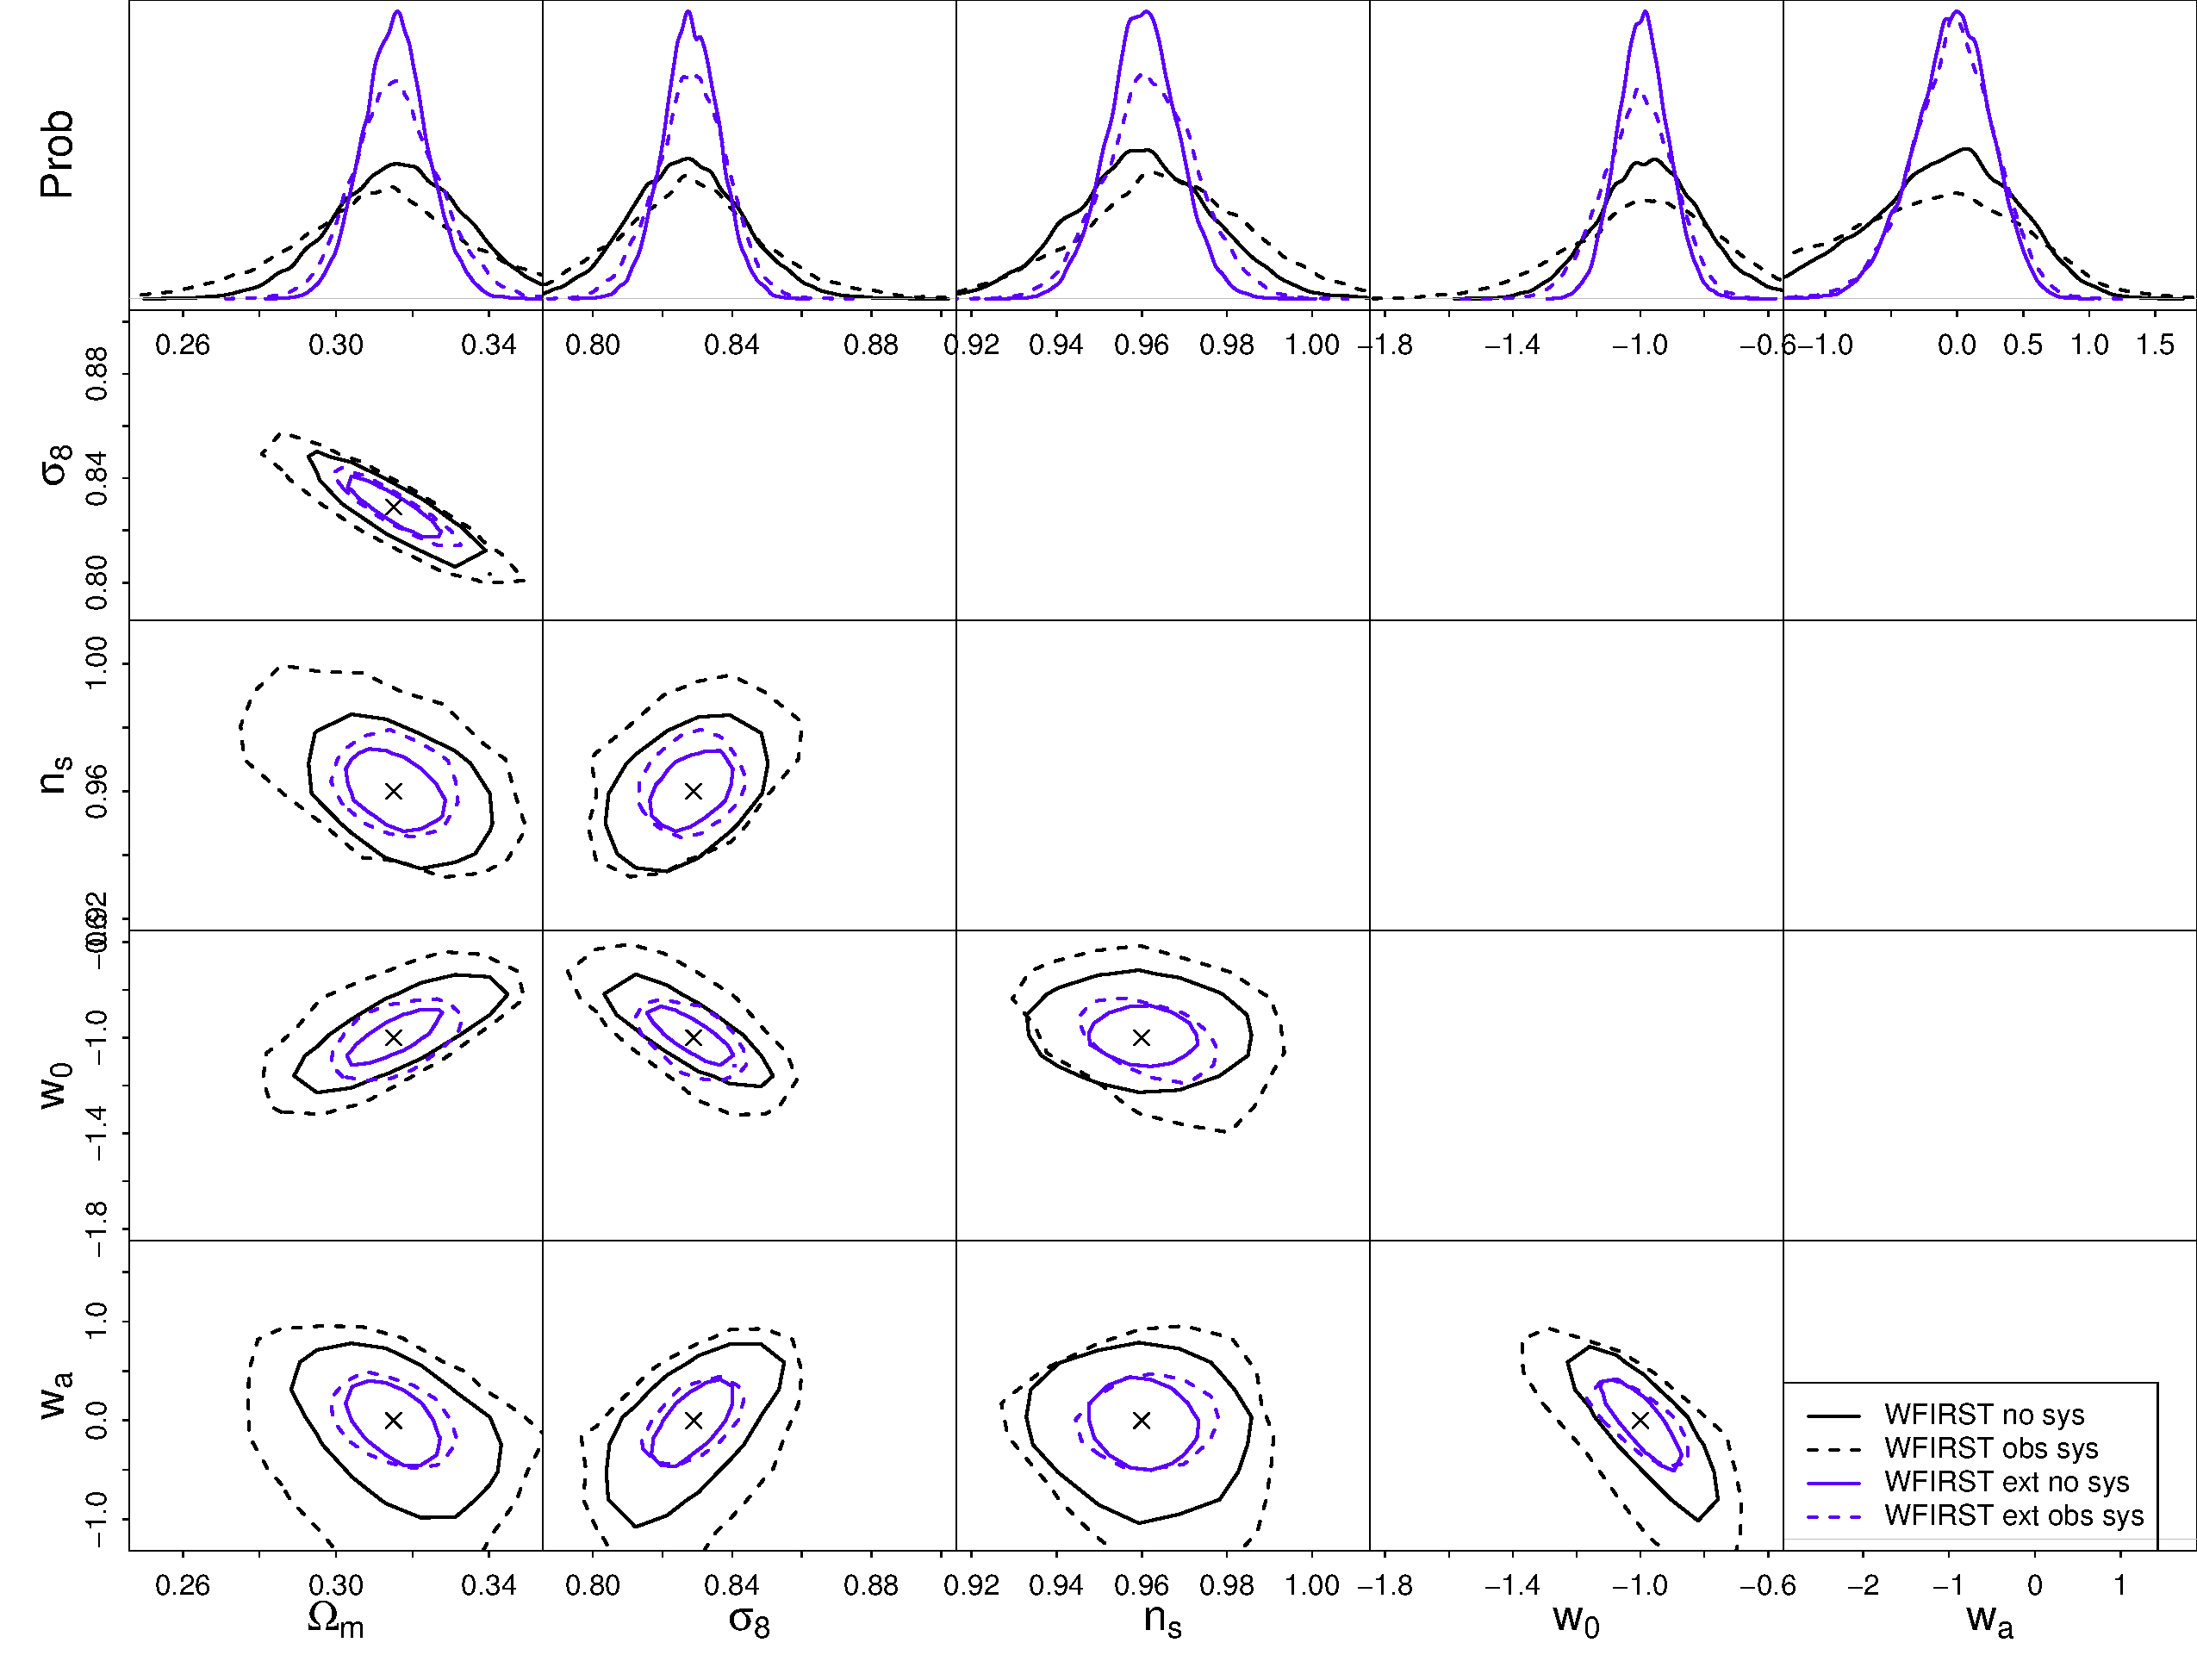
\includegraphics[width=14cm]{Plots/forecasts/WFIRST_obs_sys.eps}
\caption{\textit{Top:} WFIRST forecasts statistical errors only. Extended Mission 10,000 $\mr{deg^2}$ in blue, regular mission 2200 $\mr{deg^2}$ in black. \textit{Bottom:} Broadening of WFIRST error bars accounting for shear calibration and photo-z errors.}
         \label{fi:extended}
\end{figure*}

\begin{figure*}
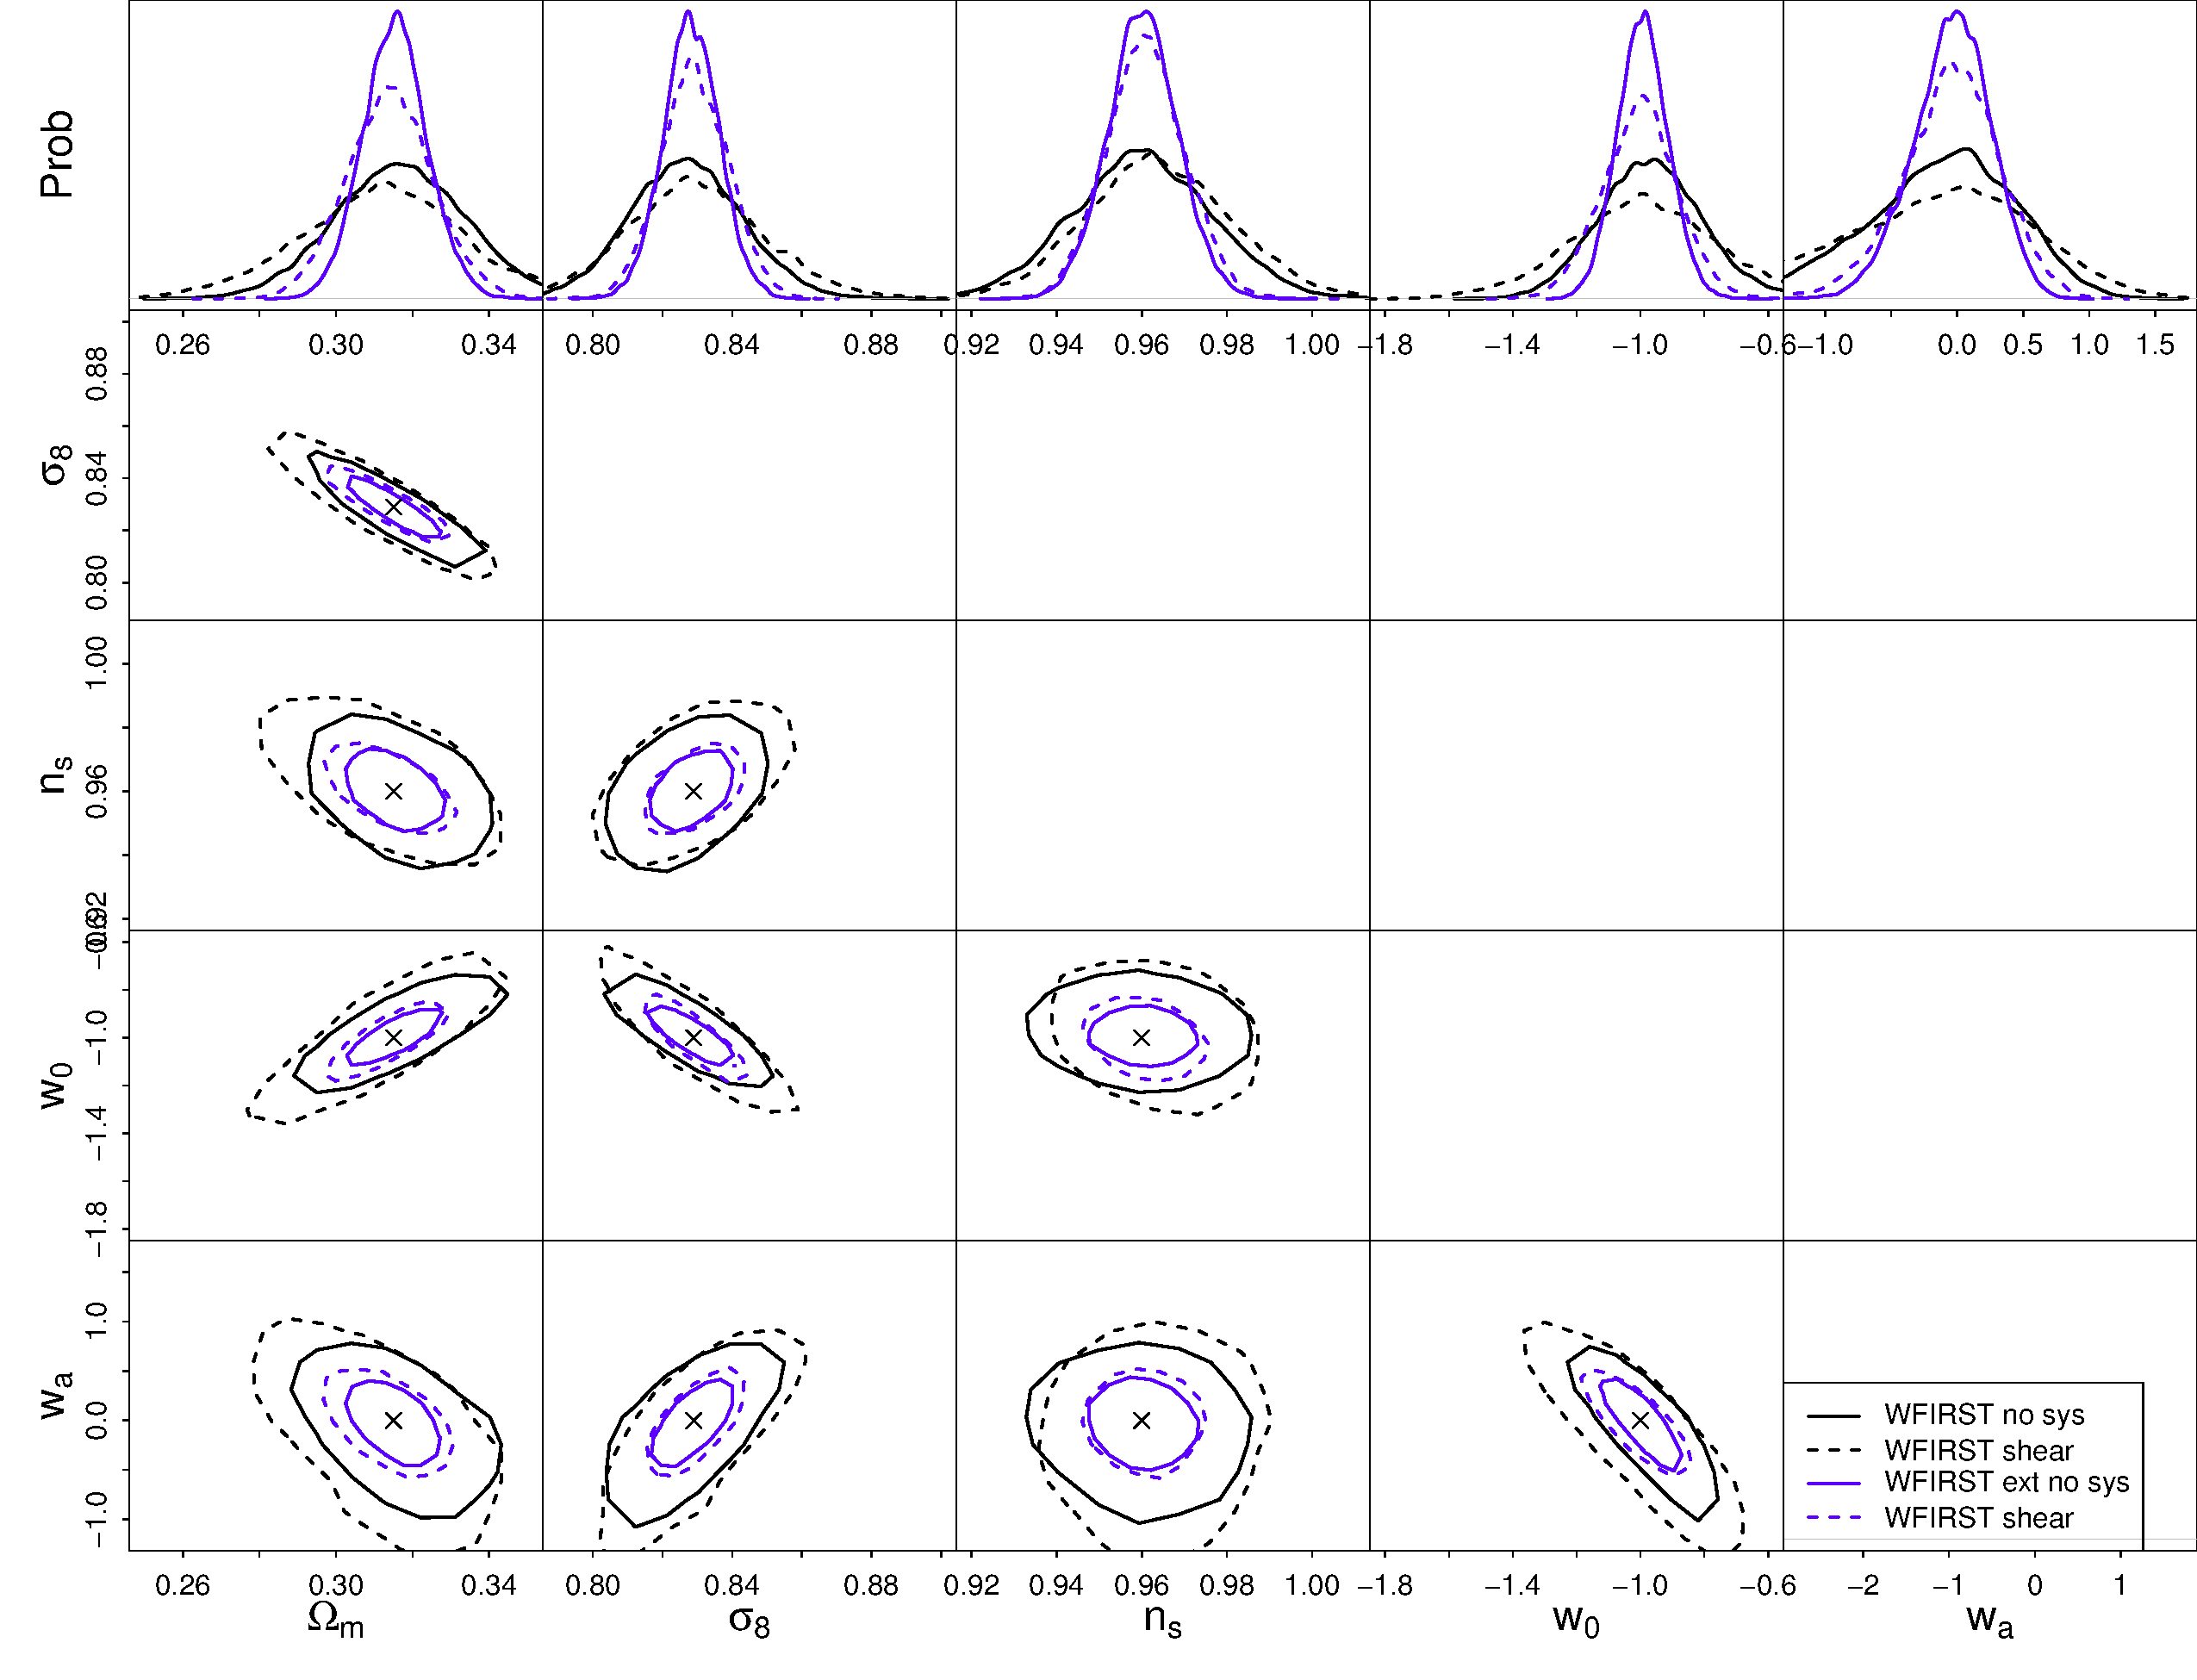
\includegraphics[width=14cm]{Plots/forecasts/WFIRST_shear.eps}
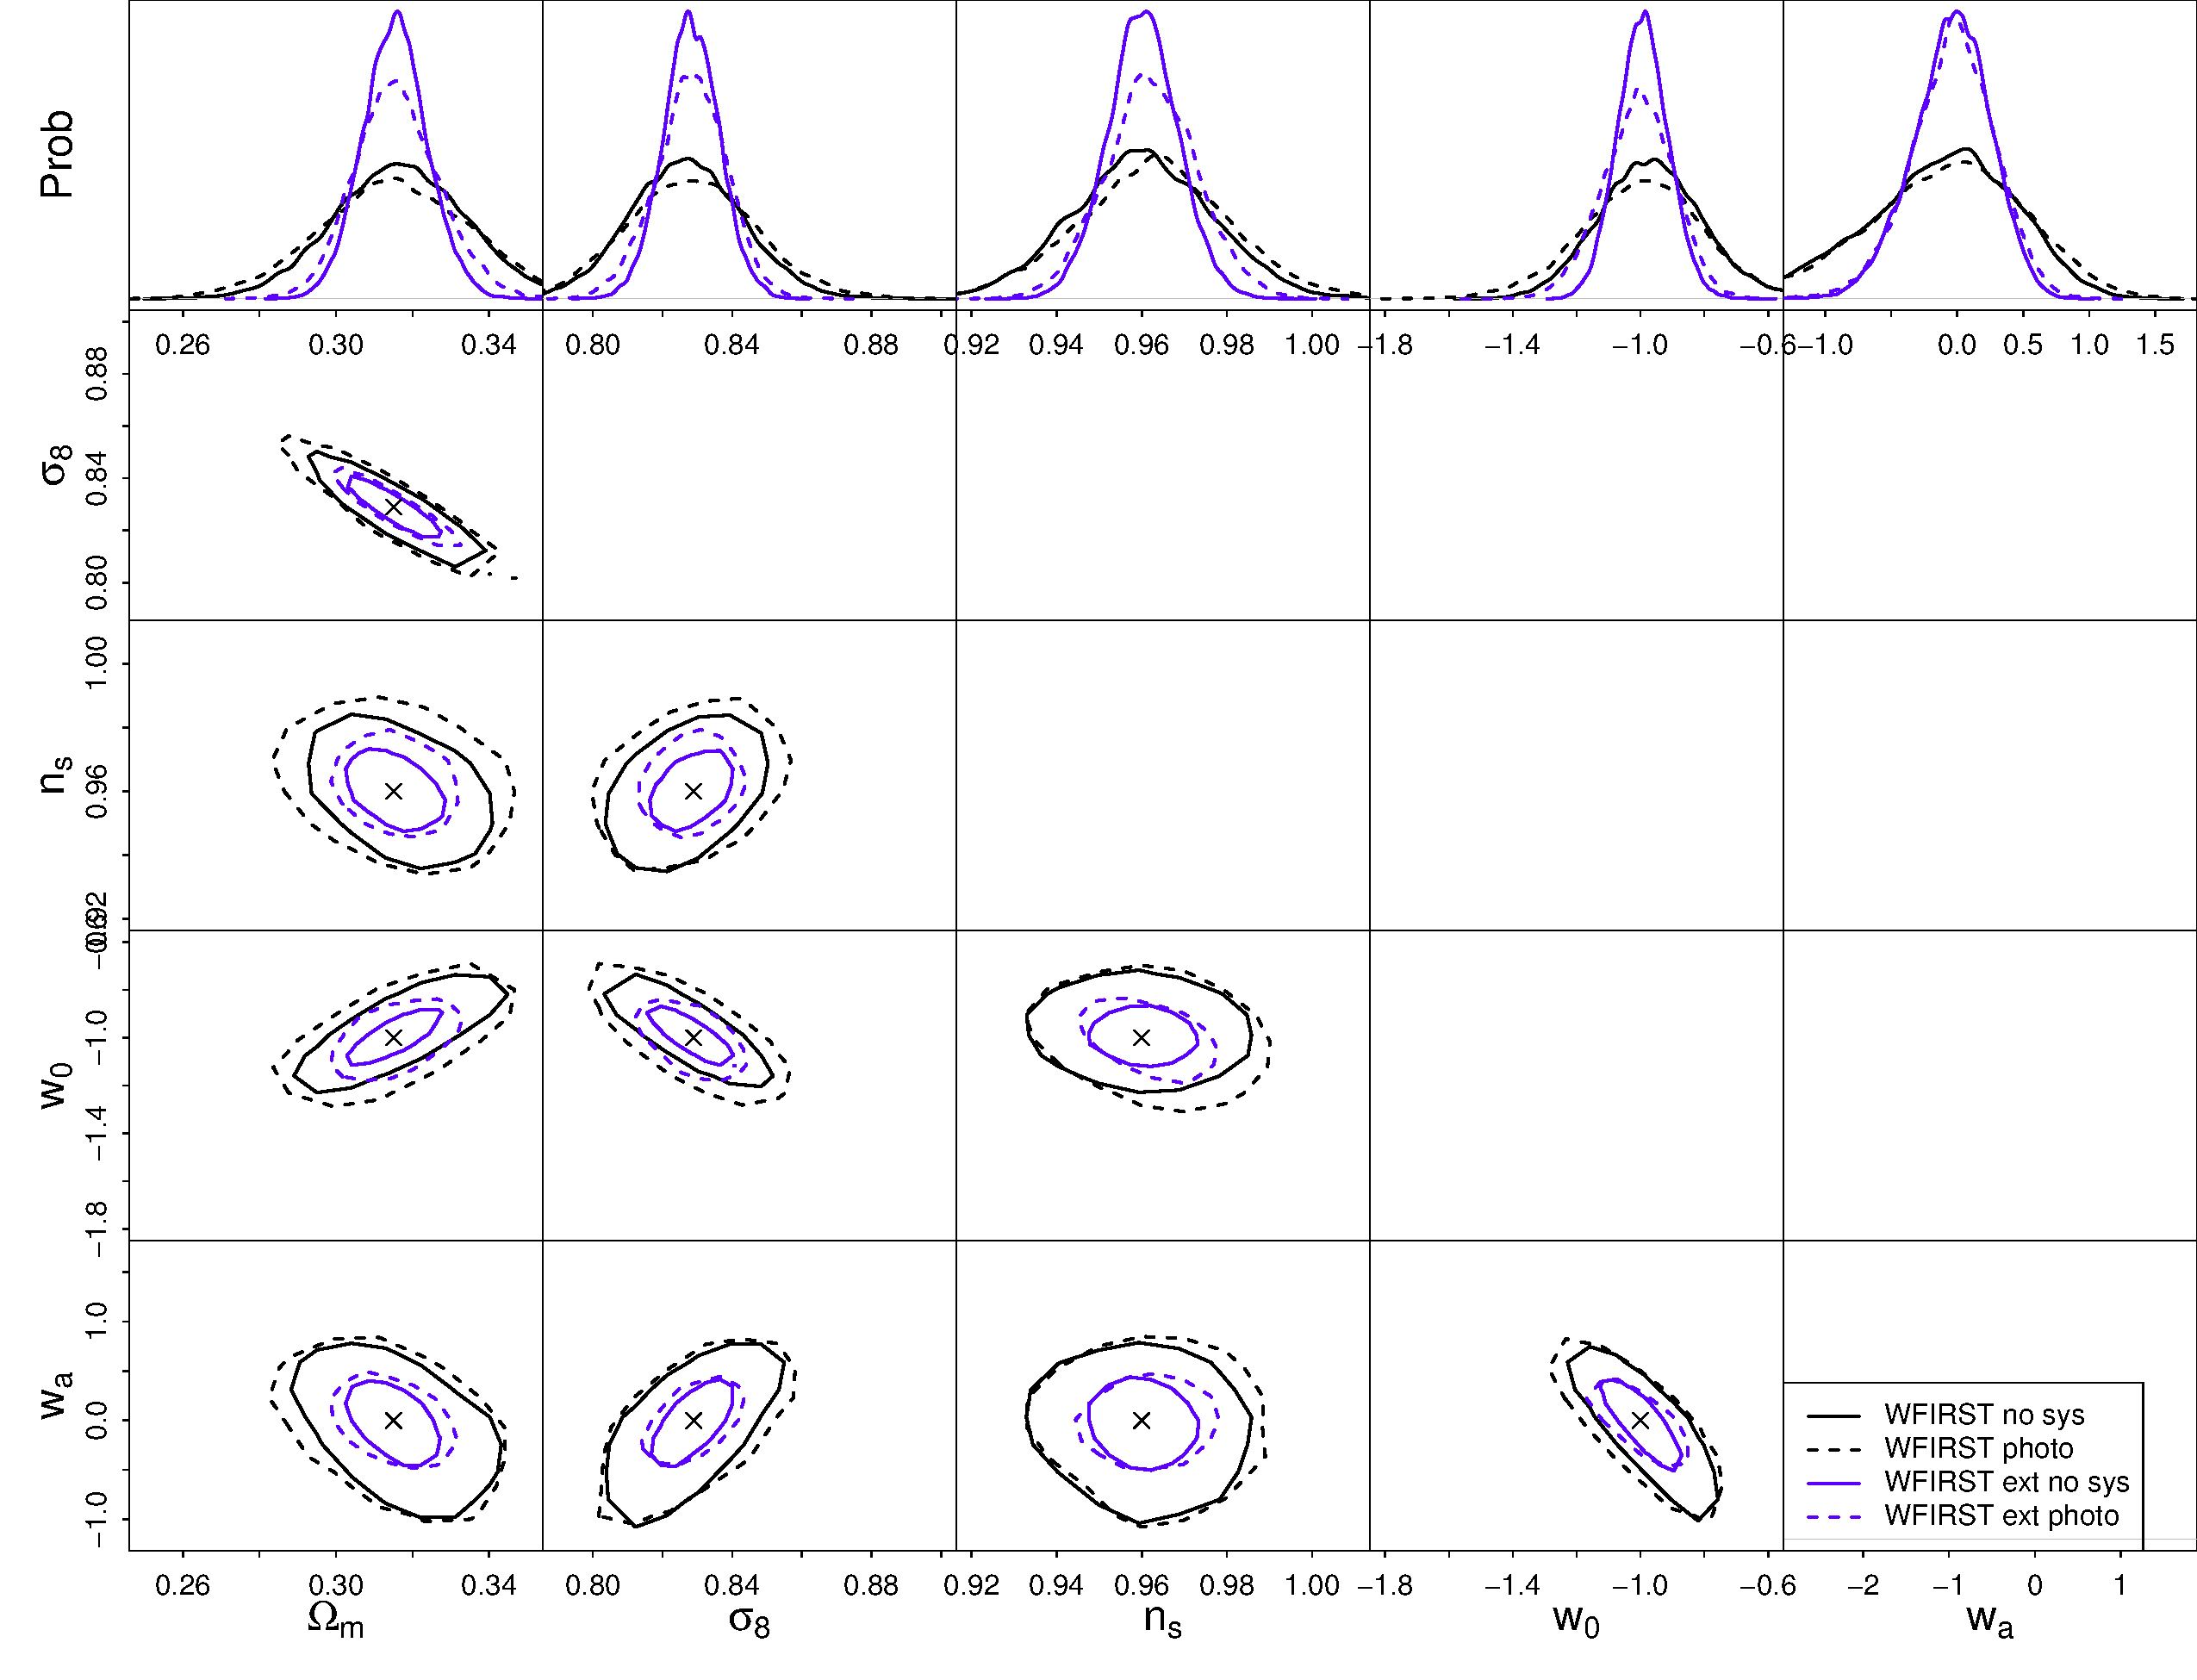
\includegraphics[width=14cm]{Plots/forecasts/WFIRST_photo.eps}
\caption{\textit{Top:} WFIRST forecasts statistical errors (solid) compared to errors when including uncertainties from multiplicative shear calibration errors (dashed).  Extended Mission 10,000 $\mr{deg^2}$ in blue, regular mission $2200 \mr{deg^2}$ in black
\textit{Bottom:} WFIRST contours when accounting for photo-z uncertainties; see text for details.}
         \label{fi:sys_obs}
\end{figure*}

\begin{figure*}
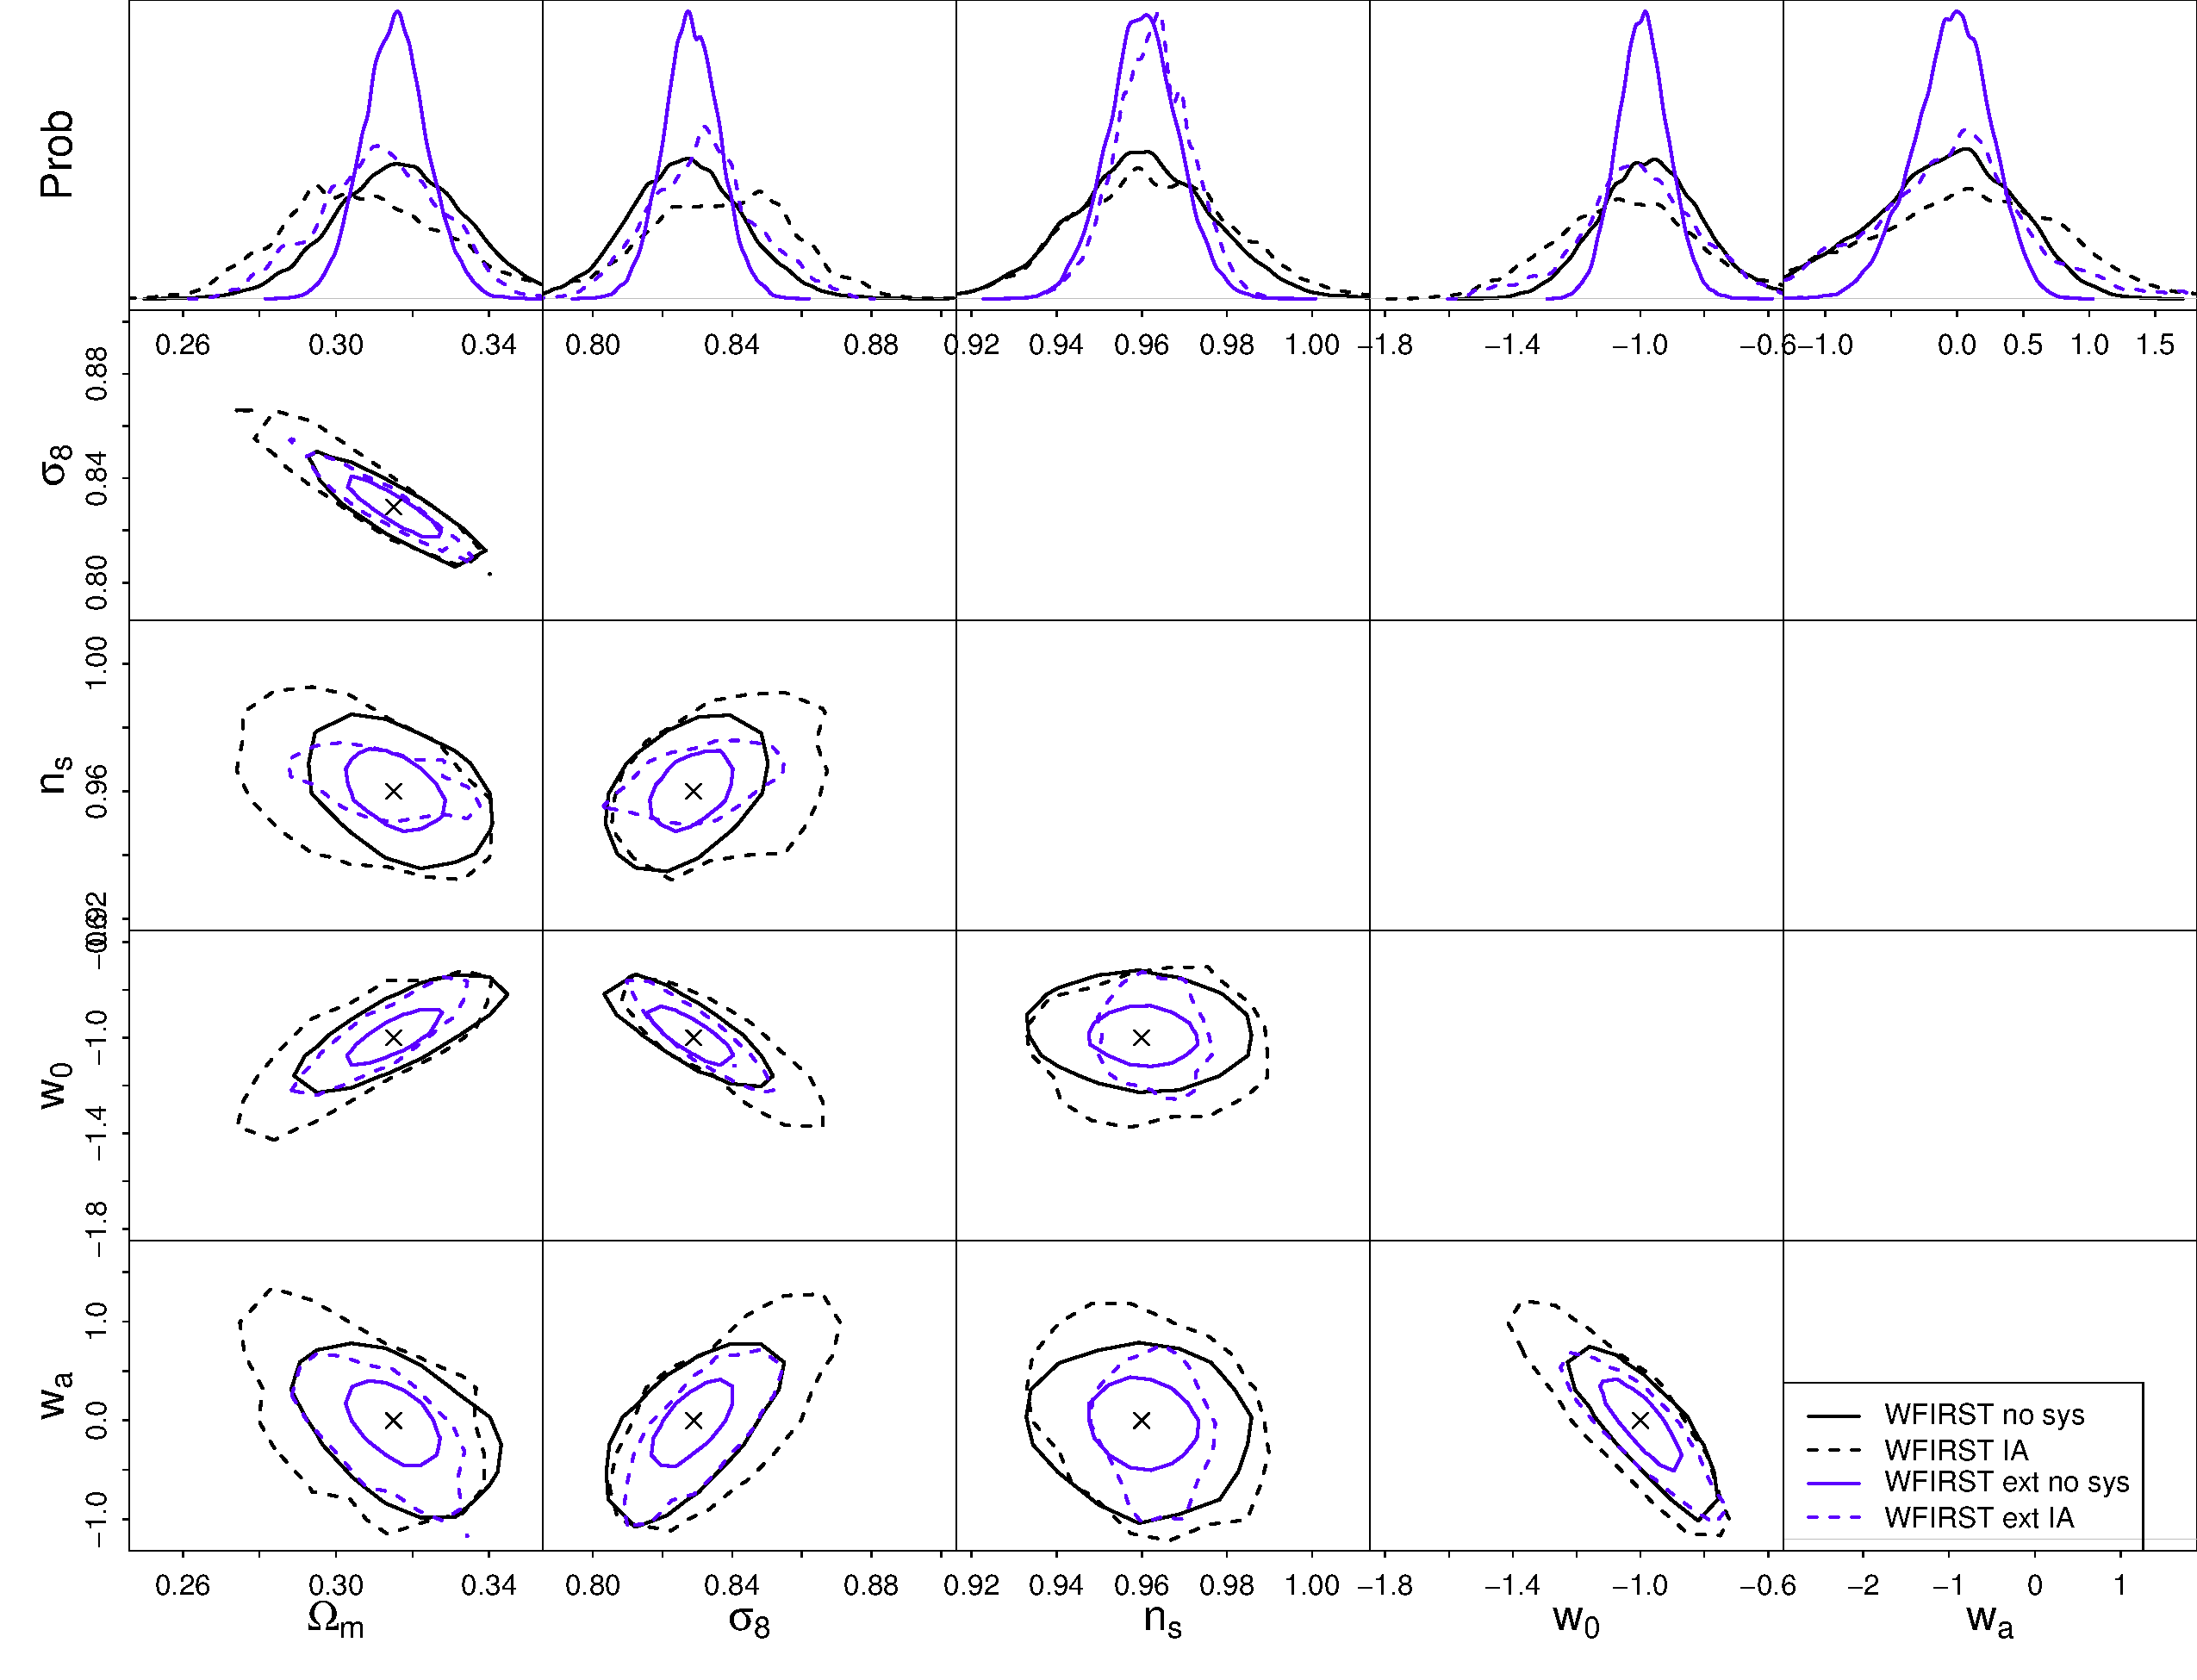
\includegraphics[width=14cm]{Plots/forecasts/WFIRST_ia.eps}
\caption{Increase of WFIRST (nominal and extended mission) error bars when marginalizing over intrinsic alignment nuisance parameters \citep[see][for comparison]{keb16}.}
         \label{fi:IA}
\end{figure*}

\begin{figure*}
\includegraphics[width=14cm]{Plots/forecasts/WFIRST_bary_impact.eps}
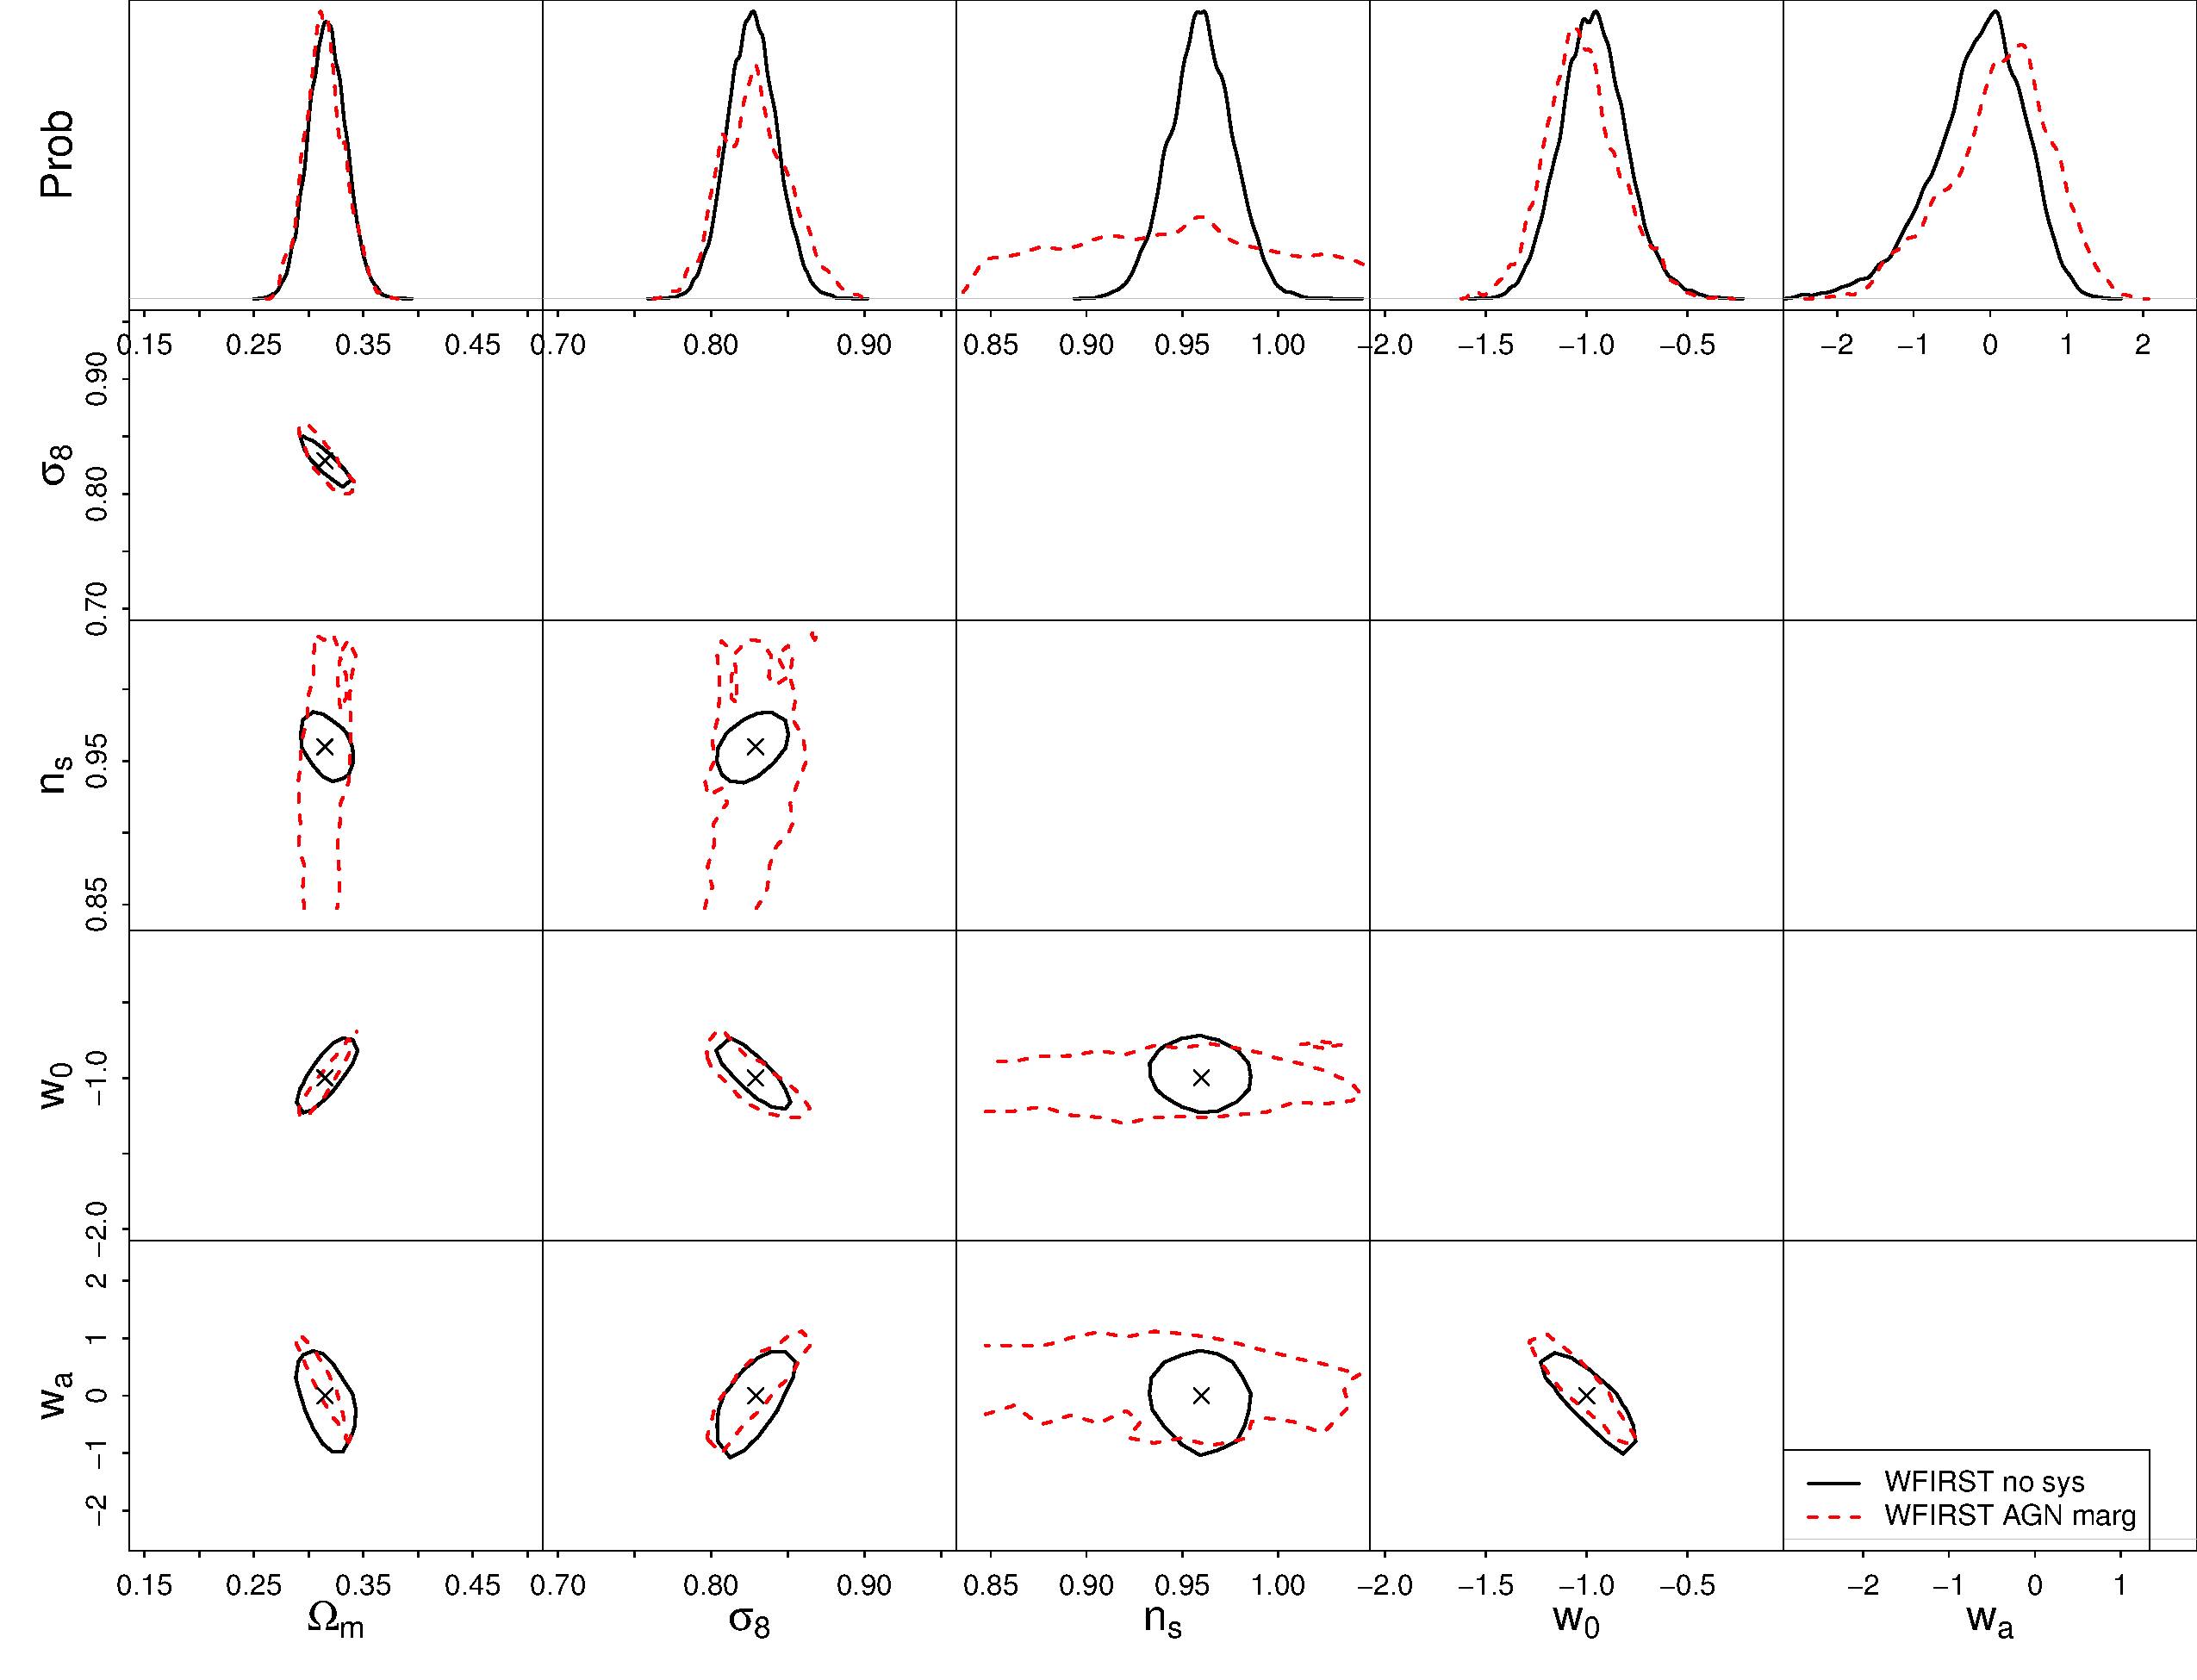
\includegraphics[width=14cm]{Plots/forecasts/WFIRST_bary_miti.eps}
\caption{Increase of WFIRST (nominal and extended mission) error bars when marginalizing over nuisance parameters modeling baryonic physics \citep[see][for details of the method]{ekd15}.}
         \label{fi:bary}
\end{figure*}

We begin the WFIRST HLIS section by forecasting the weak lensing science component only. We closely follow the weak lensing part of the forecasting machinery described in \cite{Krause17}. 

\subsection{Modelling Weak lensing observables and covariances}
\label{sec:lensingbasics}

\paragraph*{Shear tomography power spectra}
\textsc{CosmoLike} obtains matter power spectra through calls to the Boltzmann code \textsc{CLASS} code \citep{CLASS}and it uses the \citet{tsn12} calibration of the \textsc{halofit} fitting function for the non-linear matter power spectrum \citep{smp03}, Time-dependent dark energy models ($w=w_0+(1-a)\,w_a$) are incorporated following the recipe of {\sc icosmo} \citep{rak11}, which in the non-linear regime interpolates Halofit between flat and open cosmological models \citep[also see][for more details]{shj10}.

Having obtained the density power spectra we calculate the shear power spectra as
\begin{equation}
\label{eq:pdeltatopkappa}
C ^{ij} (l) = \frac{9H_0^4 \om^2}{4c^4} \int_0^{\chi_\mr h} 
\mr d \chi \, \frac{g^{i}(\chi) g^{j}(\chi)}{a^2(\chi)} \pd \left(\frac{l}{f_K(\chi)},\chi \right) \,,
\end{equation}
with $l$ being the 2D wave vector perpendicular to the line of sight, $\chi$ denoting the comoving coordinate, $\chi_\mr h$ is the comoving coordinate of the horizon, $a(\chi)$ is the scale factor, and $f_K(\chi)$ the comoving angular diameter distance (throughout set to $\chi$ since we assume a flat Universe). The lens efficiency $g^{i}$ is defined as an integral over the redshift distribution of source galaxies $n(\chi(z))$ (see Sect. \ref{sec:surveys} fro details) in the $i^\mr{th}$ tomographic interval
\begin{equation}
\label{eq:redshift_distri}
g^{i}(\chi) = \int_\chi^{\chi_{\mr h}} \mr d \chi' n^{i} (\chi') \frac{f_K (\chi'-\chi)}{f_K (\chi')} \,.
\end{equation}
Since we chose five tomographic bins, the resulting data vector which enters the likelihood analysis consists of 15 tomographic shear power spectra, each with 12 logarithmically spaced bins ($l \in [100;5000]$), hence 180 data points overall. The limits of the tomographic $z$-bins are chosen such that each bin contains a similar number of galaxies.


\paragraph*{Shear covariances}

Under the assumption that the 4pt-function of the shear field can be expressed in terms of 2pt-functions (so-called Gaussian shear field) the covariance of projected shear power spectra can be calculated as in \citep{huj04} 
\be
\label{eq:covhujain}
\mr{Cov_G} \left( C^{ij} (l_1) C^{kl} (l_2) \right) = \langle \Delta C^{ij} (l_1) \, \Delta C^{kl} (l_2) \rangle  =  \frac{\delta_{l_1 l_2}}{ 2 f_\mr{sky} l_1 \Delta l_1}  \left[\bar C^{ik}(l_1) \bar C^{jl}(l_1) + \bar C^{il}(l_1) \bar C^{jk} (l_1) \right]\,,
\ee

with
\be
\label{details}
\bar C^{ij}(l_1)= C^{ij}(l_1)+ \delta_{ij} \frac{\sigma_\eps^2}{n^{i}} \,,
\ee
where the superscripts indicate the redshift bin; $n^{i}$ is the density of source galaxies in the $i$-th redshift bin; and $\sigma_\eps$ is the RMS of the shape noise.

Since non-linear structure growth at late time induces significant non-Gaussianities in the shear field, using the covariance of Eq.~(\ref{eq:covhujain}) in a likelihood analysis results in underestimates of the errors on cosmological parameters. Therefore, the covariance must be amended by an additional term, i.e. $\mr{Cov}=\mr{Cov_G}+\mr{Cov_{NG}}$.  The non-Gaussian covariance is calculated from the convergence trispectrum $T_{\kappa}$ \citep{CH01,taj09}, and we include a sample variance term $T_{\kappa,\rm{HSV}}$ that describes scatter in power spectrum measurements due to large scale density modes \citep{tb07, sht09},
\be
 \mr{Cov_{NG}}(C^{ij}(l_1),C^{kl}(l_2)) =  \int_{|\mathbf l|\in l_1}\frac{d^2\mathbf l}{A(l_1)}\int_{|\mathbf l'|\in l_2}\frac{d^2\mathbf l'}{A(l_2)} \left[\frac{1}{\Omega_{\mr s}}T_{\kappa,0}^{ijkl}(\mathbf l,-\mathbf l,\mathbf l',-\mathbf l') + T_{\kappa,\rm{HSV}}^{ijkl}(\mathbf l,-\mathbf l,\mathbf l',-\mathbf l') \right] \,,
\ee
with $A(l_i) = \int_{|\mathbf l|\in l_i}d^2\mathbf l \approx 2 \pi l_i\Delta l_i$ the integration area associated with a power spectrum bin centered at $l_i$ and width $\Delta l_i$.

The convergence trispectrum $T_{\kappa,0}^{ijkl}$ is, in the absence of finite volume effects, defined as  
\be
\label{eq:tri2}
T_{\kappa,0}^{ijkl} (\mathbf l_1,\mathbf l_2,\mathbf l_3,\mathbf l_4) = \left( \frac{3}{2} \frac{H_0^2}{c^2} \om \right)^{4} \int_0^{\chi_h} \d \chi \, \left( \frac{\chi}{a(\chi)}\right)^4  g^i g^j g^k g^l \times \chi^{-6} \, T_{\delta,0}  \left( \frac{\mathbf l_1}{\chi}, \frac{\mathbf l_2}{\chi}, \frac{\mathbf l_3}{\chi}, \frac{\mathbf l_4}{\chi}, z(\chi) \right) \,,
\ee
with $T_{\delta,0}$ the matter trispectrum (again, not including finite volume effects), and where we abbreviated $g^i=g^i(\chi)$.

We model the matter trispectrum using the halo model \citep{Seljak00, CS02}, which assumes that all matter is bound in virialized structures that are modeled as biased tracers of the density field. Within this model the statistics of the density field can be described by the dark matter distribution within halos on small scales, and is dominated by the clustering properties of halos and their abundance on large scales. In this model, the trispectrum splits into five terms describing the 4-point correlation within one halo (the \emph{one-halo} term $T^{\mr{1h}}$), between 2 to 4 halos (\emph{two-, three-, four-halo} term), and a so-called halo sample variance term $T_{\mr{HSV}}$, caused by fluctuations in the number of massive halos within the survey area,
\be
\label{eq:t}
T = T_0 + T_{\mr{HSV}} = \left[T_{\mr{1h}}+T_{\mr{2h}}+T_{\mr{3h}}+T_{\mr{4h}}\right]+T_{\mr{HSV}}\;.
\ee
The \emph{two-halo} term is split into two parts, representing correlations between two or three points in the first halo and two or one point in the second halo. As halos are the building blocks of the density field in the halo approach, we need to choose models for their internal structure, abundance and clustering in order to build a model for the trispectrum. 


Our implementation of the one-, two- and four-halo term contributions to the matter trispectrum follows \citet{CH01}, and we neglect the three-halo term as it is subdominant compared to the other terms at the scales of interest for this analysis. Specifically, we assume NFW halo profiles \citep{NFW} with the \citet{Bhattacharya11} fitting formula for the halo mass--concentration relation $c(M,z)$, and the \citet{Tinker10} fit functions for the halo mass function $\frac{ dn}{dM}$ and linear halo bias $b(M)$ (all evaluated at $\Delta = 200$), neglecting terms involving higher order halo biasing.


Within the halo model framework, the halo sample variance term is described by the change of the number of massive halos within the survey area due to survey-scale density modes; following \citet{sht09} it is calculated as

\begin{eqnarray}
T_{\kappa,\rm{HSV}}^{ijkl}(\mathbf l_1,-\mathbf l_1,\mathbf l_2,-\mathbf l_2)= \left(\frac{3}{2}\frac{H_0^2}{c^2}\Omega_{\mr m}\right)^4 &\times&  \int_0^{\chi_\mr h}d\chi \left(\frac{d^2 V}{d\chi d\Omega}\right)^2 \left(\frac{\chi}{a(\chi)}\right)^4 g^i g^j g^k g^l \nn \\
&\times&  \int d M \frac{d n}{d M} b(M)\left(\frac{M}{\bar{\rho}}\right)^2 |\tilde{u}(l_1/\chi, c(M,z(\chi))|^2 \nn \\
 &\times& \int d M' \frac{d n}{d M'} b(M')\left(\frac{M'}{\bar{\rho}}\right)^2 |\tilde{u}(l_2/\chi, c(M',z(\chi))|^2 \nn \\
 &\times&  \int_0^\infty \frac{k dk}{2\pi}P_\delta^{\mr{lin}}(k,z(\chi))|\tilde W(k\chi \Theta_{\mr s})|^2 \,.
\end{eqnarray}


\paragraph* {Parameter studies}
Given our capability to model shear power spectra and non-Gaussian covariances we can embark on forecasting several survey scenarios and study the impact of systematics. For all forecasts we sample the joint parameter space of cosmological $\pco$ and nuisance parameters $\pnu$ and parameterize the joint likelihood as a multivariate Gaussian 
\be
\label{eq:like}
\like (\D| \pco, \pnu) = N \, \times \, \exp \biggl( -\frac{1}{2} \underbrace{\left[ (\D -\M)^t \, \matC^{-1} \, (\D-\M) \right]}_{\chi^2(\pco, \pnu)}  \biggr) \,.
\ee
The model vector $\M$ is a function of cosmology and nuisance parameters, i.e. $\M=\M(\pco, \pnu)$ and the normalization constant $N=(2 \pi)^{-\frac{n}{2}} |C|^{-\frac{1}{2}}$ can be ignored under the assumption that the covariance is constant in parameter space. The assumption of a constant, known covariance matrix $\matC$ is an approximation to the correct approach of a cosmology dependent or estimated covariance \citep[see][for further details]{esh09, seh15}.     
Given the likelihood function we can compute the posterior probability in parameter space from Bayes' theorem
\be
\label{eq:bayes}
\prob(\pco, \pnu|\D) \propto \probr (\pco, \pnu) \,\like (\D| \pco, \pnu),
\ee
where $\probr (\pco, \pnu)$ denotes the prior probability.

Equation \ref{eq:bayes} and above allow us to simulate realistic likelihood analyses for various WFIRST survey aspects, in particular we consider the following scenarios:
\begin{itemize}
\item Science gain when extending the survey to 10,000 deg$^2$, instead if 2,200 deg$^2$ (see Fig \ref{fi:extended} top)
\item Impact of uncertainties in shape measurements and photo-z measurements in combination (see Fig \ref{fi:extended} bottom)
\item Impact of uncertainties in shape measurements only (see Fig \ref{fi:sys_obs} top)
\item Impact of uncertainties in photo-z estimation only (see Fig \ref{fi:sys_obs} bottom)
\item Impact of uncertainties in baryonic physics modeling (see Fig \ref{fi:bary} bottom)
\item Impact of uncertainties in intrinsic alignment modeling (see Fig \ref{fi:IA} bottom) 
\end{itemize}

Shear calibration uncertainties are modeled as a Gaussian with $\sigma=0.005$ in each of the 10 tomographic bins, which altogether accumulates to 11 nuisance parameters. Redshift errors are modeled as Gaussian errors with a bias around mean zero and $\sigma=0.05$. In each tomographic bin these parameters (bias and $sigma$) again have Gaussian priors, i.e. $\Delta \mr{bias}=0.005$ and $\Delta \sigma=0.006$. 

For intrinsic alignment we assume the non-linear alignment model, closely following the parameterization and implementation of \cite{Krause16}, i.e. we marginalize over 11 nuisance parameters for amplitude, redshift dependence, luminosity function uncertainties.

For the baryon study we follow the work of \cite{Eifler15}, where the authors examined the impact of different baryonic scenarios and quantify the bias in cosmological constraints for LSST and DES when not accounting for baryons in the analysis. We repeat this analysis for WFRIST (Fig. \ref{bary}, upper) and also account for the uncertainties due to baryonic scenarios in a subsequent analysis (Fig. \ref{bary}, lower). There, we project out modes that are sensitive to baryonic physics in our analysis, which comes at the cost of constraining power, in particular the spectral index $n_s$. We note however that $n_s$ is strongly constrained by CMB measurements and that a corresponding prior will recover the lost information.


\subsection{Expanding the Science Case - Multi-Probe Forecasts}

\label{sec:multi-probe}
\begin{figure*}
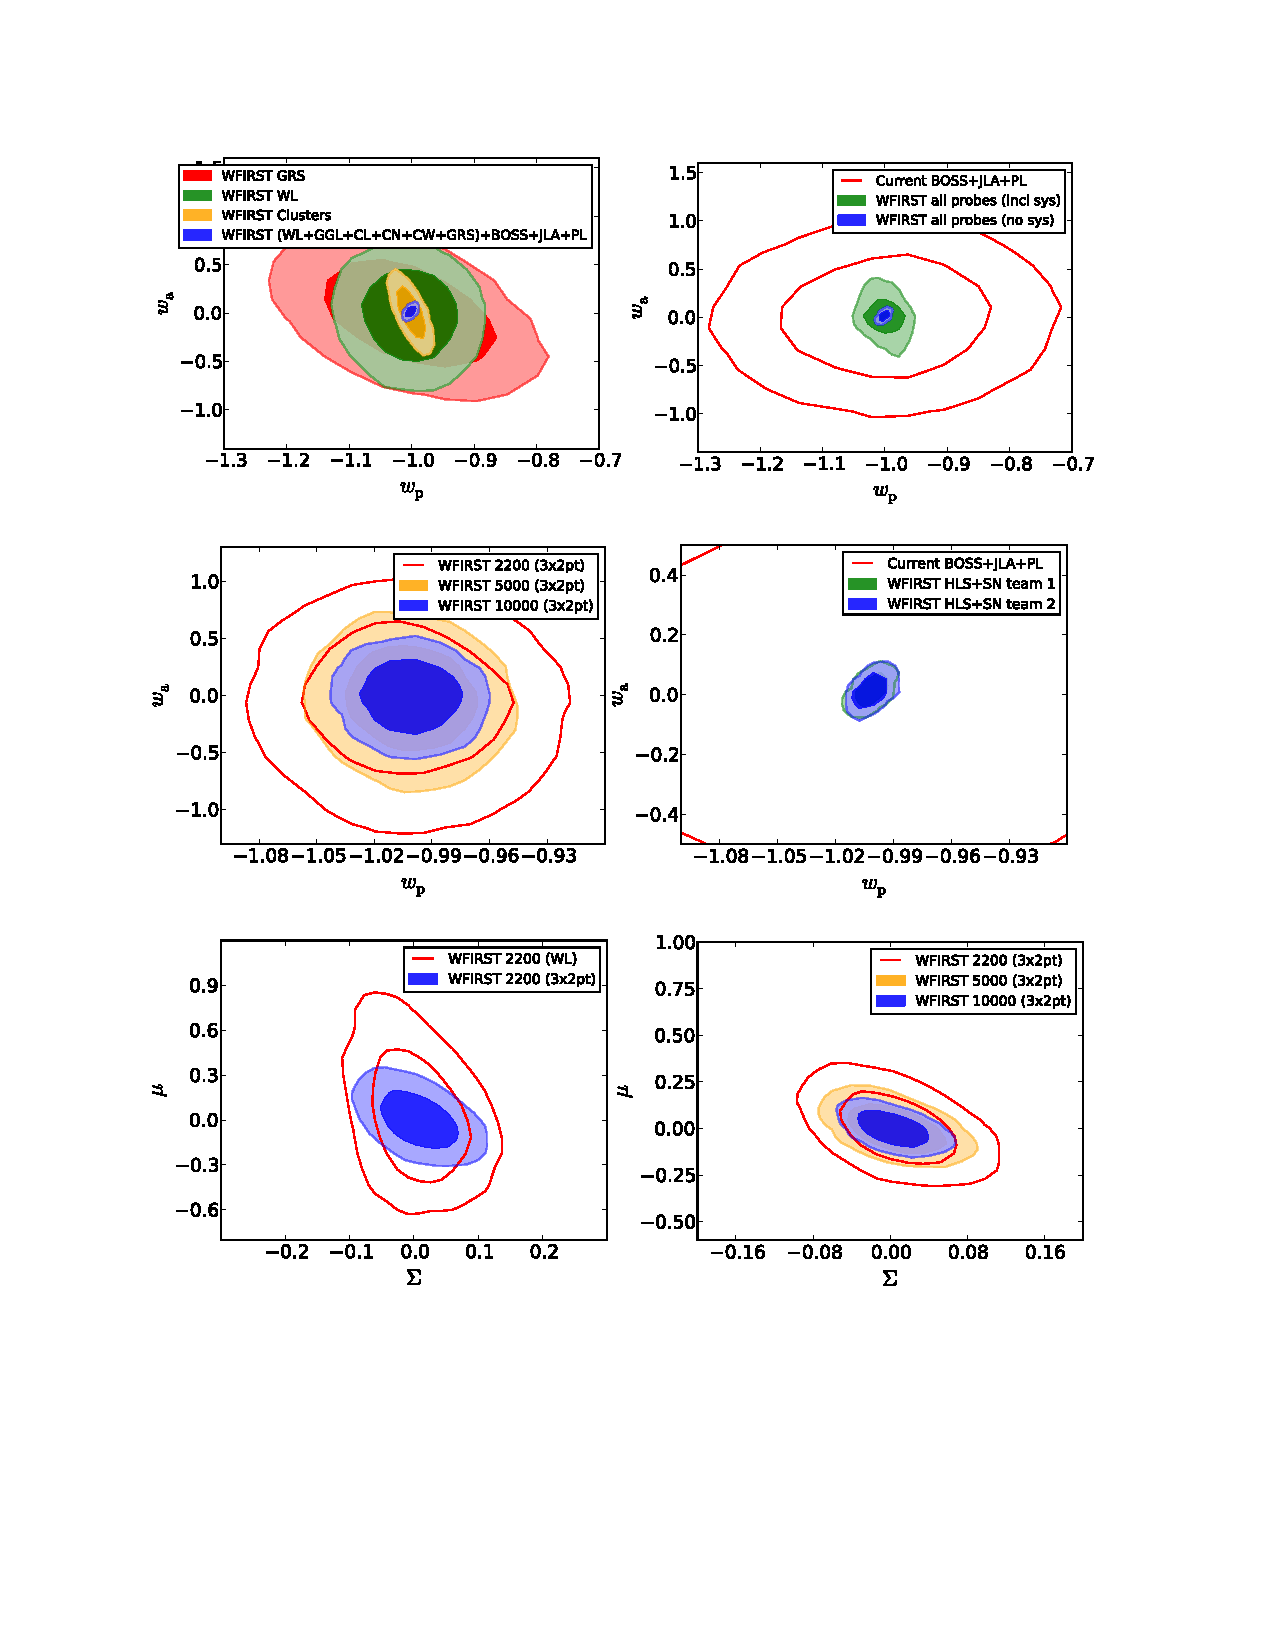
\includegraphics[width=15cm]{Plots/forecasts/multi}
\caption{WFIRST multi-probe studies, see text for details.}
         \label{fi:multi}
\end{figure*}

Developing a multi-probe cosmology analysis framework is challenging given that the analysis pipeline for individual probes are each under continuous development in order to meet the requirements of improving data quality. These efforts have historically been largely independent from each other; as a consequence, individual probe analyses utilize information from other probes to offset/calibrate systematics. 
For example, one of the most important astrophysical uncertainties for galaxy clustering is the relation of dark matter halos and luminous galaxies. The joint analysis of clustering and galaxy-galaxy lensing measurements removes uncertainties in this halo-galaxy connection when constraining cosmology. However, cosmic shear analyses use the same galaxy-galaxy lensing measurements to offset other systematic uncertainties (e.g., intrinsic galaxy alignment). This is only one example of many systematics mitigation conflicts that can occur when considering probes in isolation. A multi-probe analysis framework must account for these correlated systematic effects consistently across all probes; it cannot simply combine the optimal versions of individual analyses and it must include a global, well-designed systematics modeling and mitigation concept.

In this section we present a variety of simulated multi-probe WFIRST analyses; our results are summarized in Fig. \ref{fi:multi}. The upper left panel shows the constraining power of the individual survey elements (galaxy-redshift survey, weak lensing, galaxy clusters) in comparison to their combined constraining power plus galaxy-galaxy lensing, photometric galaxy clustering, and prior information from Planck, SN1a, BOSS. the likelihood analysis was carried out in a 7-dimensional cosmological parameter space, excluding any systematics. The right panel compares the aforementioned joint analysis (blue) with the current state of the art (red) and we show how the contours increase when including a realistic set of systematics in the analysis. These systematics include uncertainties arising from shear and photo-z calibration, cluster mass-observable relation, galaxy intrinsic alignment, and galaxy bias. Modeling and marginalizing over these systematics requires us to run a likelihood analysis in 54 dimensional parameter space; the details of our analysis are very similar to the LSST forecasts in \cite{Krause17}, but for WFIRST survey parameters (survey area, number density, and redshift distribution). 

The second row, left panel shows results from a simulated multi-probe analysis that can be extracted from the imaging survey only. The so-called 3x2pt analysis consists of second-order statistics from weak lensing, photometric galaxy clustering, and galaxy-galaxy lensing. We show the scaling of the error bars (statistics only, no systematics) when going from the nominal survey area to a 5000 and 10000 deg$^2$ survey.

The second row, right panel shows again our full multi-probe analysis including galaxy clusters and the spectroscopic survey component, i.e. BAO and RSD measurements, and we also include information from the 2 WFIRST supernovae teams. These team independently forecasted the WFIRST SN1a constraining power and are in excellent agreement. 

The lower row, left panel shows the constraining power of WFIRST weak lensing and 3x2pt for the nominal survey area on modified gravity parameters $\mu and \Sigma$ \citep[see e.g.,][for details]{jjk15, baa15}. The right panel shows the constraining power when increasing the survey area again to 5000 and 10000 deg$^2$. 

We emphasize that multi-probe studies are an area of active research and that the likelihood analyses presented here are the start of our intensive study to optimally combine WFIRST internal observables and also to study synergies of WFIRST and other, external data sets, in particular LSST. 






%\vspace{-0.15in}
%================================================
\section{Operations Model for the HLS and Evaluation of Trades}
%================================================
\label{sec:operation}

% C.H. Re-write of this section!

\begin{summary}
Co-I Hirata is leading the development of the HLS observing plan, extending his
previous tools used for the SDT. These tools incorporate observing constraints
in the chosen orbit, an exposure-by-exposure observing sequence optimized with
detailed model of overheads, and tiling/coverage maps including field
distortions and curved sky effects. These tools treat both imaging and
spectroscopy with unified functions and scripts, and are well suited to joint
survey optimization when both hardware parameters (e.g., reaction wheel
orientations) and the observing program (e.g., depth vs.\ area) are considered.
This effort is coordinated with the scheduling and Design Reference Mission (DRM)
Working Groups. We are both providing an example detailed plan for the HLS to
the DRM working group, and cross-checking the Project's spreadsheet-level survey
calculators against our simulations. The HLS observing plan is also being
transferred to the Calibration Working Group, since the HLS observing strategy
feeds directly into the issue of self-calibration.
\end{summary}

\subsection{Survey Optimization Principles}
%==========================================
%\Auth{David W, Chris, Olivier}
\label{sec:sur_opt}

%%%%The key constraint in survey optimization is the limited amount of observational time
%%%%available, since WFIRST is life-time limited and has multiple science focus areas.
%%%%For fixed instrumental capabilities and observing time, the most basic
%%%%decision to make about survey strategy is the trade between depth and total area.
%%%%In optimizing the WFIRST WL and BAO/RSD surveys, there are two key considerations:
%%%%(i) {\em precision} -- to maximize the DE science return of WFIRST, taking advantage of synergy with other surveys; and
%%%%(ii) {\em accuracy} -- tight control of systematic uncertainties, to ensure correct DE measurements.
The key constraint in survey optimization is the limited amount of observational time
available, since WFIRST is life-time limited and has multiple science focus areas.
For fixed instrumental capabilities and observing time, the primary
decisions on survey strategy are the trade between depth and total area, and
the balance between imaging and spectroscopy.
These decisions are driven by two major considerations:
\begin{itemize}
\item \emph{Pecision} -- to maximize the DE science return of WFIRST, taking advantage of synergies with other surveys; and
\item \emph{Accuracy} -- tight control of systematic uncertainties, to ensure correct DE measurements.
\end{itemize}
The combined expertise of our team in WL and GRS enables us to rapidly evaluate
these trades.

\paragraph{HLIS} The statistical power of a WL survey scales with the
total number of galaxy shape measurements, the product of the survey area and the effective surface density.
The SDT2015 report adopts an HLS imaging exposure time that yields roughly equal
contributions from read noise and sky noise in the most sensitive
filters, which approximately maximizes the total number of shape
measurements. This is a compromise between minimizing overheads and
read noise (which favors a ``deep'' mode), versus the shallow number
counts of resolved WL sources (shallower than $N\propto F^{-2}$, which
favors a ``wide'' mode). We re-examined the depth vs.\ area trade using
higher-fidelity tools (e.g., incorporation of shape measurement noise from realistic simulations, and updated
detector properties) and propagating the trades all the way to cosmological parameters
(using \CoLi).

\paragraph{HLSS} The depth vs.\ area trade for the GRS is driven by two
competing factors: for deep surveys, where the number density of galaxies $n$ is
large ($nP\gg 1$, where $P$ is the power spectrum at a given scale), the
information per unit area saturates; whereas for wide surveys, overheads reduce
inefficiency and galaxy shot noise inflates the statistical errors. In the SDT15
survey design, the GRS covers the same area as the HLS imaging survey ($\approx
2,200\deg^2$), to a $7\sigma$ limiting line flux of $\sim 10^{-16}
\erg\cm^{-2}\,{\rm s}^{-1}$ over most of the grism bandpass. This yields
approximately the largest number of galaxy redshifts for a fixed total observing
time. SDT15 found that doubling the survey area at fixed observing time (even
without additional imaging) {\it reduces} the precision of BAO measurements
because of the rapid increase in galaxy shot noise with decreasing spectroscopic
depth. However, this conclusion is sensitive to the luminosity function of
H$\alpha$ emitters at $z=1-2$, which remains uncertain
\cite{Mehta:2015,Pozzetti:2016}; Co-Is Teplitz and Wang lead our efforts to
reduce this uncertainty and feed the results into optimization of the GRS
(\S~\ref{sec:LF}).


\subsection{Snapshot of the HLS observing plan}
\label{ss:snapshot}

\begin{summaryii}
Our team provided a ``snapshot'' of the HLS observing sequence to the full FSWG
on April 19, 2017. This is by no means a final or even optimized version of the
HLS, but is a work in progress as a result of trades in Phase A, as well as the
recent decision to reduce the primary mission to 5 years.
\end{summaryii}

Major updates relative to the SDT plan have included:
\begin{itemize}
\item A Lissajous orbit around L2. This is presently a place-holder, as the exact orbit has not yet been selected (and would depend on the launch date), but it gives a possible sampling of Sun, Earth, and Moon constraints.
\item A rotated WFI (by 90$^\circ$ relative to the Cycle 6 design).
\item Recommended slew and settle times provided by the Project.
\item Faster detector readout (200 kHz instead of 100 kHz).
\item Changes to the exposure time and dithering strategy to accommodate a
5-year baseline mission (as is to be presented to the WIETR). Specifically, we
reduced exposure time to 140.2 s (imaging) and 297.0 s (spectroscopy); and
changed the dither pattern in J band. (We are working on checking this strategy
with image simulations, if it causes a problem we may have to revert.)
\item Implemented bright star avoidance (observations are skipped if there is an $H_{\rm AB}\le 3$ star within 6 arcmin of any SCA).
\end{itemize}
Known current issues with the snapshot plan include:
\begin{itemize}
\item
The SN and coronagraph programs in the code haven't been updated since the SDT
(except to cut the mission time by a factor of 5/6), even though they will
likely change significantly. As in the SDT report, the coronagraph has blocks of
time reserved. This will evolve in order to align the HLS plan with the other
groups, as well as any changes to the scheduling architecture that we are
directed to implement (e.g.\ block scheduling).
\item
We have begun putting the deep fields into this document, but right now they are
(i) not fully specified, (ii) the tiling is not optimized, and (iii) some roll
angles don't align with WFIRST constraints (hence didn't schedule). These issues
will be solved in the next snapshot.
\end{itemize}

We note that \emph{no policy decisions should be inferred from this sequence},
as these will come from a higher level.

The survey bounding box is 2,097 deg$^2$. The area covered with $\ge 3$ exposures
in every filter and the grism, including edge effects and holes around the
bright stars, is 1,947 deg$^2$. The time required for this version of the HLS is
394 days (imaging) + 215 days (spectroscopy).

The scheduling tools output a set of charts, included in this package:
\begin{itemize}
\item
Fig.~\ref{fig:observing_chart}: Graphical display of the 5-year observing sequence.
\item
Fig.~\ref{fig:hls_depth}: HLS distribution of number of exposures in each filter.
\item
Fig.~\ref{fig:hls_dust}: HLS distribution of dust column [$E(B-V)$ in magnitudes]. Cosmological forecasts are based on a dust column of $E(B-V)=0.035$ mag.
\item
Fig.~\ref{fig:hls_bright}: HLS distribution of zodiacal light (normalized to 1 at the ecliptic poles averaged over the year). Cosmological forecasts are based on a zodiacal brightness of 1.60 (except for 1.75 in the F184 filter, which is the least sensitive to zodiacal light and therefore was scheduled at inferior times of year).
\item
Fig.~\ref{fig:footprint}: The footprint of the HLS on the sky. This is an area of ongoing optimization, as we consider the needs of the deep fields, overlap with LSST, and the fraction of the survey footprint accessible from Northern observatories such as Subaru.
\end{itemize}

\begin{figure}
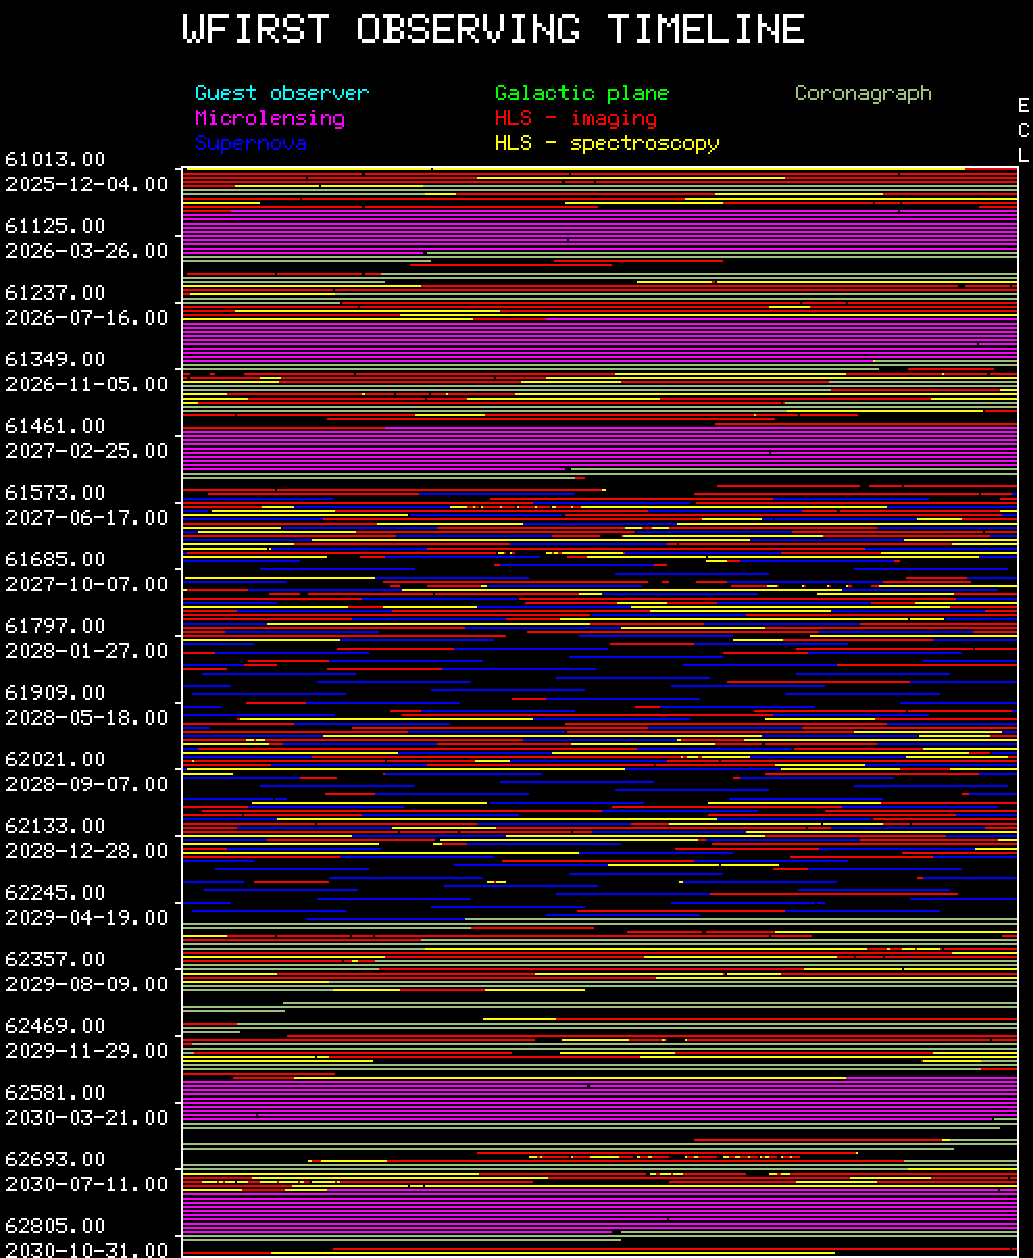
\includegraphics[height=8in]{Plots/observing_chart.pdf}
\caption{\label{fig:observing_chart}Observing timeline. Each row represents 7 days of observations, and is color-coded according to the observing program. Note the microlensing seasons (magenta), supernova survey (blue: $\sim$5-day cadence), and HLS (red+yellow). Blank areas are not allocated. Labels on the left-hand side are shown every 16 weeks.}
\end{figure}

\begin{figure}
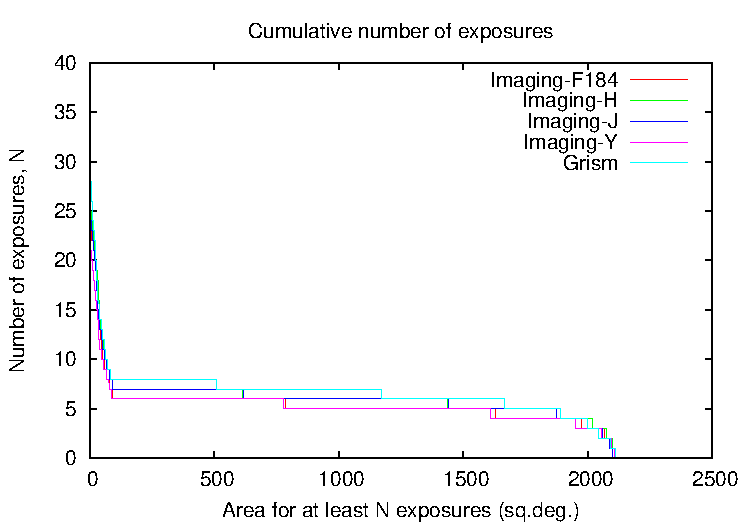
\includegraphics[width=5in]{Plots/hlsdepth.pdf}
\caption{\label{fig:hls_depth}The cumulative distribution of HLS exposure depths above a certain area. The pile-up with many exposures at small area is the result of the deep fields.}
\end{figure}

\begin{figure}
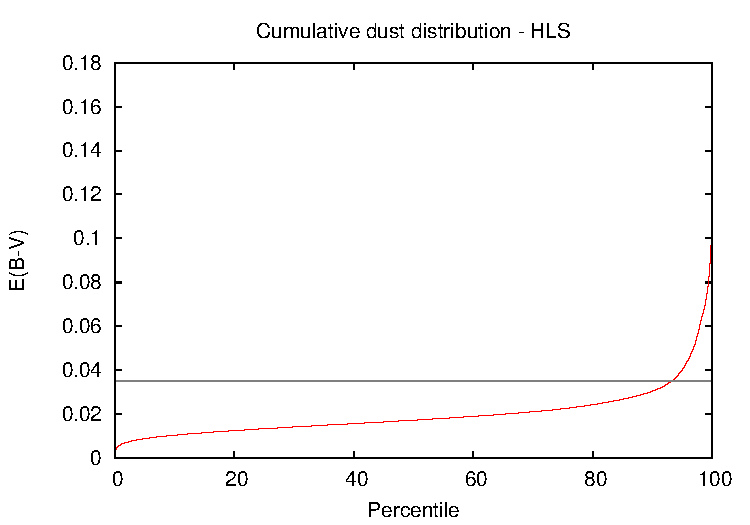
\includegraphics[width=5in]{Plots/hlsdust.pdf}
\caption{\label{fig:hls_dust}The cumulative distribution of Galactic dust in the HLS.}
\end{figure}

\begin{figure}
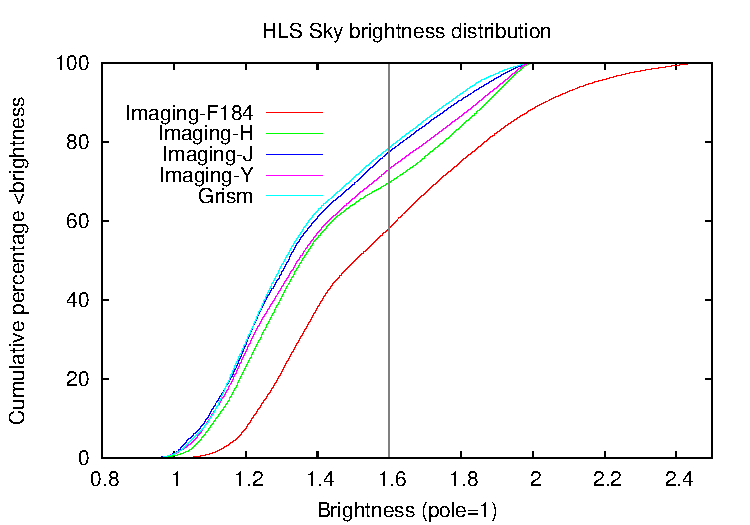
\includegraphics[width=5in]{Plots/hlsbright.pdf}
\caption{\label{fig:hls_bright}The cumulative distribution of zodiacal light in the HLS.}
\end{figure}

\begin{figure}
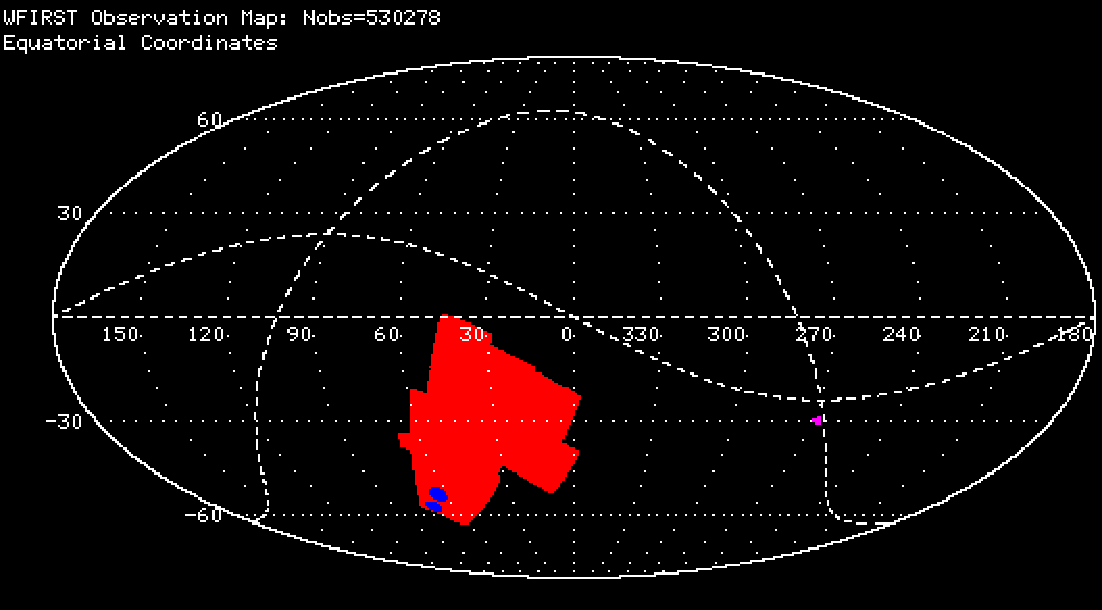
\includegraphics[width=6in]{Plots/sky-equ.pdf}
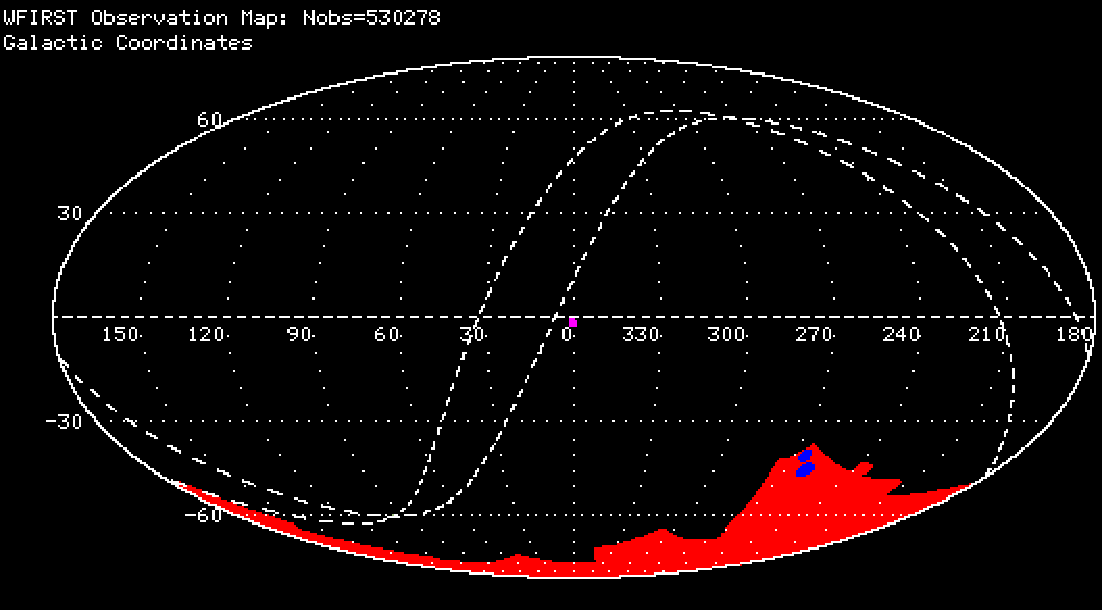
\includegraphics[width=6in]{Plots/sky-gal.pdf}
\caption{\label{fig:footprint}The footprint of the HLS (red) in Equatorial (top) and Galactic (bottom) coordinates.}
\end{figure}

\subsection{Further optimizations}

\begin{summaryii}
Our team plans to study further optimizations to the HLS -- including more
drastic changes such as multi-tiered surveys, or a significant re-balancing of
area vs.\ depth -- in Phase B. However, in preparation for SRR/MDR, our main
focus has been on demonstrating at least one survey configuration that meets
requirements, and the construction of tools that link the observing strategy to
calibration studies (\S\ref{sec:wl_calibration}) and image simulations (\S\ref{sec:hlis_image_sim}).
\end{summaryii}

The optimization of the WFIRST HLS will be tightly linked to operations simulations,
which inform the possible range of footprint area and location, depth in each filter (or grism), redundancy,
and temporal distribution of exposures. We propose a highly integrated approach, with the
operations simulations at the core, but with links to pixel-level simulations to assess required
redundancy, cosmological forecasting tools (\CoLi) to assess science reach, and comparison to the
observing regions of other surveys and telescopes to maximize synergies and meet requirements for
deep fields and photo-$z$ calibration.

% I hope this figure will just be combined with Fig 1.

%
%\setlength\intextsep{-2pt}
%%\begin{center}
%\begin{wrapfigure}{!ht}{0.45\textwidth}
% \begin{boxedminipage}{0.45\textwidth}
% \begin{center}
%\includegraphics[width=1.0\textwidth]{plots/like_DES_WFIRST_combi.eps}
% \end{center}
% \vspace{-1.25cm}
%\caption{{\footnotesize{ \Oli{Initial version for WFIRST vs DES} forecasts multi-probe science case. Probes included are cosmic shear, galaxy clustering, and galaxy-galaxy-lensing from WFIRST (black) in comparison to the Dark Energy Survey (green). The analysis includes BAO, SN1a and Planck information and accounts for galaxy bias, shear calibration, and photo-z errors (with different assumptions for the weak lensing and for the clustering sample). }}}
% \label{tab:milestones}
%\end{boxedminipage}
%\end{wrapfigure}
%% \end{center}
%\setlength\intextsep{0pt}

% \setlength\intextsep{-2pt}
% \begin{wrapfigure}{!ht}{0.75\textwidth}
%  \begin{boxedminipage}{0.75\textwidth}
%  \begin{center}
% \begin{figure*}
% \includegraphics[width=0.5\textwidth]{plots/WFIRST_multi.eps}
%% \caption{\textit{Placeholder plot for WFIRST forecasts multi-probe science case. Probes included are cosmic shear, galaxy clustering, and galaxy-galaxy-lensing, BAO with and without systematics (black and red contours, respectively). The systematics considered in this analysis are shear and photo-z uncertainties (which have different assumptions for the weak lensing and for the clustering sample), and linear galaxy bias. Blue contours include information from DES supernovae type 1a and green contours include an approximate version of Planck CMB temperature and polarization information.}}
%% {\bfseries C.H.: This belongs in another section.}
%%          \label{fi:WFIRST_multi1}
%% \end{figure*}

\subsection{Operations model (D7)}

Co-I Hirata will lead the development of the HLS observing plan,
extending his previous tools used for the SDT. These tools are already
highly advanced, incorporating observing constraints in the candidate
orbits (Geostationary Earth Orbit (GEO) or at the Lagrange point L2),
an exposure-by-exposure observing sequence optimized
with detailed model of overheads, and tiling/coverage maps including
field distortions and curved sky effects. These tools treat both imaging
and spectroscopy with unified functions and scripts, and are well suited to joint survey optimization when
both hardware parameters (e.g., reaction wheel orientations) and the
observing program (e.g., depth vs.\ area) are considered.
Hirata's operations tools were
used by the SDT for ``proof of principle'' studies, but we will now
extend them to (i) evaluate survey performance at intermediate stages
(e.g., what information is available after 1, 2, or 4 years); (ii)
include a pilot survey in the first few months of the mission to
validate HLS performance and make any ``early changes'' necessary;
(iii) include dedicated calibration observations as needed; and (iv)
export field overlap statistics as needed to assess internal calibration
strategies such as ``uber-calibration'' \cite{Padmanabhan2008}. This work will
be performed in consultation with other science groups on the FSWG and with
the WSC.

The SDT coverage maps included a study of the overlap with the LSST footprint,
but with our links to other projects we will understand the overlap with
the other cosmology surveys as well as the accessibility
of our fields from ground-based telescopes. This information, combined with the
community workshops (\S\ref{sec:engagement}), will be used to maximize synergies with
other facilities as well as ensure that potentially conflicting requirements (e.g.,
overlapping LSST photometry and photo-$z$ calibration including Northern telescopes
such as Subaru or Keck) can be met.

%\subsection{Synergies of WFIRST internal probes}
%=====================

%\subsection{Synergies of WFIRST and external data sets}
%=====================

\subsection{Survey Optimization (D10, D11)}
%=================================================
%\Auth{David W, Chris, Olivier}
\label{sec:sur_opt}

%%%%The key constraint in survey optimization is the limited amount of observational time
%%%%available, since WFIRST is life-time limited and has multiple science focus areas.
%%%%For fixed instrumental capabilities and observing time, the most basic
%%%%decision to make about survey strategy is the trade between depth and total area.
%%%%In optimizing the WFIRST WL and BAO/RSD surveys, there are two key considerations:
%%%%(i) {\em precision} -- to maximize the DE science return of WFIRST, taking advantage of synergy with other surveys; and
%%%%(ii) {\em accuracy} -- tight control of systematic uncertainties, to ensure correct DE measurements.
The key constraint in survey optimization is the limited amount of observational time
available, since WFIRST is life-time limited and has multiple science focus areas.
For fixed instrumental capabilities and observing time, the primary
decisions on survey strategy are the trade between depth and total area, and
the balance between imaging and spectroscopy.
These decisions are driven by two major considerations:
(i) {\em precision} -- to maximize the DE science return of WFIRST, taking advantage of synergies with other surveys; and
(ii) {\em accuracy} -- tight control of systematic uncertainties, to ensure correct DE measurements.
The combined expertise of our team in WL and GRS will enable us to rapidly evaluate
these trades, informed by results from previous and concurrent surveys such as
DES/DESI/Euclid. Furthermore, we plan on developing pipelines to
rapidly analyse ``pilot'' data from WFIRST to quantify the telescope
and instrument performance, as well as developing well defined metrics to guide the survey trades.

\subs{WL Survey.} The statistical power of a WL survey scales with the
total number of galaxy shape measurements, the product of the survey area and the effective surface density.
The SDT2015 report adopts an HLS imaging exposure time that yields roughly equal
contributions from read noise and sky noise in the most sensitive
filters, which approximately maximizes the total number of shape
measurements. This is a compromise between minimizing overheads and
read noise (which favors a ``deep'' mode), versus the shallow number
counts of resolved WL sources (shallower than $N\propto F^{-2}$, which
favors a ``wide'' mode). However, we will re-examine the depth vs.\ area trade using
higher-fidelity tools (e.g., incorporation of shape measurement noise from realistic simulations, and updated
detector properties) and propagating the trades all the way to cosmological parameters
(using \CoLi).
We will also investigate the performance of hybrid strategies in
which a four-filter survey over part of the HLS area is combined
with a one- or two-filter survey over a larger area.  This approach
would yield more independent shape measurements at the cost of
greater \photoz\ uncertainties and complicating cross-checks of systematics,
so assessing it requires attention to the entire path from data
to scientific conclusions, including the impacts
on scientific investigations outside of dark energy and cosmological
parameters.

\subs{GRS Survey.} The depth vs.\ area trade for the GRS is driven
by two competing factors: for deep
surveys, where the number density of galaxies $n$ is large ($nP\gg 1$, where $P$ is the power spectrum at
a given scale), the information per unit area saturates; whereas for wide surveys, overheads
reduce inefficiency and galaxy shot noise inflates the statistical errors.
In the SDT15 survey design,
the GRS covers the same area as the HLS imaging survey
($\approx 2,200\deg^2$), to a
$7\sigma$ limiting line flux of $\sim 10^{-16} \erg\cm^{-2}\,{\rm s}^{-1}$
over most of the grism bandpass.
This yields approximately the largest number of galaxy
redshifts for a fixed total observing time.
SDT15 found that doubling the survey area at fixed observing time (even without
additional imaging) {\it reduces} the precision of BAO measurements
because of the rapid increase in galaxy shot noise with decreasing
spectroscopic depth.
However, this conclusion is sensitive to the luminosity function of
H$\alpha$ emitters at $z=1-2$, which remains uncertain \cite{Mehta2015,Pozzetti2015};
Co-Is Teplitz and Wang will lead our efforts to reduce this uncertainty
and feed the results into optimization of the GRS.

We will study the link between the observing strategy and systematic error
validation.  For example, pixel-level simulations will predict the variation of
galaxy density with respect to the diversity of roll angles, use of subsets of
the exposures in the data reduction, etc.; our team has extensive experience
with the measurement of such dependences in imaging surveys (Co-Is Ho, Hirata,
Padmanabhan)
and will extend this to the GRS. The hardest part of the GRS error
validation will be galaxy biasing: while it is possible to ``test'' bias models
against a range of simulations with plausible prescriptions for galaxy
placements (HODs, SAMs, etc.), we will ultimately need to validate galaxy
biasing models against the data itself. The most promising avenues are
higher-order statistics (such as 3-point correlations)
and the consistency of results obtained from subsets of the galaxy sample
(e.g., split by magnitude or color).
Both of these demand larger $nP$ and drive
the survey deeper than the power spectrum measurement.
We will develop the tools to assess the precision of these
validation tests and will incorporate them into the survey optimization.

A key consideration in the depth vs.\ area trade is the relation to the Euclid
and DESI redshift surveys; the optimization of WFIRST GRS should avoid portions
of this space that will already be well-explored by these other projects and
focus on the unique capabilities provided by a large telescope in the
low-background space environment.

%Given the assumptions about instrument
%performance and empirical model of the H$\alpha$ luminosity function
%adopted in SDT2015, this exposure time is approximately the one that
%yields the largest number of galaxy redshifts for a fixed total
%In the SDT2015
%survey design, the GRS covers the same area as the HLS imaging survey
%($\approx 2200\deg^2$), and the exposure time of 347 sec yields a
%$7\sigma$ limiting line flux of $\approx 10^{-16} \erg\cm^{-2}\sec^{-1}$
%over most of the grism bandpass.
%
%observing time (0.68 years in SDT2015).
%However, the statistical power
%of a redshift survey does not scale trivially with the number of galaxies,
%and the optimal choice can be quite different for different applications.
%
%The variance in a measurement of the galaxy power spectrum at
%wavenumber $k$ scales inversely with the effective comoving survey volume
%\begin{equation}
%V_{\rm eff}(k) = \int d^3r  [1+nP(k)]^{-1}~,
%\end{equation}
%where $n$ is the galaxy space density.  {\bf Agreed?}
%The optimal tradeoff between depth and area typically occurs
%for $nP = 1-2$; at higher $nP$ it is better to expand the survey
%area to increase volume, while at lower $nP$ it is better to
%go deeper to reduce shot noise.
%SDT2015 forecasts $nP \approx 2-3$ (depending on redshift)
%at the scale $k=0.2\mhmpcinv$
%that is relevant for BAO precision, which suggests that the BAO
%precision could be improved moderately by decreasing the exposure
%time and increasing the survey area; because the survey depth is
%already on the exponential tail of the H$\alpha$ luminosity function,
%the space density drops rapidly with increasing flux limit.
%However, even for the relatively simple case of BAO, optimization
%depends sensitively on instrument characteristics (detector read noise,
%grism throughput, etc.), on the imperfectly known H$\alpha$ and [OIII]
%luminosity functions, on the performance of reconstruction methods,
%and on details of data reduction and incompleteness corrections.
%For example, the methods recently proposed by \cite{suchyta2015}
%could allow effective use of emission line sources down to a $\sim 5\sigma$
%limit, instead of the conservative $7\sigma$ detection threshold assumed by
%SDT2015, and this would significantly shift the optimal exposure time.
%For RSD the optimization depends additionally on the accuracy of theoretical
%techniques to model non-linear galaxy clustering, since this determines
%the maximum wavenumber at which power spectrum measurements are cosmologically
%useful.  We also hope that the methodology investigations described
%above will provide powerful new routes to cosmological parameter constraints
%from higher order clustering measurements, which are more sensitive to
%shot noise.  Relative to power spectrum analyses, these methods likely
%favor a denser survey with higher $nP$, but survey optimization for
%such analyses is largely uncharted territory.

\subs{WFIRST HLS Survey.}  Optimization of the WFIRST HLS requires the end-to-end approach
outlined in this proposal, considering everything from the read noise
of the detectors and contamination of redshift catalogs to the
theoretical modeling systematics for higher order clustering statistics.
It also requires joint consideration of the imaging and spectroscopic
surveys:
multi-filter photometry (as planned in SDT2015) is required to suppress
contaminants in the GRS \cite{Pullen2015}.
We will provide, in addition to our own recommendations,
publicly available tools that can be used by future science teams,
the WFIRST Project, and the community at large to evaluate a variety
of HLS strategies, including changes to the balance between imaging
and spectroscopy.  These tools will enable us and others to incorporate
updated information about instrument and software performance,
empirical data on the galaxy population, progress in modeling techniques,
the expected contributions of other projects like DESI, LSST, and Euclid,
and changes in the experimental dark energy landscape that highlight
the importance of particular classes of measurements.

%}


%====================================================
\section{Community Engagement and External Data-sets}
%====================================================
\label{sec:engagement}
%
% ** SECTION 8 **
%

\begin{summary}
The coming decade will be an exciting time for cosmology. Before WFIRST launch,
major cosmological imaging surveys (KiDS, HSC, DES) and the DESI and PFS
spectroscopic surveys will significantly advance our current understanding.
WFIRST, Euclid and LSST  will then go further and survey the sky at optical and
infrared wavelengths, the  James Webb Space Telescope (JWST) and the Extremely
Large Telescopes (ELTs) will make very deep maps of the sky; eROSITA will survey
the X-ray sky; CMB-S4 will make a deep map of the millimeter sky; and the
Canadian Hydrogen Intensity Mapping Experiment (CHIME) and other radio surveys
will map the large-scale distribution of H$\,${\sc i}. One goal of our SIT is to
determine the analysis infrastructure and observations needed to achieve the
full potential of WFIRST in combination with these  surveys. This is best done
through a broad community effort that brings together scientists from these
complementary projects. For this purpose, we organized a first community
workshop focused on enabling the cosmological scientific synergies between
WFIRST and LSST.
\end{summary}

Our SIT naturally brings close connections to most of the
major current or planned cosmological experiments that will provide
the context for the WFIRST dark energy program. This includes the WMAP and Planck CMB missions,
the Sloan Digital Sky Survey (SDSS), the Baryon Oscillation Spectroscopic Survey (BOSS), the Dark Energy Survey (DES),
the Subaru Hyper Suprime-Cam (HSC) and Prime Focus Spectrograph (PFS)
projects, the Dark Energy Spectroscopic Instrument (DESI), the
Euclid mission and the Large Synoptic Survey Telescope (LSST) Dark
Energy Science Collaboration (DESC).

% Our team of U.S. and international collaborators brings extensive expertise in detector
%characterization, cosmological simulations, detailed simulations of
%observational data sets, and the theoretical modeling and cosmological
%interpretation of weak lensing and galaxy clustering data.
%Notably, members of our team are responsible for nearly all of the tables
%and figures in \S\S\ 2.2.3-2.2.5 of the SDT15 report, describing the
%HLS dark energy program.  We therefore have an unparalleled understanding
%of the current design of WFIRST-AFTA and of the
%challenges ahead in achieving its science goals.

%Our SIT team is well-placed to do this, through team members' significant roles in a number of these projects and ties to the other major surveys.

%Our team will explore ways of maximizing the science return from these combined data sets. Our team members are playing significant roles in a number of these projects and have good ties to the other major surveys.

We also started to actively engage the community to identify and pursue the key areas
where WFIRST and the concurrent projects will provide new opportunities to
mitigate systematics and enhance the combined cosmological science return. We
started a series of open community workshops to incorporate the interplay
between major planned surveys and WFIRST into the WFIRST strategy, to identify:
(i) pre-launch observations, (ii) how these external data sets affect the WFIRST
observing strategy (e.g., deep fields) and the instrument, and (iii) the
software needed (to be built post-CDR) for combining these data sets.

\paragraph*{First Community Workshop} The first of this meeting happened in
Pasadena in September 2016. It was focused on the synergies between the WFIRST
HLS Cosmology SIT and LSST Dark Energy Science Collaboration (DESC), both at the
science level but also at the implementation level. The meeting was co-organized
by Rachel Bean, Olivier Dor\'e, Steve Kahn and Jason Rhodes and was attended by
about 60 scientists from the two collaborations. The slides are available
\href{https://conference.ipac.caltech.edu/wfirst_lsst/}{here} and pictures can
be seen in Figure~\ref{fig:pic_workshop}. The conclusion of the lively and
productive workshop will be summarized in a white paper to be written shortly.

\begin{figure}
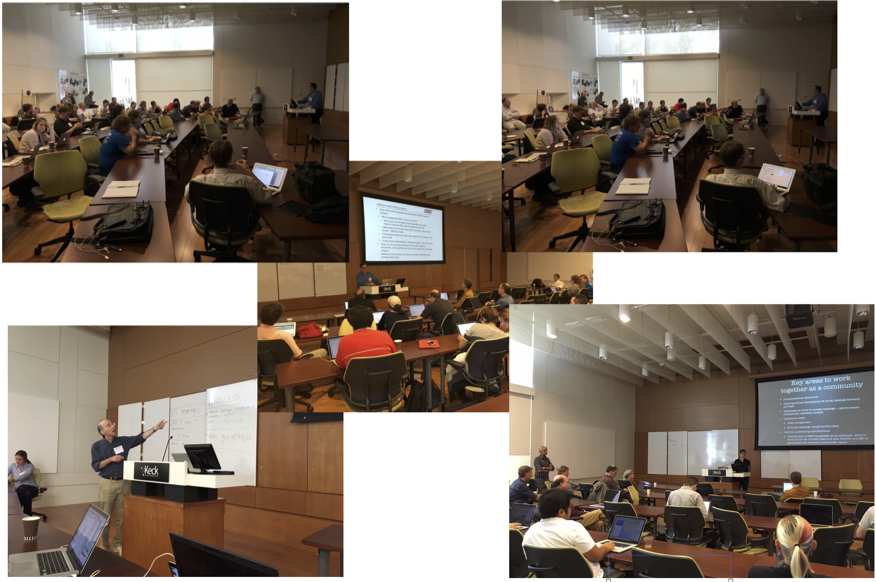
\includegraphics[width=\textwidth,angle=0]{Plots/pic_workshop.png}
\caption{\label{fig:pic_workshop}Pictures taken during the Pasadena WFIRST SIT - LSST DESC workshop on September 2016.}
\end{figure}

\paragraph*{Premise} The workshop was built on the premise that when considering
joint science return from LSST and WFIRST, \emph{the whole is greater than the
sum of the parts}, as already articulated in \citet{Jain:2015cpa}. In the
conclusion of the Jain et al. community white paper, it was articulated that the
scientific opportunity offered by the combination of data from LSST and WFIRST
(and Euclid) goes well beyond the science enabled by any one of the data sets
alone. The range in wavelength, angular resolution and redshift coverage that
these missions jointly span is remarkable. With major investments in LSST and
WFIRST (and partnership with ESA in Euclid), the US has an outstanding
scientific opportunity to carry out a combined analysis of these data sets. It
is imperative for us to seize it and, together with our European colleagues,
prepare for the defining cosmological pursuit of the 21st century.

As illustrated already in \S~\ref{sec:forecast}, the coming decade will be the
era of multi-probes/multi-survey science. The richer insights will come from
combining multiple probes (WL, GRS, GC) \emph{reliably}. If done properly,
multiple survey joint analysis will enable new calibration schemes (photo-$z$,
intrinsic alignment models, etc.) and new control of systematics (PSF effects,
contaminant control such as stars or interlopers).

\paragraph*{Joint Analysis} The main argument for conducting a single,
high-quality reference co-analysis exercise and carefully documenting the
results is the complexity and subtlety of systematics that define this
co-analysis. Falling back on many small efforts by different teams in selected
fields and for narrow goals will be inefficient, leading to significant
duplication of effort.  For much of the science, we will need to combine the
photometry across multiple wavelengths with varying spectral and spatial
resolution – a technical challenge. The joint analysis can be carried out in
ways that have different computational demands. The most technically demanding
joint analysis is to work with pixel level data of the entire area of overlap
between the surveys. Many of the goals of a joint analysis require such a
pixel-level analysis. If pixel-level joint analysis is not feasible,
catalog-level analysis can still be beneficial, say to obtain calibrations of
the lensing shear or the redshift distribution of galaxies. Hybrid efforts are
also potentially useful, for example using catalog level information from space
for deblending LSST galaxies, or using only a mutually agreed subset of the data
for calibration purposes. However the full benefits of jointly analyzing any two
of the surveys can be reaped only through pixel-level analysis \citep{Jain:2015cpa}.

\paragraph*{Possible Implementation} In the workshop, possible algorithmic
implementation of a joint analysis pipeline were discussed independently by
Peter Melchior and Michael Schneider. \citet{Melchior:2016asy} motivated the
need for complex galaxy morphology models and developed the relevant statistical
framework. For them, complex models become the norm. They are more flexible and properly
behaved. WFIRST benefits from LSST through color-morphology priors. LSST
benefits from sharp likelihood peaks in WFIRST bands. LSST benefits from WFIRST
through superior resolution. \citet{Schneider:2014rha} have developed a probabilistic
image reduction pipeline (forward modeling) motivated by challenges in
multi-epoch/multi-telescope combinations. They demonstrated improved shear
measurements for LSST using the HST Frontier field as a proxy for WFIRST.

\paragraph*{Enabling Synergies} It was recognized in the context of photo-$z$ for example, that
cooperation already exist to maximize utility and minimize duplication in
spectroscopic calibration samples. Capak and collaborators are building a public
calibration catalog for WFIRST and LSST \citep{Masters2017}. Also, relevant information for deep
surveys synchronization, is also discussed in this context and others (SNe,
shape calibration, grism calibration, guest observations). The detailed requirements for LSST + WFIRST photo-$z$ performance are however still to be articulated.

\paragraph*{Computing Needs} Large computing efforts are under way in LSST
(DESC) with multiple planned data challenges. Resources available for the scale
of simulations required (with possible exception of hydrodynamical simulations)
are secured. However, ressources needed for sharing simulations (e.g. Millennium
DB) and mock catalogs are required. They have historically greatly 
expanded the
use of simulations in a broad range of applications. A 100 TB to 1 PB scale
infrastructure simply does not exist and data transfer will be a challenge (10
days for 100 TB at 1 Gb). There is great opportunity for future collaborations
(e.g., joint mock catalogs) and investments. Opportunity for collaborations and
investments. As we will discuss in \S\ref{sec:tacs}, members of our team are leading and participating in a Tri-Agency Cosmological Simulations (TACS) dedicated to this issue.

\paragraph*{Ressources} As already discussed in \citet{Jain:2015cpa}, the resources required to achieve this additional
science are outside of what is currently budgeted for LSST by NSF and DOE, and
for WFIRST (or Euclid) by NASA. Funding for this science would most naturally
emerge from coordination among all agencies involved, and would be closely
orchestrated scientifically and programmatically to optimize science returns. A
possible model would be to identify members of the science teams of each project
who would work together on the joint analysis. The analysis team would ideally
be coupled with an experienced science center acting as a focal point for the
implementation, and simultaneously preparing the public release and documentation for broadest access by the community.

\paragraph*{Future Workshop} The second in our series of SIT community workshop
will happen in the fall 2017 in Pasadena, synchronized with a FSWG, and will
identify (and discuss the enabling of) scientific synergies between the HLS and
other major surveys across all wavelengths.


%======================================================
%\section{Future Workplan \Oli{Olivier, all, 5 pages}}
%======================================================
%\label{sec:workplan}
%%
% ** SECTION 8 **
%

% \setlength\intextsep{-2pt}
% \begin{wrapfigure}{r}{0.5\textwidth}
%  \begin{boxedminipage}{0.5\textwidth}
%  \begin{center}
% \epsfig{file=Plots/team_flow_v1.pdf,angle=0,width=0.99\textwidth}
%  \end{center}
%  \vspace{-0.5cm}
%  \caption{{\footnotesize {Team members commitment to the
%        deliverables listed in \S~\ref{sec:deliverables}. The task lead
%        is in red but for some tasks, we identify separate leaders for
%        WL with a green diamond, GRS with a blue star, and Clusters
%        with a purple triangle.  For D2, we expect Co-I Eifler to
%        take over from PI Dor\'e as overall lead following FY16.}}}
%  \label{tab:flow}
%  \end{boxedminipage}
%  \end{wrapfigure}
%  \setlength\intextsep{0pt}

\subs{Team Management.} We have structured our team to 
cover all the areas of expertise required for
the proposed work, and to maximize the synergies between WFIRST
and the cosmology community.
Scientific decisions including the allocation of
funds will be made by the PI in consultation with a Steering 
Committee consisting of the PI, the two topic leads (Hirata and Wang),
the topic sub-lead Weinberg plus Spergel, who have extensive organizational experience
through WMAP, ACT, SDSS, National Research Council (NRC) and NASA
committees, and other activities. While the PI will have final authority on these decisions,
this Committee has the mission experience and breadth of knowledge
needed to advise the PI. Monthly Steering 
Committee telecons will review the budget and priorities so that our
effort
remains focused on the scientific success of WFIRST.
Each topic lead will report to the PI on a monthly basis, to facilitate monitoring
of all team work, enable advice on budget priorities, and ensure a
regular review of work effort. The PI will ensure proper
communication with the WFIRST program office and will maximize
collaborations with other WFIRST SITs. For
example, we anticipate jointly developing and sharing low-level image
simulation tools with SN-focused SITs. Topic leads will closely
monitor the progress of the technical tasks (listed in
\S\S~\ref{sec:deliverables},\ref{sec:wl_gal-clusters},\ref{sec:gc}) in
association with the deliverables and will adjust the scope of the
work according to developments in the project and in the field.

\subs{Risk Management.} Inefficient collaboration/coordination presents
the most significant risk for accomplishing our program. Within our
 SIT, this is mitigated partly by most Co-Is having experience
working together in existing (or past) projects. The PI will
coordinate the team's effort, and ensure it is well-integrated into
and aligned with the broader WFIRST effort. The PI will lead the following: 
%  to ensure a productive, harmonious, and coordinated collaboration. (1) the PI will 
(i)  Monthly telecons with the Steering Committee, to optimize the team effort; (ii) 
Regular telecons with all team members, with status updates
from the deliverables leads (Fig.~\ref{tab:flow}) so that progress, issues, and
solutions are broadly visible across the team. (iii) Yearly face-to-face
meetings and more focused working meetings will be added as
needed (the associated travel costs have been 
budgeted). Monthly, the Steering Committee will evaluate progress
reports and redistribute responsibilities within the team if 
necessary. Finally, team members will present %(in person or remotely) 
recent progress, results, and goals for the upcoming year to
an external review panel at this annual meeting. This will also serve as a NASA management
review with representatives of NASA HQ and the JPL WFIRST Project
Office invited to attend. This follows the successful model used by
the US Planck and US Euclid teams with which the PI and many Co-Is have
experience. The PI will also set-up wikis and repositories for efficient
sharing and discussion of software, documents, plans, progress and
issues. We plan to share with the community the software developed for
this program. Key results will be published in peer review papers.

\subs{Program Milestones.} In Fig.~\ref{tab:milestones_mgt} we outline milestones for
our effort in conjunction with the
\setlength\intextsep{-2pt}
%\begin{center}
\begin{wrapfigure}{r}{0.75\textwidth}
 \begin{boxedminipage}{0.75\textwidth}
 \begin{center}
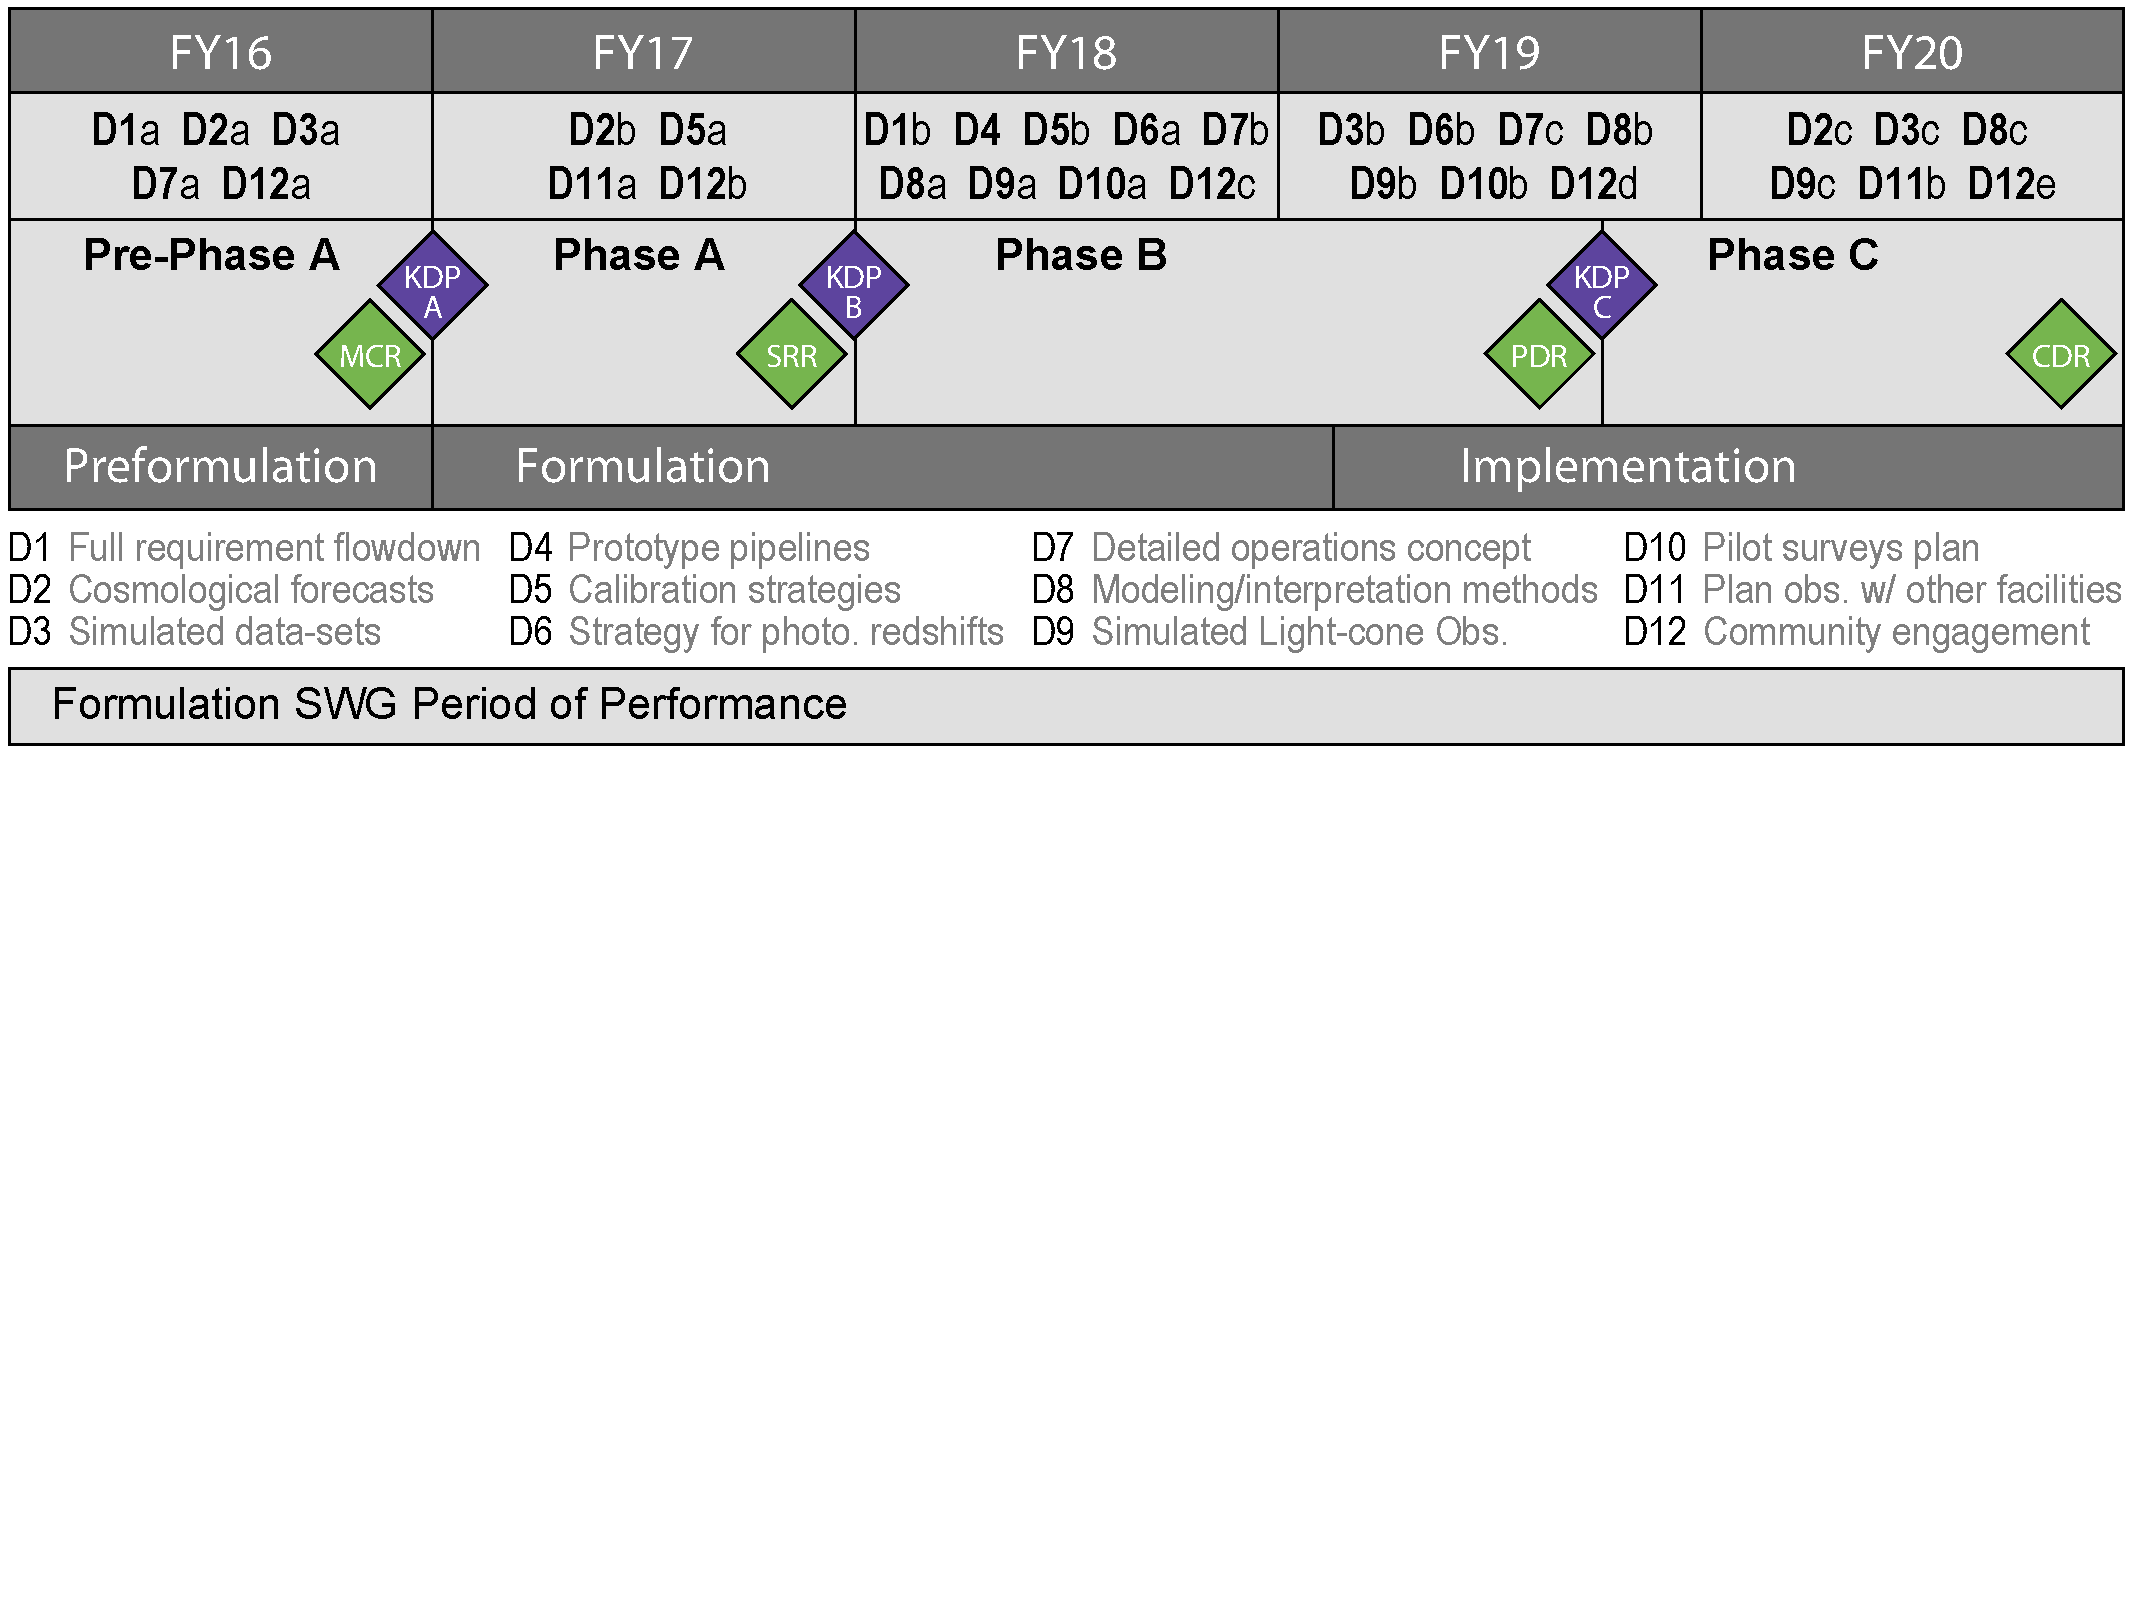
\epsfig{file=Plots/wfirst_milestones_v2.pdf,angle=0,width=0.99\textwidth}
 \end{center}
 \vspace{-0.5cm}
 \caption{{\footnotesize Our deliverable schedule in concordance with the
       WFIRST project timeline as displayed in the WFIRST SIT call \S
       3.2. Deliverables that are made in multiple stages are labeled
       (a, b and c) and appear in multiple years.}}
 \label{tab:milestones_mgt}
 \end{boxedminipage}
 \end{wrapfigure}
%\end{center}
\setlength\intextsep{0pt}
project timeline.

\subs{Postdocs and Students.}  The largest component of our budget is support for postdoctoral researchers
who will work under the supervision of the PI and Co-Is to carry out the
many calculations, simulations, and tests needed to accomplish our
tasks.  Our budget incorporates an initial plan for which postdocs will
be located at which institutions in which years to work on which tasks.

However, the optimal division of labor may shift over time, and the
Steering Committee will consider reallocations of work annually
based on internal proposals from team members.  Where appropriate,
we will consider raising collaborators to funded Co-Is, with NASA approval,
if they are best positioned to carry out particular tasks.
Many of the methodology development efforts, and some of the
technical tasks, are well suited to graduate students, supported
by other sources or by this Investigation if their work
clearly falls within its scope.  In addition to accomplishing the
work of this proposal, the involvement of many postdocs and students
will build a cadre of young researchers who are ideally positioned
to exploit the scientific opportunities of WFIRST.

\subs{A Unified Team.} As is evident from our previous discussion, jointly addressing the
weak lensing and redshift-space clustering elements of the WFIRST
dark energy program leads to an ambitious task list that offers critical
advantages relative to studying them separately.  First is the effective use of expertise; many members of
our team have expertise in both of these program elements and will
contribute to both during the course of this investigation. Second is
the commonality of the hardware; HLS Imaging and Spectroscopy use the
same telescope, detectors, and data systems, and it makes sense to develop associated requirements
through joint consideration of the two surveys.
Third is the need to develop a unified operations concept for these
two interleaved surveys; in overall footprint and in details of
dither patterns and roll angles, choices made for one survey affect
the performance of the other.

Finally, a joint investigation allows us to take a broad perspective
on the WFIRST dark energy program, including a common forecasting
framework that can account for complementary information and the
ability of one survey to mitigate systematics in the other,
common sets of cosmological simulations and models of galaxy bias
that are relevant to both topics, and investigation of trades
between HLS Imaging and Spectroscopy.  We have carefully
constructed a team capable of addressing all of the essential tasks for elements A and C of the WFIRST SIT NRA, and
we have requested resources that will enable us to accomplish this work.
If NASA decides to select additional teams in these areas we will be glad to collaborate with them. 
As emphasized in \S\ref{sec:engagement}, WFIRST is a national and international resource, and
it is valuable to engage as much of the astronomical community
as possible in its formulation.  



%===========================================================
\section{Other Science Investigation Team Contributions to WFIRST Mission}
%===========================================================
\label{sec:other_contributions}
% Other contributions


\begin{summary}[SUMMARY POINTS]
Our SIT engaged in multiple other activities supporting the WFIRST mission and the Project Office not discussed above. We summarize them here.
\begin{enumerate}
\item Our SIT actively participated to two workshops dedicated to the WFI;
\item Our SIT contributed to evaluate the Supernova Program;
\item Our SIT partially supported 15 post-doctoral researchers and one graduate student;
\item Our SIT published 10 scientific papers supporting our studies or extending the scientific case of WFIRST;
\item SIT team members are leading the Tri-agency Cosmological Simulation Task Force (TACS);
\item Our team delivered to the community several high-value products and softwares.
%--------------------------------------------------------------------------
\end{enumerate}
\end{summary}


\subsection{\emph{Princeton Meetings} Participation}
%---------------------------------------------------------------

In addition to the active participation by the SIT leads to the 4 FSWG meetings that happened this year, team members participated to two focused so-called \emph{Princeton Meetings} meetings organized by Prof. Spergel in Princeton University and at the newly established Flatiron Institute in  New York, NY. These two meetings were focused respectively on planning the data processing need of the WFI given our collective experience with large astronomical datasets data processing, and ancillary science enabled by the HLS. Team members Lupton, Mandelbaum, Samushia, van der Linden represented our SIT at this meeting and presented their thoughts on these topics.

\subsection{Contributions to Evaluation of the WFIRST Supernova Program}
%------------------------------------------------------------------------

In addition to our work on the HLS cosmology surveys,
team members Olivier Dor\'e, Chris Hirata, David Spergel,
and David Weinberg all contributed to evaluating strategies and
requirements for the WFIRST supernova program, providing a
sounding board for the two supernova SITs and synthesizing
information for project management.  Some of these contributions
took place in sessions of the WFIRST FSWG meetings and some
of it in telecons and email exchanges with members of the
supernova teams.  Weinberg wrote an extensive referee report
for the Hounsell et al.\ paper (from the supernova SIT led by
Ryan Foley) on WFIRST supernova strategies.  Most importantly,
all four investigators participated in the ``supernova summit''
held at KIPAC in March 2017, reading background material from
the teams, participating in a day of presentations and discussions,
and writing a report for project management and the supernova SITs.


\subsection{Supported Postdoctoral Researchers and Graduate Students}
%--------------------------------------------------------------------

Our team has been very proactive at leveraging our collective involvement in other on-going large scale observational efforts such as the Dark Energy Survey (DES), the SUBARU Hyper-Suprime Cam (HSC) survey, but also the joint ESA/NASA Euclid mission and the Large Synoptic Survey Telescope Dark Energy Science Collaboration (LSST DESC) to create joint appointments and assemble a team of very strong postdoctoral researchers. In particular, the following researchers joined our team and are partially supported by out SIT:
\begin{itemize}
\item Ivano Baronchelli (Caltech/IPAC), working with Harry Teplitz on updating measurements of the H$\alpha$ luminosity function using HST data;
\item Ami Choi (OSU), working with Chris Hirata and David Weinberg on image simulations for the WL analysis;
\item Shoubaneh Hemmati (IPAC/Caltech), working with Peter Capak on defining the photometric redshift requirements of the WFIRST WL investigation;
\item Albert Izard (JPL), working with Alina Kiessling on cosmological simulations and the requirements driven by the need to accurately compute covariance matrices;
\item Niall MacCrann (OSU), working with Chris Hirata and David Weinberg on image simulations for the WL analysis;
\item Elena Massara (LBL), working with Shirley Ho on generating light cone simulations for the GRS survey;
\item Alex Merson (Caltech/IPAC), working with Yun Wang and Andrew Benson on generating light cone simulations for the GRS survey;
\item Hironao Miyatake (JPL/Caltech), working with Jason Rhodes and Tim Eifler on including modified gravity and observational systematic effects in the cosmological parameter likelihood;
\item Andres Plazas Malagon (JPL/Caltech), working with Jason Rhodes and Charles Shapiro on computing requirements on detector imperfections driven by the WL survey;
\item Melanie Simet (UCR/JPL), working with Alina Kiessling and Jason Rhodes on the WL analysis;
\item Michael Troxel (OSU), working with Chris Hirata and David Weinberg on image simulations for the WL analysis;
\item Ying Zu (OSU), working with Chris Hirata and David Weinberg on simulations for the galaxy cluster investigation;
\item Chen He Heinrich (JPL), working with Olivier Dor\'e and Tim Eifler (starting in fall 2017);
\item Alice Pisani (Princeton), working with David Spergel on void statistics for the GRS survey (starting in fall 2017);
\item Hao-Yi "Heidi" Wu (OSU), working with Chris Hirata and David Weinberg on simulations for the galaxy cluster investigation (starting in fall 2017).
\end{itemize}

In addition, Arun Kannawadi, a graduate student at CMU supervised by Rachel Mandelbaum has been working on image simulation and shape measurement analysis. He is partially supported by our SIT.

\subsection{Relevant Scientific Publications by Team Members}
%------------------------------------------------------------

In addition to our work supporting the Project Office, we published our results in scientific journals and made them available on the arXiv. The following 10 scientific papers were published by our team members and motivated by our studies:

\begin{enumerate}
\item \citet{2017MNRAS.467..928G}, "Information Content of the Angular Multipoles of Redshift-Space Galaxy Bispectrum";
\item \citet{2016MNRAS.463.2708P}, "Optimal weights for measuring redshift space distortions in multitracer galaxy catalogues";
\item \citet{2016MNRAS.463..467K}, "Unbiased contaminant removal for 3D galaxy power spectrum measurements";
\item \citet{2016MNRAS.457..993P}, "Estimating the power spectrum covariance matrix with fewer mock samples";
\item \citet{2016PASP..128j4001P}, "The Effect of Detector Nonlinearity on WFIRST PSF Profiles for Weak Gravitational Lensing Measurements";
\item \citet{2017JInst..12C4009P}, "Nonlinearity and pixel shifting effects in HXRG infrared detectors";
\item \citet{2015MNRAS.449.2128K}, "Can we use weak lensing to measure total mass profiles of galaxies on 20 kpc scales?";
\item \citet{2017arXiv170406665M}, "The Complete Calibration of the Color-Redshift Relation (C3R2) Survey: Survey Overview and Data Release 1";
\item \citet{Schaan:2016ois}, "Looking through the same lens: shear calibration for LSST, Euclid \& WFIRST with stage 4 CMB lensing";
\item \citet{Chisari:2016xki}, "Multitracing Anisotropic Non-Gaussianity with Galaxy Shapes";
\end{enumerate}

In addition, Arun Kannawadi, a graduate student at CMU supervised by Rachel Mandelbaum has been working on image simulation and shape measurement analysis. He is partially supported by our SIT.

\subsection{Participation to the Tri-agency  Cosmological Simulation Task Force (TACS)}
%--------------------------------------------------------------------------

The computational resources required to produce all of the cosmological simulations required for WFIRST are not yet well defined but they are known to be significant. WFIRST shares common goals with other upcoming cosmological surveys including LSST, Euclid, and DESI, so it makes sense to try to coordinate efforts between these projects. Team members have taken leadership position in articulating and leading this effort.

Team members Kiessling and Heitmann have been asked to co-chair a Tri-Agency Cosmological Simulations (TACS) task force at the request of the Project leads from WFIRST, LSST, and Euclid. The co-chairs have formulated a charge for TACS that has been approved by the Tri-Agency (NASA, DOE, NSF), Tri-Project (WFIRST, LSST, Euclid) group (TAG). TAG has representation from each of the Agencies and Projects and is responsible for the coordination of joint data processing and cosmological simulations for the three Projects. JPL WFIRST Project Scientist Rhodes represents the WFIRST and Euclid Projects on the TAG and Program Scientist Benford represents NASA for WFIRST. TACS consists of the two chairs, 9 task force members, and an advisory board of 7 people, with representation from WFIRST on the task force, advisory board, and from both of the co-chairs. The primary goal of TACS is to investigate areas for coordination between WFIRST, LSST, Euclid, and DESI of supercomputing resources, supercomputing infrastructure, cosmological simulations, synthetic sky generation, systematics investigation, and workforce personnel. TACS will report their recommendations directly to TAG and the reports will be made public for transparency. The responsibility for implementing and recommendations or negotiating MOUs lies with the TAG. Work is currently ramping up in TACS and is anticipated to extend into FY18.

\Oli{Add Tim and Rachel M role too}

\subsection{Community Deliverables}
%----------------------------------

In addition to our work supporting the Project Office, we published our results in scientific journals and made them available on the arXiv. The following 10 scientific papers were published by our team members and motivated by our studies:

\begin{enumerate}
\item \CoLi chains
\item CANDEL Catalogs
\item Simulations from Shirley et al.  - We have released a code that calculates the interloper fraction (Wong, Pullen \& Ho) : a Python-based program that applies secondary line identification and photometric cuts to mock galaxy surveys, in order to simulate interloper identification.  We also have a module specifically designed to do WFIRST and predict interloper rates for WFIRST. \citet{Wong:2016eku}
\end{enumerate}


%=========================
\section*{Acknowlegments}
%=========================
\label{sec:acknowledgments}
\addcontentsline{toc}{section}{Acknowledgments}
% Section acknowledgement

We warmly thank our colleagues from the WFIRST project office and all the Science Investigation Teams for continuous and constructive interactions. We acknowledge use of the Annual Review of Astronomy and Astrophysics LaTeX template as a basis for our report. Part of this research was carried out at the Jet Propulsion Laboratory, California Institute of Technology, under a contract with the National Aeronautics and Space Administration.


\newpage

%===============
\section*{List of Acronyms and Abbreviations and References}
%===============
\addcontentsline{toc}{section}{References and List of Acronyms and Abbreviations}
\label{sec:acronyms}
\vspace{2 cm}

\begin{table*}[ht!]
  \small
  \begin{tabular}{@{}>{\raggedright}p{0.085\textwidth}>{\raggedright}p{0.39\textwidth}>{\raggedright}p{0.085\textwidth}>{\raggedright}p{0.39\textwidth}}

    $\sigma_m$ & -- rms amplitude of matter fluctuations
    & LSS & -- large scale structure \tabularnewline
    $\Omega_m$ & -- dimensionless density of the Universe
    & LSST & -- Large Synoptic Survey Telescope \tabularnewline
    $a$ \\ ACT & -- scale-factor of the Universe \\ -- Atacama Cosmology
    Telescope
    & NICMOS & -- HST Near Infrared Camera and Multi-Object Spectrometer
    \tabularnewline
    AdvACT & -- Advanced ACT
    & NIR & -- near-infrared \tabularnewline
    AFTA & -- Astrophysics Focused Telescope Asset
    & NRA & -- NASA Research Announcement \tabularnewline
    BAO & -- baryon acoustic oscillations
    & NRC & -- National Research Council \tabularnewline
    BOSS & -- Baryon Oscillation Spectroscopic Survey
    & NWNH \\ $P_m$ & -- New Worlds, New Horizons \\ -- matter power spectrum
    \tabularnewline
    CDR & -- critical design review
    & PFS & -- Subaru Prime Focus Spectrograph \tabularnewline
    CFHT & -- Canada-France-Hawaii Telescope
    & photo-$z$ & -- photometric redshift \tabularnewline
    CGL & -- cluster-galaxy lensing
    & PSF & -- point spread function \tabularnewline
    CHIME & -- Canadian Hydrogen Intensity Mapping Experiment
    & RSD \\ SAM & -- redshift-space distortions \\
    -- semi-analytic galaxy formation models \tabularnewline
    CL & -- galaxy clusters / cluster growth
    & SDSS & -- Sloan Digital Sky Survey \tabularnewline
    CMB & -- cosmic microwave background
    & SDT & -- Science Definition Team \tabularnewline
    CMB-S4 & -- CMB stage 4 experiment
    & SDT13 & -- 2013 WFIRST SDT report \tabularnewline
    $D(z)$ & -- distance-redshift relation
    & SDT15 & -- 2015 WFIRST SDT report \tabularnewline
    $D_A(z)$ & -- angular-diameter distance
    & SIT & -- Science Investigation Team \tabularnewline
    DE & -- dark energy
    & SMEX & -- NASA Small Explorer \tabularnewline
    DES & -- Dark Energy Survey
    & SN & -- supernovae \tabularnewline
    DESC & -- Dark Energy Science Collaboration
    & S/N & -- signal-to-noise \tabularnewline
    DESI \\ ELG \\ ELTs & -- Dark Energy Spectroscopic Instrument \\
    -- emission line galaxies \\ -- Extremely Large Telescopes
    & SPHEREx & -- Spectrophotometer for the History of the Universe, Epoch of
    Reionization, and Ices Explorer\tabularnewline
    eROSITA & -- extended Roentgen Survey with an Imaging Telescope Array
    & SPT-3G & -- South Pole Telescope Third-Generation Camera Survey
    \tabularnewline
    ETC & -- Exposure Time Calculator
    & STEP & -- Shear Testing Program \tabularnewline
    $f_g$ \\ FSWG & -- fluctuation growth rate \\ -- Formulation Science
    Working Group
    & STIS & HST Space Telescope Imaging Spectrograph \tabularnewline
    GEO & -- geostationary earth orbit
    & SZ & -- Sunyaev-Zeldovich \tabularnewline
    GGL & -- galaxy-galaxy lensing
    & $w(z)$ & -- dark energy equation-of-state \tabularnewline
    GREAT & -- Gravitational Lensing Accuracy Test
    & WFC3 & HST Wide-Field Camera 3 \tabularnewline
    GREAT3 & -- The third GREAT challenge
    & WFIRST & -- Wide-Field Infrared Survey Telescope \tabularnewline
    GRS \\ $H(z)$ & -- Galaxy Redshift Survey \\ -- Hubble parameter
    & WISPs & -- HST WFC3 IR Spectroscopic Parallel survey \tabularnewline
    HLS & -- High Latitude Survey
    & WL & -- weak lensing  \tabularnewline
    HOD & -- halo occupation distribution
    & WMAP & -- Wilkinson Microwave Anisotropy Probe \tabularnewline
    HSC & -- Subaru Hyper Suprime-Cam
    & WPS & -- WFIRST Preparatory Science \tabularnewline
    HST & -- Hubble Space Telescope
    & WSC & -- WFIRST Science Centers \tabularnewline
    IA & -- intrinsic galaxy alignments
    & $z$ & -- redshift \tabularnewline
    IPAC & -- Infrared Processing and Analysis Center
    & $z_p$ & -- pivot redshift \tabularnewline
    IPC & -- inter-pixel capacitance
    & & \tabularnewline
    IR & -- infrared
    & & \tabularnewline
    JDEM & -- Joint Dark Energy Mission
    & & \tabularnewline
    JWST & -- James Webb Space Telescope
    & & \tabularnewline
    KiDS & -- Kilo Degree Survey
    & & \tabularnewline
    L2 & -- Lagrange point 2 orbit
    & & \tabularnewline
    LF & -- luminosity function
    & & \tabularnewline

    
  \end{tabular}
\end{table*}



\clearpage
\newpage

%\addcontentsline{toc}{section}{References}
%We highlighted in bold the team members in the following bibliography.

%\bibliographystyle{abbrv}
\bibliographystyle{plainnat}
\bibliography{refs}

\clearpage
\newpage

\end{document}
